% =============================================================================
%  MEng Final Year Project Report
%  Safety-Aware Reinforcement Learning for ISO 15066-Compliant
%  Humanoid Manipulation Under Sustained Co-Working
%
%  Author: Ayush Patel
%  Department of Computing, Imperial College London
%
%  PAGE LIMIT: 60 A4 pages of content (everything between the contents
%  page and the reference list, exclusive). This is a limit, not a target.
%
%  STRUCTURE (8 content chapters):
%    Ch. 1 Introduction
%    Ch. 2 Background and Related Work
%    Ch. 3 The safety_bigym Benchmark  (env + metrics + co-working + demos)
%    Ch. 4 The Hybrid Safety Architecture and Its Implementation
%    Ch. 5 Experimental Setup and Results
%    Ch. 6 Discussion
%    Ch. 7 Future Work
%    Ch. 8 Conclusion
%
%  CITATIONS: Vancouver style via natbib + IEEEtran.bst (compatible w/
%  Overleaf and most TeXLive distributions; substitute vancouver.bst if
%  preferred: both produce numbered [1] citations in order of appearance).
%
%  Draft markers (\placeholder / \result / \todo) are defined below for
%  editing convenience; the submitted text contains none.
%
%  Compile:
%    pdflatex report && bibtex report && pdflatex report && pdflatex report
% =============================================================================

\documentclass[11pt,a4paper]{report}

% === Packages ===
\usepackage[utf8]{inputenc}
\usepackage[T1]{fontenc}
\usepackage{lmodern}
\usepackage[british]{babel}
\usepackage{microtype}
\setlength{\emergencystretch}{3em} % relieve minor overfull lines from long \texttt{} identifiers
\usepackage{geometry}
  \geometry{a4paper, margin=2.5cm}
\usepackage{graphicx}
\usepackage{booktabs}
\usepackage{multirow}
\usepackage{amsmath, amssymb, amsthm}
\usepackage{mathtools}
\usepackage{algorithm}
\usepackage{algpseudocode}
\usepackage{siunitx}
\usepackage{xcolor}
\usepackage{enumitem}
\usepackage{tikz}
  \usetikzlibrary{positioning, arrows.meta, fit, backgrounds, shapes.geometric, calc}
\usepackage{pgfplots}
  \pgfplotsset{compat=1.18}
  % NOTE: results plots (E3.2, E4.3, E5.2) below use pgfplots with
  % PLACEHOLDER coordinates. Replace the marked data with measured
  % values, or drop in a matplotlib-exported PDF instead.
\usepackage{caption}
\usepackage{subcaption}
\usepackage{pifont}   % checkmarks, ding glyphs for benchmark comparison table

% === Vancouver-style numerical citations ===
% natbib with numbers+square+sort&compress gives [1], [2,3], [1-3]
% bibstyle: IEEEtran is universally available and produces Vancouver-style
% numbered references. If vancouver.bst is installed locally, swap below.
\usepackage[numbers, sort&compress, square]{natbib}
\bibliographystyle{IEEEtran}

\usepackage{hyperref}
  \hypersetup{colorlinks=true, linkcolor=black, citecolor=blue, urlcolor=blue}
\usepackage{cleveref}

% === Theorem environments ===
\newtheorem{theorem}{Theorem}[chapter]
\newtheorem{proposition}[theorem]{Proposition}
\newtheorem{lemma}[theorem]{Lemma}
\newtheorem{corollary}[theorem]{Corollary}

% === Convenience macros ===
\newcommand{\ssm}{SSM}
\newcommand{\pfl}{PFL}
\newcommand{\iso}{ISO~15066}
\newcommand{\cvar}{\ensuremath{\mathrm{CVaR}}}
\newcommand{\bigym}{\textsc{BiGym}}
\newcommand{\sbigym}{\texttt{safety\_bigym}}
\newcommand{\cqnas}{CQN-AS}
\newcommand{\coworker}{\textsc{coworker}}
\newcommand{\bodyslampp}{BodySLAM\nolinebreak[4]\hspace{-.05em}\raisebox{.2ex}{\scriptsize ++}}
\newcommand{\todo}[1]{\textcolor{red}{\textbf{TODO:} #1}}
\newcommand{\placeholder}[1]{\textcolor{gray!75!black}{\textit{[#1]}}}
\newcommand{\result}[1]{\textbf{[\textit{#1}]}}
\newcommand{\cmark}{\ding{51}}
\newcommand{\xmark}{\ding{55}}

\title{Safety-Aware Reinforcement Learning for\\
       ISO~15066-Compliant Humanoid Manipulation\\
       Under Sustained Co-Working}
\author{Ayush Patel \\
        Department of Computing \\
        Imperial College London \\[1ex]
        Supervisor: Dr Stephen James}
\date{June 2026}

% =============================================================================
\begin{document}
% =============================================================================

\maketitle

% ===
\begin{abstract}
\noindent
Safety for machines that move near people is comparatively mature
in classical control: automotive driver-assistance functions such as
adaptive cruise control and lane-keeping, and the speed-and-separation
interlocks on caged industrial arms, are well understood and
certifiable. None of that machinery transfers to the learned policies
now running on commercial humanoids. \iso{}, the international
standard for collaborative-robot contact safety, prescribes Speed and
Separation Monitoring (\ssm{}) and Power and Force Limiting (\pfl{})
as its two normative mechanisms; yet platforms such as the Unitree~G1
ship without collaborative-robot certification and are still placed in
human-co-located settings, where they run demonstration-driven
manipulation agents that optimise a sparse task reward with no
representation of the standard, of human position, or of any contact
constraint. Bringing formal safety to learned, high-degree-of-freedom
manipulation is therefore largely greenfield: existing safe
reinforcement learning targets either mean-cost constraints or runtime
filtering, rarely both, and almost never on a high-dimensional
humanoid under realistic, sustained co-working.

This work makes two contributions. First, \sbigym{}: a benchmark
extension to \bigym{} that adds a Unitree~G1 humanoid as a moving
stand-in for a human coworker, three \iso{}-derived safety-metric
flavours, continuous anticipatory cost signals, a sustained
co-working disruption distribution, a calibrated mock-\bodyslampp{}
perception-noise model, and a snapshot-evaluation harness for
reproducible policy comparison. Second, a \emph{hybrid safety
architecture}: a value-based Lagrangian constrained-RL policy built
on the demonstration-driven \cqnas{} backbone, deployed alongside an
offline-trained, frozen \textsc{CQL} safety value function as a
runtime filter. The combination is not a plug-together of existing
parts. A critic-only agent has no actor network to attach a
Lagrangian to, so the constrained objective is re-derived in
value-based form; and a value-support invariant has to be respected,
or dense safety shaping silently breaks the distributional critic.

Evaluated on a 76-DOF Unitree~H1 manipulating in
\texttt{saucepan\_to\_hob} under the \coworker{} disruption
distribution with a Unitree~G1 humanoid coworker, three findings
emerge. First, reactive \iso{}~\ssm{} filtering is fundamentally
limited: a runtime safety value function faces a
freeze-versus-flee dilemma, and roughly 42\,\% of close proximity is
the coworker approaching an already-stationary robot, an exogenous
floor that no veto of robot actions can remove. Second, the
proactive constrained-RL policy resolves what the filter cannot: a
fixed-multiplier Lagrangian ($\lambda = 0.1$) reduces the geometric
proximity-violation rate by 22.8\,\% (from 0.296 to 0.228) at 76\,\%
task success, reproducibly across three seeds, with the
velocity-adaptive \ssm{} margin also improved. A methodological
finding accompanies this: the usual PID auto-tuning of $\lambda$ is
seed-unstable when the only feasible cost budget coincides with the
task's inherent cost, so a fixed or scheduled multiplier is
preferable. Third, stacking the offline filter on the already-avoiding
policy is counterproductive, because a critic calibrated on the
baseline is out of distribution on the avoiding policy and
over-vetoes; the only configuration that meets both \iso{} axes at
once is the policy composed with a graded speed-scaling filter, which
reaches joint proximity-and-velocity compliance at a multiplicative
success cost (0.85 to 0.44). The honest synthesis is a division of
labour rather than a free lunch: the policy owns the proximity axis
by anticipation, a complementary-axis reactive filter owns the
velocity axis, and comprehensive \iso{} safety is reachable only by
composing them, with the safety--throughput trade made explicit.

To our knowledge this is the first \iso{}-referenced, value-based
constrained-RL study on a high-degree-of-freedom humanoid
manipulating alongside a moving humanoid coworker under realistic
perception, and the first to characterise, rather than assume, where
reactive runtime filtering helps and where only proactive avoidance
does.
\end{abstract}

% ===
\tableofcontents
\listoffigures
\listoftables

% ===
\chapter*{Acknowledgements}
\addcontentsline{toc}{chapter}{Acknowledgements}
I am grateful to my supervisor, Dr Stephen James, for his guidance,
technical insight, and encouragement to follow the evidence where it
led, even when it led to a negative result worth characterising rather
than a tidy positive one. This work stands on openly released code: I
thank the authors of \bigym{} for the manipulation simulator and human
demonstrations that \sbigym{} extends, and the authors of \cqnas{} for
the demonstration-driven agent that serves as its backbone. I am
indebted to the \textsc{AMASS} consortium for the motion-capture data
that drives the demonstration-replay human-state channel, and to the Imperial College London
Department of Computing for the GPU cluster on which these experiments
were run, and its support team. Finally, I thank my family and friends
for their support and patience throughout the year.
% =============================================================================
% PART I: SETTING
% =============================================================================

% =============================================================================
\chapter{Introduction}
\label{ch:intro}
% =============================================================================

\section{Motivation}
\label{sec:intro:motivation}

\subsection{Robot Learning Is Reaching Humans}
\label{sec:intro:mot:reaching}

In the past five years, robot learning has progressed from
controlled lab environments to platforms that share workspaces with
people. Imitation-learning methods such as Action Chunking
Transformers~\cite{zhao2023act} and Diffusion
Policy~\cite{chi2023diffusion}, demo-driven reinforcement-learning
agents such as Coarse-to-Fine Q-Networks
(\cqnas{})~\cite{seo2024cqnas}, and benchmarks designed around
human-like manipulation morphologies such as
\bigym{}~\cite{chernyadev2024bigym} and
HumanoidBench~\cite{sferrazza2024humanoidbench} have driven this
transition. Commercial humanoid platforms (the Unitree
H1~\cite{unitree_h1}, the Unitree G1~\cite{unitree_g1}, Figure~01,
Apptronik Apollo, 1X Neo) are being deployed for tasks where the
robot is expected to operate \emph{near} a human, not behind a
safety cage. The recent ISO 25785-1 working draft~\cite{iso25785}
introduces the term ``industrial mobile robots with actively
controlled stability'' specifically to standardise this class of
system, reflecting how fast the deployment frontier is moving
relative to the standards that govern it.

\subsection{Most Learned Policies Are Not Safe Near Humans}
\label{sec:intro:mot:unsafe}

Safety for machines near people is not a new concern, and in classical
settings it is comparatively mature. Industrial arms are kept behind
cages and light curtains; automotive driver-assistance functions such
as adaptive cruise control and lane-keeping have shipped at scale for
over a decade under established functional-safety practice. Both
paradigms, however, rest on assumptions that a learned humanoid
manipulator violates. Caging assumes the human and the machine never
share space. Driver assistance assumes a low-dimensional, analytically
modelled plant, a vehicle on a road, for which a controller can be
designed and certified in closed form. A 76-degree-of-freedom
manipulation policy learned from demonstrations, operating in the very
volume a person reaches into, satisfies neither: it shares the
workspace by design, and its behaviour is a neural network rather than
a hand-derived control law. Safety for this class of system is
consequently a greenfield problem, and closing it is what this project
targets.

In particular, the policies these platforms run are largely
\emph{unaware} of the standard that governs their safety. \iso{}~\cite{iso15066}, now
integrated into ISO 10218:2025~\cite{iso10218}, defines the two
normative collaboration mechanisms: Speed and Separation Monitoring
(\ssm{}), which prescribes a velocity-dependent geometric bound on
how close the robot may come to a human; and Power and Force
Limiting (\pfl{}), which caps contact forces against per-body-region
biomechanical limits. Standard imitation-learning and
reinforcement-learning agents on
\bigym{}~\cite{chernyadev2024bigym} optimise task success against a
sparse reward; they have no representation of human position, no
\ssm{} margin, and no constraint that would distinguish a
task-completing trajectory from one that endangers a nearby person.

Three independent observations frame the problem:

\begin{enumerate}[topsep=2pt,itemsep=2pt]
\item \emph{Commercial humanoid platforms are not certified
  collaborative.} The Unitree G1, the most widely deployed humanoid
  research platform in 2026 with over 1000 units shipped, is
  explicitly \emph{not} ISO-certified as a collaborative
  robot~\cite{unitree_g1}. The H1 likewise requires a safety cage
  during ``lively testing''. The deployment is happening; the
  certification is not.
\item \emph{Robot learning's safety record is unaudited.}
  Chinchali et al.~\cite{auditing2021} argue that deployment-specific
  considerations like safety and compliance have not received their
  fair share of attention in robot-learning evaluation, with most
  papers reporting task-success metrics only. Brunke et
  al.~\cite{brunke2022safelearning} survey safe-learning methods but
  find few evaluated under realistic perception and on contemporary
  humanoid embodiments.
\item \emph{Concurrent work confirms the gap.} The SHIELD framework,
  introduced at Caltech / UT Austin / Cornell in
  2025~\cite{shield2025} and demonstrated on a Unitree G1, applies a
  CBF-based probabilistic safety filter over high-level commands
  precisely because RL controllers ``by their very nature'' provide
  no formal safety guarantees and cannot be modified for safety
  without expensive retraining. SHIELD addresses navigation around
  humans and obstacles; the equivalent gap for manipulation in
  shared workspaces is the target of this work.
\end{enumerate}

\subsection{Perception Adds Distribution Shift}
\label{sec:intro:mot:perception}

The safety question is harder still because the human's pose is not
directly observable. Deployment-time human-state estimates come from
on-robot perception, typically a monocular or visual-inertial
human-pose estimator such as \bodyslampp{}~\cite{henning2023bodyslampp},
which runs at 15+ FPS on a CPU and improves over its predecessor
BodySLAM~\cite{henning2022bodyslam} by 26\,\% on human-state
estimation accuracy. Training-time data, by contrast, typically
comes from motion capture or simulator ground truth.
The gap between training-time motion-capture precision and
deployment-time on-robot perception ($\sim$\,centimetres of
positional error, with occasional dropouts under occlusion) is where
many real safety incidents will originate, and is the deployment
challenge most safe-RL benchmarks~\cite{ray2019safetygym,
ji2023safetygymnasium,yuan2022safecontrolgym} do not model at all.

\subsection{What This Project Targets}
\label{sec:intro:mot:targets}

The deployment frontier has, in short, outrun the research frontier.
Manipulation benchmarks ignore safety; safety benchmarks ignore
manipulation; the safe-RL methods that do exist commit to either a
training-time constraint or a runtime filter, but not both; and almost
none model the perception under which any of this would actually run.
The intersection these gaps describe is exactly where a safe humanoid
manipulator must operate, and it is largely uncharted: there is not
even a benchmark on which to pose the question, let alone a method
known to answer it. This is the difficulty and the opportunity at once.
This project enters that intersection by closing three concrete gaps in
safe-RL evaluation for human-co-located humanoid manipulation:

\begin{itemize}[topsep=2pt,itemsep=2pt]
\item \textbf{No benchmark exposes \iso{}-specific signals on a
  humanoid manipulator.} Safety-Gym~\cite{ray2019safetygym} and
  Safety-Gymnasium~\cite{ji2023safetygymnasium} use abstract cost
  budgets; safe-control-gym~\cite{yuan2022safecontrolgym} targets
  low-DOF control; \bigym{}~\cite{chernyadev2024bigym} and
  HumanoidBench~\cite{sferrazza2024humanoidbench} target manipulation
  and locomotion but include no human coworker. We extend
  \bigym{} with a Unitree G1 humanoid as a sustained human-coworker
  stand-in and surface continuous \iso{}-derived signals.
\item \textbf{No published safe-RL method internalises \iso{}
  semantics in the policy and also provides a deployment-time
  guarantee.} The literature picks one or the other: Lagrangian
  CMDP~\cite{ray2019safetygym,stooke2020pid} for the former,
  CBF~\cite{ames2019cbf,shield2025} or learned safety
  filters~\cite{srinivasan2020learning,thananjeyan2021recovery} for
  the latter. We study both together and characterise empirically
  \emph{when} they compose and when they do not, finding a division of
  labour across the two \iso{} axes rather than free complementarity.
\item \textbf{No prior work characterises the resulting system
  under realistic perception noise.} The mock-\bodyslampp{}
  observation wrapper introduced here is, to our knowledge, the
  first calibrated perception-noise model bundled with a safe-RL
  manipulation benchmark.
\end{itemize}

Closing these gaps \emph{simultaneously} is what makes the problem
hard, and none of the constituent sub-problems has an off-the-shelf
solution at this scale. A demonstration-driven, critic-only agent has
no actor network to which a Lagrangian multiplier could be attached,
so the constrained objective must be re-derived in value-based form
(Section~\ref{sec:method:lagrangian:why}). A dense safety signal must
be shaped into a distributional value critic without saturating its
support, which we show breaks training outright unless a specific
invariant holds (Proposition~\ref{lem:support-bound}). A runtime safety
filter must be trained offline on the noisy, deployment-time
perception distribution rather than on simulator ground truth, or its
veto decisions are calibrated against information the deployed robot
never has (Section~\ref{sec:method:filter}). And the whole system must
stay task-competent while a humanoid coworker repeatedly walks into
the workspace and reaches toward the robot. The contribution is a
\emph{working composition} of these parts, the benchmark that makes
the composition measurable, and an honest account of where it helps
and where it does not.

\section{Problem Statement}
\label{sec:intro:problem}

Formally, this work targets the following constrained Markov
decision process (CMDP). Let an agent control a 76-DOF Unitree H1
humanoid manipulating in a domestic kitchen scene, co-located with a
Unitree G1 humanoid acting as a moving stand-in for a human coworker that walks
into the workspace, reaches periodically toward the robot's arm,
its end-effector, or the task object, and occasionally departs and
returns. Per-step task reward $r^{\mathrm{task}}_t$ is the standard
\bigym{}~\cite{chernyadev2024bigym} sparse-plus-shaping signal.
Per-step safety cost $c_t \in [0,1]$ is derived from \iso{}~\ssm{}
geometry and biomechanical force limits, with $c_t > 0$ activated
\emph{anticipatorily} as the system approaches a violation rather
than only after one occurs (Equations~\ref{eq:c-ssm}--\ref{eq:c-total}).

The goal is a deployable system $(\pi, \mathcal{F})$ comprising a
training-time policy $\pi$ and an optional runtime filter
$\mathcal{F}$ that:
\begin{enumerate}[topsep=2pt,itemsep=1pt]
\item achieves task success competitive with the unconstrained
  baseline, that is, improves safety without materially degrading
  task performance,
\item bounds \iso{}~\ssm{} and proximity violations not merely in
  expectation but in the upper tail of the per-episode distribution
  (\cvar{}-style metrics, Section~\ref{sec:setup:metrics}),
\item remains stable under partial observability of the human's pose,
  matching the perception conditions a real deployment would face,
\item degrades gracefully when the disruption distribution is wider
  at deployment than at training time.
\end{enumerate}

\section{Research Questions}
\label{sec:intro:rqs}

\begin{description}[leftmargin=2em,style=nextline]
\item[RQ1] Does an explicit human-state observation channel improve
  \iso{} compliance, and is its usefulness conditional on the
  training algorithm having access to a safety-reward gradient?
\item[RQ2] Can a \emph{value-based} Lagrangian constrained-RL policy
  with a continuous \iso{}-derived cost achieve bounded
  \iso{} violation rate without collapsing task performance, and
  what cost-signal form and Lagrange-multiplier update method are
  necessary?
\item[RQ3] When the proactive constrained-RL policy is composed with
  a reactive runtime filter, do the two cover complementary failure
  modes, or is one redundant (or counterproductive) given the other?
\item[RQ4] How does the hybrid degrade as the disruption
  distribution is widened beyond the training band, and what does
  this imply for real-world deployment?
\end{description}

Each RQ is answered by a specific experiment or experiment family,
indexed in Table~\ref{tab:experiment-index}, and revisited in the
discussion (Section~\ref{sec:disc:rqs-revisited}).

\section{Contributions}
\label{sec:intro:contributions}

To the best of our knowledge this is the first systematic treatment of
\iso{}-referenced safety for a learned, high-degree-of-freedom
manipulator operating under \emph{sustained} human co-presence. Because
neither a benchmark on which to pose the problem nor a method validated
to solve it existed at this scale, the contributions below are
deliberately part infrastructural and part methodological:

\begin{enumerate}[label=\textbf{C\arabic*.}, leftmargin=2em]
\item \textbf{\sbigym{}, a safety-aware extension of the \bigym{}
manipulation benchmark.} Includes \iso{}~\ssm{} and \pfl{} wrappers
with three safety-metric flavours
(Section~\ref{sec:bench:metrics:flavours}); continuous cost signals
$c^{\ssm}_t$ and $c^{\pfl}_t$ (Section~\ref{sec:bench:cost}); a
Unitree G1 coworker driving a sustained co-working (\coworker{})
disruption distribution with train/eval \texttt{ParameterSpace}
(Section~\ref{sec:bench:coworker}); a calibrated mock-\bodyslampp{}
perception noise model (Section~\ref{sec:bench:perception}); and a
\emph{deployment-faithful} snapshot-evaluation harness that records the
full safety metric schema given any policy checkpoint
(Section~\ref{sec:bench:harness}). The harness surfaced, and then
closed, four collection-versus-deployment mismatches that had silently
invalidated an earlier safety-filter result
(Section~\ref{sec:impl:svf-faithful}); making the offline data faithful
to the deployed control loop is itself a methodological contribution.
\item \textbf{A hybrid safety architecture}: a value-based Lagrangian
constrained-RL policy on top of the demo-driven \cqnas{} backbone
(Section~\ref{sec:method:lagrangian}), studied alongside both an
offline-trained \textsc{CQL} safety value function and model-based
runtime filters (Section~\ref{sec:method:filter}). Because the backbone
is critic-only, the actor-critic Lagrangian is re-derived in
value-based form, and a value-support invariant must be respected or
dense safety shaping silently breaks the distributional critic
(Proposition~\ref{lem:support-bound}).
\item \textbf{The central empirical finding: reactive \iso{}~\ssm{}
filtering is fundamentally limited against an approaching coworker,
whereas proactive constrained RL resolves it.} A reactive filter faces
a freeze-versus-flee dilemma, and $\approx$42\,\% of close proximity is
exogenous (the coworker approaching a stationary robot), a floor no
robot-action veto can remove. We establish this across the
\emph{complete} reactive-filter taxonomy (learned veto, model-based
base-dodge, end-effector retract, graded speed-scaling), none of which
reaches a graceful operating point
(Sections~\ref{sec:results:filter-pareto},
\ref{sec:results:reactive-taxonomy}). A fixed-multiplier Lagrangian
policy instead reduces \texttt{ep\_proximity\_violation\_rate} by
$22.8\,\%$ (0.296 to 0.228) at $0.76$ task success, reproducibly across
three seeds (Experiment~E4.1,
Section~\ref{sec:results:headline-feature-table}).
\item \textbf{A division-of-labour characterisation of the hybrid.}
Stacking the offline veto on the already-avoiding policy is
\emph{counterproductive} (the baseline-calibrated critic is
out-of-distribution on the avoiding policy and over-vetoes); the only
configuration meeting both \iso{} axes at once is the policy composed
with a \emph{complementary-axis} graded speed-scaling filter (proximity
from the policy, velocity from the filter), and it reaches joint
compliance at a multiplicative success cost
($0.85 \rightarrow 0.44$). We report this trade explicitly: not a free
lunch, but the only route to both-axis compliance
(Section~\ref{sec:results:joint-coverage}).
\item \textbf{Two methodological findings on constrained-RL training
and selection.} (i) PID auto-tuning of the Lagrange multiplier is
seed-unstable when the only feasible cost budget coincides with the
task's inherent cost ($\lambda$ landed at $0.0/0.27/3.86$ across three
seeds, giving unconstrained / graceful / windup-collapse); a fixed (or
scheduled) multiplier removes the instability
(Section~\ref{sec:method:lagrangian:pid}). (ii) For a constrained
policy, the operating checkpoint must be chosen by a
\emph{safety-aware} criterion (lowest deployment proximity at a success
floor), because selecting on peak task success picks \emph{against} the
constraint and hides the avoidance basin
(Section~\ref{sec:results:headline-feature-table}).
\item \textbf{A proposition on bounded reward shaping in distributional
critics} (Proposition~\ref{lem:support-bound}): for a C51 distributional
critic with value support $[v_{\min}, v_{\max}]$ and shaped reward
bounded by $\beta \cdot c_{\mathrm{ws}}$ per step, training is
well-defined only if
$\beta \cdot c_{\mathrm{ws}} / (1-\gamma) \le |v_{\min}|$. The
unbounded $\beta = 0.2$ version of our workspace penalty broke training
(\texttt{ep\_reward} diverged from $-78$ to $-775$); the bounded
$\beta = 0.05$ version reaches positive task reward. This generalises
beyond \sbigym{}.
\end{enumerate}

\section{Report Outline}
\label{sec:intro:outline}

The remainder of the report follows the arc of the project.
Chapter~\ref{ch:background} reviews the relevant literature in
collaborative-robot safety, safe reinforcement learning, and
human-aware sim-to-real, and positions this work against it.
Chapter~\ref{ch:benchmark-env} presents \sbigym{} (contribution~C1):
the benchmark environment, the Unitree~G1 coworker, the
\iso{}-derived safety metrics, the sustained co-working disruption
distribution, the calibrated perception-noise model, and the
snapshot-evaluation harness. Chapter~\ref{ch:method} presents the
hybrid safety architecture (contribution~C2) as the solution to the
failure modes the benchmark surfaces, together with the
implementation work that realises it. Chapter~\ref{ch:eval} reports
the experimental setup and the results, organised around the four
research questions, with the feature-incremental ablation
(contribution~C4) as the headline. Chapter~\ref{ch:disc} interrogates
threats to validity and broader impact, Chapter~\ref{ch:future} sets
out future work, and Chapter~\ref{ch:conclusion} concludes. A
declarations section covering originality, generative-AI use, ethics,
sustainability, and code availability precedes the references;
hyperparameter tables and the full reproducibility checklist appear
as appendices.


% =============================================================================
\chapter{Background and Related Work}
\label{ch:background}
% =============================================================================

\section{\iso{}: Speed-Separation and Force Limiting}
\label{sec:bg:iso}

\iso{}~\cite{iso15066}, recently integrated into ISO
10218:2025~\cite{iso10218}, is the international standard governing
contact safety in collaborative robotics. It defines two normative
mechanisms relevant to autonomous manipulation.

\subsection{Speed and Separation Monitoring (\ssm{})}
\label{sec:bg:iso:ssm}

\ssm{} requires that the protective separation distance between any
human and any robot link exceeds the velocity-dependent
\emph{required-separation distance} $S_p$:
\begin{equation}
  S_p \;=\; v_h \,(T_r + T_s) \;+\; v_r \, T_r
     \;+\; \tfrac{v_r^2}{2 a_{\max}} \;+\; C \;+\; Z_d \;+\; Z_r,
  \label{eq:iso-ssm}
\end{equation}
where $v_h$ is human velocity, $v_r$ is robot-link velocity, $T_r$
and $T_s$ are reaction and stopping latencies, $a_{\max}$ is the
robot's maximum deceleration, $C$ is the intrusion contribution,
and $Z_d, Z_r$ are uncertainty terms~\cite{iso15066,svarny2019unified}.
The standard mandates $v_h \le v_{h,\max} = 1.6$\,m/s as a
conservative cap on assumed human motion. Under typical
domestic-manipulation geometry the conservative $S_p$ over-fires
($\sim$\,93\,\% violation rate on random rollouts in our
environment), motivating the velocity-adaptive variant introduced in
Section~\ref{sec:bench:metrics:flavours}. Our implementation
evaluates $S_p$ with the human- and robot-velocity terms and the
braking term, plus a single lumped constant $C$ into which the
sensor-specific position-uncertainty terms $Z_d$ and $Z_r$ are
folded, since their per-axis budgets are not defined for a simulated
camera; this keeps the geometric check faithful to the standard's
dominant velocity-dependent structure while avoiding fabricated
uncertainty figures.

\subsection{Power and Force Limiting (\pfl{})}
\label{sec:bg:iso:pfl}

\pfl{} caps inadvertent contact forces against per-body-region
biomechanical thresholds. Annex~A of the standard tabulates
quasi-static and transient force limits per body region
(forehead, chest, abdomen, upper arm, forearm, hand, etc.).
\cite{svarny2020collision} measures these forces experimentally on
UR10e and KUKA LBR iiwa arms and finds they vary by more than
$100\,\%$ within the workspace, a finding that motivates the
force-ratio formulation
\begin{equation}
  f^{\mathrm{ratio}}_t \;=\; F^{\mathrm{contact}}_t /
                              F^{\mathrm{limit}}_t
  \label{eq:iso-pfl-ratio}
\end{equation}
adopted in Equation~\ref{eq:c-pfl} of the cost signal.
$f^{\mathrm{ratio}}_t \ge 1.0$ constitutes a \pfl{} violation; the
anticipatory cost activates at $f^{\mathrm{ratio}}_t > 0.8$, giving
the policy headroom to react.

\subsection{Why \iso{} Is Hard to Target with Generic Safe-RL}
\label{sec:bg:iso:hard}

Generic safe-RL formulations target a single CMDP cost budget
$\mathbb{E}_{\pi}[\sum_t c_t] \le d$ on a per-step cost
\emph{usually treated as a binary indicator}~\cite{ray2019safetygym,
achiam2017cpo,stooke2020pid}. \iso{} compliance, by contrast, is
both \emph{geometric} (the required separation depends on
instantaneous velocity) and \emph{distributional} (the standard's
intent is a worst-case bound on \emph{every} step, not an
expectation; a 1\,\% mean cost is consistent with a 1\,\% violation
rate at unit severity or with a 0.1\,\% violation rate at
10$\times$ severity, very different worst-case implications).
The architecture in Chapter~\ref{ch:method} addresses both gaps:
continuous, anticipatory cost signals
(Section~\ref{sec:bench:cost}) replace binary indicators, and
\cvar-style evaluation metrics (Section~\ref{sec:setup:metrics})
align the reported numbers with the standard's worst-case intent.

\section{Reinforcement Learning Fundamentals}
\label{sec:bg:rl}

The control problem is formalised as a Markov decision process (MDP)
$(\mathcal{S}, \mathcal{A}, P, r, \gamma)$ with states $s \in
\mathcal{S}$, actions $a \in \mathcal{A}$, transition kernel
$P(s' \mid s, a)$, reward $r(s,a)$, and discount $\gamma \in [0,1)$. A
policy $\pi(a \mid s)$ induces a state--action value
$Q^{\pi}(s,a) = \mathbb{E}_{\pi}[\sum_t \gamma^t r_t \mid s_0 = s, a_0 =
a]$, the unique fixed point of the Bellman operator
$(\mathcal{T}^{\pi} Q)(s,a) = r(s,a) + \gamma\,
\mathbb{E}_{s',a'}[Q(s',a')]$. Value-based agents learn $Q$ and act
greedily, $\pi(s) = \arg\max_a Q(s,a)$; the safety architecture of
Chapter~\ref{ch:method} adds a second value function over a cost signal
and selects actions against a combination of the two. Safety is imposed
by lifting the MDP to a \emph{constrained} MDP (CMDP), which augments
the objective with the cost constraint of Equation~\ref{eq:cmdp};
Section~\ref{sec:bg:safe} reviews how that constraint is solved.

Rather than estimate the scalar $Q^{\pi}$, \emph{distributional} RL
learns the full return distribution $Z^{\pi}(s,a)$ whose expectation is
$Q^{\pi}$~\cite{bellemare2017c51}. The C51 algorithm represents
$Z^{\pi}$ as a categorical distribution over a fixed support
$[v_{\min}, v_{\max}]$ and minimises a projected Bellman error. This
fixed support is load-bearing for the safety extension: a shaped reward
whose discounted return exceeds the support is silently clipped, which
breaks value learning unless an invariant holds
(Proposition~\ref{lem:support-bound}). Our backbone is built on a C51
critic, which is why distributional value learning is introduced here.

Three families of agent recur in this report as baseline or backbone.
\emph{Imitation learning} fits a policy directly to demonstrations:
Action Chunking Transformers (ACT)~\cite{zhao2023act} regress chunked
action sequences with a transformer, and Diffusion
Policy~\cite{chi2023diffusion} models the action distribution with a
conditional denoiser. Both are strong on \bigym{} but, lacking a reward
channel, cannot respond to a safety cost---a limitation we confirm
empirically (Section~\ref{sec:results:obs-bc}). \emph{Off-policy pixel
RL} such as DrQ-v2~\cite{yarats2021drqv2} learns from reward, but without
a demonstration prior it struggles on long-horizon, sparse-reward
manipulation. \emph{Demonstration-driven, value-based RL}, the family we
adopt, combines a demonstration prior with a learned critic;
\cqnas{}~\cite{seo2024cqnas} is the instance used throughout, for the
reasons given next.

\subsection{Why \cqnas{} (Choice of Backbone)}
\label{sec:bg:rl:cqnas}

\cqnas{}~\cite{seo2024cqnas} was chosen because \bigym{}
demonstrations~\cite{chernyadev2024bigym} are a strong inductive
prior on long-horizon manipulation, and \cqnas{} is a demo-driven,
value-based agent that achieves high success on long-horizon
\bigym{} tasks (we obtain around $85\,\%$ success on
\texttt{saucepan\_to\_hob}; Section~\ref{sec:results:baseline}).
\cqnas{} was evaluated on \bigym{} by its own
authors~\cite{seo2024cqnas}; the \bigym{} paper itself benchmarked
imitation-learning and demo-driven RL baselines~\cite{chernyadev2024bigym}.
The critic-only, coarse-to-fine,
C51-headed~\cite{bellemare2017c51} structure is unusually
well-suited to the safety extension introduced here: a second
\emph{cost} critic of the same shape composes cleanly via dual-Q
action selection (Section~\ref{sec:method:lagrangian:Bmean}),
without requiring an actor network at all. The non-trivial
consequence is that the standard actor-critic Lagrangian
formulation~\cite{ray2019safetygym,stooke2020pid} must be re-derived
in value-based form; this re-derivation is itself a methodological
contribution.

We chose \cqnas{} over Diffusion Policy~\cite{chi2023diffusion}
specifically because Diffusion Policy is an imitation method that
does not naturally accept a per-step cost gradient. Imitation
agents marginalise observation channels that are uncorrelated with
demonstrated actions (a finding we confirm empirically in
Experiment~E1.1, Section~\ref{sec:results:obs-bc}); they cannot
respond to a safety reward signal.

\subsection{Curriculum Learning for Long-Horizon RL}
\label{sec:bg:rl:curriculum}

Curriculum learning orders the training distribution from easier to
harder variants of a task so that an agent can bootstrap competence
it could not acquire by training on the hardest setting from
scratch~\cite{narvekar2020curriculum}. The technique is standard in
high-dimensional robotics: OpenAI's dexterous-manipulation
work~\cite{openai2019solving} uses an automatic difficulty
curriculum to make an otherwise-intractable problem learnable. In
our setting the difficulty axis is the coworker's intrusiveness:
direct training of the \cqnas{} backbone on the full
\coworker{} disruption distribution fails to discover the
manipulation task at all (the agent is dominated by avoidance and
never gets the saucepan onto the hob). We therefore adopt a staged
idle~$\rightarrow$~easy~$\rightarrow$~full curriculum, justified and
specified in Section~\ref{sec:method:curriculum}, and treat the
curriculum dependence itself as a reported limitation
(Section~\ref{sec:disc:curriculum}).

\section{Safe Reinforcement Learning}
\label{sec:bg:safe}

\subsection{Lagrangian Constrained MDPs}
\label{sec:bg:safe:lagr}

The standard formulation~\cite{altman1999constrained,
ray2019safetygym} augments the reward objective with a cost
constraint:
\begin{equation}
  \max_{\pi} \;\mathbb{E}_{\pi}\!\left[\sum_t \gamma^t r_t\right]
  \;\;\text{subject to}\;\;
  \mathbb{E}_{\pi}\!\left[\sum_t \gamma^t c_t\right] \le d,
  \label{eq:cmdp}
\end{equation}
solved by introducing a Lagrange multiplier $\lambda \ge 0$ that
trades off task return against cost. Gradient
ascent~\cite{ray2019safetygym,achiam2017cpo}, PID
control~\cite{stooke2020pid}, and primal-dual variants all appear in
the literature. PID outperforms gradient ascent on convergence and
oscillation when constraints are tight, and we adopt the PID variant
(Section~\ref{sec:method:lagrangian:pid}). The García and
Fernández survey~\cite{garcia2015comprehensive} and the more
recent Brunke et al.~\cite{brunke2022safelearning} cover the field
comprehensively.

\subsection{Distributional and Tail-Aware Safe RL}
\label{sec:bg:safe:distr}

Mean-cost Lagrangian methods bound only $\mathbb{E}[Z_c]$.
\emph{Distributional} safe RL replaces the expectation with a
coherent risk measure, typically the Conditional Value at Risk:
\begin{equation}
  \cvar_{\alpha}(Z_c) \;=\;
  \mathbb{E}\!\left[\, Z_c \,\middle|\, Z_c \ge \mathrm{VaR}_{\alpha}(Z_c) \right],
  \label{eq:cvar-def}
\end{equation}
the expected cost conditional on being in the worst $1-\alpha$
fraction of outcomes. WCSAC~\cite{yang2021wcsac} parametrises the
cost return as Gaussian and minimises $\cvar_{\alpha}$ directly;
quantile critics~\cite{dabney2018qrdqn} are a non-parametric
alternative. This work adopts \cvar{} \emph{as the evaluation
metric} (Section~\ref{sec:setup:metrics:tail}), reports \cvar{} for
the mean-cost-optimised policy as a diagnostic
(Section~\ref{sec:results:tail}), and identifies explicit
\cvar{}-optimised training as natural future work
(Section~\ref{sec:fw:cvar}).

\subsection{Recovery, Switching, and Filters}
\label{sec:bg:safe:recovery}

Recovery~RL~\cite{thananjeyan2021recovery} switches between a task
policy and a recovery policy based on a learned safety value.
Srinivasan et al.~\cite{srinivasan2020learning} train a safety
critic offline and use it as a deployment-time filter. Both are
structurally related to the runtime filter in
Section~\ref{sec:method:filter}: all three consult a safety value
function to determine whether to override the task action. The
distinguishing choice is whether the switch happens at training
time (Recovery~RL) or only at deployment (this work, where the
filter has the operational advantage of leaving the trained policy
unchanged at inference).

\section{Safety Filters and Control Barrier Functions on Humanoids}
\label{sec:bg:cbf}

Hamilton-Jacobi reachability gives the theoretical foundation for
safety value functions; practical implementations are either
hand-engineered Control Barrier Functions
(CBFs)~\cite{ames2019cbf} or learned safety value
functions~\cite{srinivasan2020learning,thananjeyan2021recovery}.
Recent CBF-RL hybrids~\cite{cbfrl2024} combine CBF-style runtime
filtering with RL training; SHIELD~\cite{shield2025}, demonstrated
on a Unitree G1, applies a probabilistic CBF filter over high-level
commands without modifying the learned controller.

Our Phase~2 safety filter (Section~\ref{sec:method:filter}) is in
this learned-value-function family but is trained offline with
\textsc{CQL}~\cite{kumar2020cql} rather than via online HJ
reachability iteration. The trade-off is explicitness versus
data efficiency: HJ methods provide tighter formal guarantees;
\textsc{CQL}-trained filters scale to higher-DOF observation spaces
without solving a constrained optimisation at every step.
Constructing and solving a CBF quadratic program over every
human-link / robot-link pair at the control rate is substantially
more expensive on a 76-DOF humanoid than a single forward pass of a
learned value function, and scaling a hand-engineered CBF-QP to an
embodiment of this dimensionality is itself an open research
problem; this practical consideration, alongside the data-efficiency
argument above, is why we adopt the learned-value-function path.

\subsection{Filter Conservatism and the Freeze-versus-Flee Limit}
\label{sec:bg:cbf:conservatism}

A recurring tension runs through the runtime-filter literature: a
filter strict enough to guarantee safety against an adversarial or
unmodelled human tends to be too conservative to let the task proceed.
This is the field's own stated problem, not an artefact of any one
system. Recent latent safety filters~\cite{nakamura2025latent} observe
that the standard \emph{least-restrictive} construction---switch to a
safety policy whenever the nominal action is unsafe---``potentially
undermin[es] the task performance that makes modern visuomotor policies
valuable'', degrading task completion sharply in their own experiments;
smoother optimisation-based variants~\cite{latentcbf2025} are proposed
specifically to soften the resulting freeze. The phenomenon has a recent
theoretical counterpart: a separation result for filtered
RL~\cite{permissivefilter2025} proves that a runtime filter need
\emph{not} degrade a policy's asymptotic return, but only when the
filter is \emph{least-restrictive} (an identity on already-safe
actions); an over-conservative filter provably breaks the equivalence.
The prescription---deploy the most permissive filter available---is
precisely the condition that a baseline-calibrated learned veto violates
once the policy it guards has itself learned to avoid, a mechanism we
observe directly in Section~\ref{sec:results:reactive-taxonomy}.

The most pointed evidence concerns an \emph{approaching} human whose
motion the robot cannot predict. Tian et al.~\cite{tian2022confidence}
show that a worst-case Hamilton--Jacobi filter ``maintain[s] safety, but
inhibit[s] the robot's ability to make progress by intervening
excessively''---the freeze-versus-flee mode---and that the obvious
remedy, trusting a human-motion model to relax the bound, is unsafe:
their model-trusting variant suffered a $25\,\%$ collision rate against
an unmodelled, distracted human, while their safe, confidence-aware
variant recovers low task cost \emph{only} while the human follows the
model, reverting to the conservative worst-case filter---and its
cost---whenever the human does not. The implication for sustained
co-working is direct: against a coworker who repeatedly walks into the
workspace, a reactive filter can buy task-cheap safety only when the
human is predictable, and must pay the conservatism cost exactly when
they are not. Proactive policies are not bound by this trade in the same
way: a learned navigation policy keeps its freezing rate below
$1\,\%$ where an analytical velocity-obstacle solver with ground-truth
state freezes and stalls in dense crowds~\cite{dontfreeze2026}. These
results frame the central empirical question of
Chapter~\ref{ch:eval}---whether a reactive filter can add safety at
acceptable task cost against an approaching coworker, or whether only
proactive avoidance can---which, to our knowledge, no prior work has
answered for a high-DOF manipulator under \iso{}.

\section{Conservative Q-Learning}
\label{sec:bg:cql}

\textsc{CQL}~\cite{kumar2020cql} is the standard pessimistic
offline-RL method. The regulariser pushes down Q-values for
out-of-distribution actions, preventing a safety filter from
falsely certifying unseen actions as safe. A bounded-output network
(scaled sigmoid to $[0, 1/(1-\gamma)]$) provides additional
protection against overestimation. See
Section~\ref{sec:method:filter} for the full safety-critic
treatment.

\section{Sim-to-Real for Human-Aware Robotics}
\label{sec:bg:sim2real}

\subsection{Dynamics vs.\ Perception Sim-to-Real}
\label{sec:bg:sim2real:dyn-perc}

Most sim-to-real literature focuses on the \emph{dynamics
gap}~\cite{tobin2017domainrand,zhao2020sim2real}, that is, the
mismatch between simulated and real-world physics: contact and
friction modelling, actuator response, mass and inertia estimates,
and control latency. The deployment
story for human-aware robotics also includes a \emph{perception}
gap: human-state estimates on a real robot come from on-robot pose
estimators, not from motion capture or simulator ground truth. The
mock-\bodyslampp{} model of Section~\ref{sec:bench:perception}
captures the perception side; dynamics-side sim-to-real is a
documented limitation, discussed in Section~\ref{sec:disc:sim2real}.

\subsection{Human Pose Estimation in Co-Located Settings}
\label{sec:bg:sim2real:pose}

\bodyslampp{}~\cite{henning2023bodyslampp} is a tightly-coupled
visual-inertial human-and-camera state estimator that achieves
15+\,FPS on an Intel i7 CPU, improving over its predecessor
BodySLAM~\cite{henning2022bodyslam} by 26\,\% on human-state
accuracy and 12\,\% on camera-state accuracy. Typical positional
error is on the order of $\sim$10\,cm, with higher errors under
occlusion. The mock-\bodyslampp{} noise model
(Section~\ref{sec:bench:perception}) is calibrated against these
published characteristics: Ornstein-Uhlenbeck temporally correlated
position noise, a 3-step latency buffer matching the 15\,Hz
perception clock, and stochastic dropout matching reported tracking
failures.

\section{Benchmark Landscape}
\label{sec:bg:bench}

\begin{table}[h]
\centering
\caption{Existing benchmarks in robot learning and safe RL,
positioned against the needs of evaluating \iso{}-compliant
humanoid manipulation under sustained co-working. \sbigym{} fills
the (high-DOF) $\times$ (live human) $\times$ (\iso{} signals)
$\times$ (perception noise) intersection that no prior benchmark
covers.}
\label{tab:bench-landscape}
\small
\resizebox{\textwidth}{!}{%
\begin{tabular}{lccccc}
\toprule
Benchmark & High-DOF & Live human & \iso{} signals & Perception noise & Sustained interact. \\
\midrule
Safety-Gym~\cite{ray2019safetygym}             & \xmark & static obstacles & \xmark & \xmark & \xmark \\
Safety-Gymnasium~\cite{ji2023safetygymnasium}  & \xmark & static obstacles & \xmark & \xmark & \xmark \\
safe-control-gym~\cite{yuan2022safecontrolgym} & \xmark & \xmark           & \xmark & \xmark & \xmark \\
RLBench~\cite{james2020rlbench}                & \xmark & \xmark           & \xmark & \xmark & \xmark \\
\bigym{}~\cite{chernyadev2024bigym}            & \cmark & \xmark           & \xmark & \xmark & \xmark \\
HumanoidBench~\cite{sferrazza2024humanoidbench}& \cmark & \xmark           & \xmark & \xmark & \xmark \\
\textbf{\sbigym{} (this work)} & \cmark & \cmark (G1) & \cmark & \cmark & \cmark \\
\bottomrule
\end{tabular}%
}
\end{table}

The benchmark landscape splits along two axes that matter for our
problem. \textbf{Safety-axis benchmarks}
(Safety-Gym~\cite{ray2019safetygym},
Safety-Gymnasium~\cite{ji2023safetygymnasium},
safe-control-gym~\cite{yuan2022safecontrolgym}) expose generic cost
budgets but on low-dimensional, abstract embodiments without humans.
\textbf{Manipulation-axis benchmarks}
(RLBench~\cite{james2020rlbench},
\bigym{}~\cite{chernyadev2024bigym},
HumanoidBench~\cite{sferrazza2024humanoidbench}) expose realistic
manipulation tasks but without safety constraints or co-located
humans. No existing benchmark covers the intersection.

\section{Positioning of This Work}
\label{sec:bg:positioning}

\begin{table}[h]
\centering
\caption{Positioning of this work's hybrid architecture against
representative safe-RL methods. ``Tail-aware'' indicates whether the
method targets a coherent risk measure (\cvar{}, VaR) rather than
expected cost. ``Dual critic'' separates the task-value and
cost-value estimators to avoid the non-stationarity of
single-critic Lagrangian. ``Runtime guar.'' indicates whether a
deployment-time mechanism (not just a training-time bound) is
provided. ``High-DOF'' indicates evaluation on a $\ge$~16-DOF
embodiment. The contribution of this work is the \emph{combination}
of all five columns on a 76-DOF humanoid with a live G1 humanoid
coworker.}
\label{tab:related-work-comparison}
\small
\begin{tabular}{lccccc}
\toprule
Method & Noise-aware & Runtime guar.\ & Tail-aware & Dual critic & High-DOF \\
\midrule
Safety-Gym Lagr.~\cite{ray2019safetygym}    & \xmark & \xmark & \xmark & \xmark & \xmark \\
WCSAC~\cite{yang2021wcsac}                  & \xmark & \xmark & \cmark & \cmark & \xmark \\
Recovery RL~\cite{thananjeyan2021recovery}  & \xmark & training-time & \xmark & \cmark & \xmark \\
CBF-RL~\cite{cbfrl2024}                     & \xmark & \cmark & \xmark & \xmark & \xmark \\
SHIELD~\cite{shield2025}                    & \xmark & \cmark & probabilistic & \xmark & \cmark (G1) \\
Learned SVF~\cite{srinivasan2020learning}   & \xmark & \cmark & \xmark & N/A    & \xmark \\
\textbf{This work}                          & \cmark & \cmark & diagnostic\textsuperscript{*} & \cmark & \cmark (76 DOF) \\
\bottomrule
\end{tabular}\\
\footnotesize\textsuperscript{*} B-value-mean optimises the mean cost; \cvar{}-optimised training is future work (Section~\ref{sec:fw:cvar}). \cvar{} is reported as an evaluation diagnostic.
\end{table}

WCSAC~\cite{yang2021wcsac} introduced the distributional cost
critic on Safety-Gym, much lower-DOF than our setting; we report a
WCSAC comparison as an external baseline
(Section~\ref{sec:results:wcsac}). CBF-RL~\cite{cbfrl2024} and
SHIELD~\cite{shield2025} provide runtime CBF-style filtering on top
of RL but without a distributional treatment of cost; SHIELD is the
closest concurrent work (G1 humanoid, runtime safety) but targets
navigation around humans/obstacles rather than manipulation in a
shared workspace. Recovery RL~\cite{thananjeyan2021recovery}
provides the switching formulation but at training time, on
lower-DOF arms, and without distributional safety. This work
synthesises threads from \emph{five} prior families and evaluates
the synthesis on the most challenging combination of embodiment,
disruption pattern, and perception conditions in the safe-RL
literature to date.
% =============================================================================
% PART II: A SAFETY-AWARE HUMANOID MANIPULATION BENCHMARK
% =============================================================================

% =============================================================================
\chapter{The \texorpdfstring{\sbigym{}}{safety\_bigym} Benchmark}
\label{ch:benchmark-env}
% =============================================================================

\section{Why a New Benchmark}
\label{sec:bench:why}

This chapter and the next together present \sbigym{}: a safety-aware
extension of \bigym{}~\cite{chernyadev2024bigym} that we contribute
as one of the two principal deliverables of this project. \sbigym{}
is a \emph{benchmark}, not a method: the environment and
metric scaffolding against which any present or future safe-RL
approach for humanoid manipulation can be evaluated.

Table~\ref{tab:bench-landscape} in Section~\ref{sec:bg:bench}
established that no existing benchmark covers the intersection of
(i) a high-DOF humanoid embodiment, (ii) a live moving human
coworker, (iii) \iso{}-derived safety signals, (iv) calibrated
perception noise, and (v) sustained interaction. \sbigym{} fills
this gap. The aspects of human-robot interaction that the
benchmark is designed to test are:

\begin{enumerate}[topsep=2pt,itemsep=2pt]
\item \textbf{Whether a policy maintains \iso{}~\ssm{} compliance
  while completing the task.} The standard's geometric bound
  depends on instantaneous velocity, so a policy that fails the
  bound is exposed as fast-moving-near-human rather than merely
  task-incompetent.
\item \textbf{Whether a policy responds to \emph{anticipatory}
  safety signal.} The continuous cost activates before any
  violation occurs; a policy that only avoids contact \emph{after}
  the cost spikes has learnt a brittle behaviour. The benchmark
  exposes this by emitting margins, not just binary flags.
\item \textbf{Whether a policy is robust to noisy human-state
  observation.} Deployment-time human-state estimates are imperfect;
  the benchmark switches between ground-truth and a calibrated
  mock-\bodyslampp{} model and reports the resulting compliance
  delta.
\item \textbf{Whether a policy remains task-competent under
  sustained co-working disruption.} A simple ``stop until the
  human leaves'' policy trivially achieves zero contact but
  trivially fails the task; the benchmark's success rate and the
  task-reward axis catch this.
\item \textbf{Whether a policy generalises to wider disruption
  parameters than seen during training.} Train/eval
  \texttt{ParameterSpace} separation supports an explicit OOD
  generalisation experiment (Section~\ref{sec:results:ood}).
\item \textbf{Whether a policy degrades gracefully in the tail.}
  The benchmark exposes raw \texttt{min\_separation} per step, so
  \cvar{} and percentile metrics can be computed for any policy.
\end{enumerate}

These six items are the explicit design targets of \sbigym{}; each
of the design choices in this chapter and the next is motivated by
one or more of them.

\section{Why Build on \bigym{}}
\label{sec:bench:why-bigym}

We build on \bigym{}~\cite{chernyadev2024bigym} rather than
starting from scratch for three reasons. First, \bigym{} provides
a 76-DOF Unitree H1 humanoid kinematic chain, 40 manipulation
tasks, and human-collected teleoperation demonstrations, all
non-trivial assets to recreate. Second, \bigym{} is an established
manipulation benchmark with published baselines: its authors
benchmark mainstream imitation learning (ACT~\cite{zhao2023act},
Diffusion Policy~\cite{chi2023diffusion}) and demo-driven RL, and
\cqnas{}~\cite{seo2024cqnas}, the agent we adopt, was itself
evaluated on \bigym{} by its authors. This gives us a reference set
of methods and reported scores against which to position
safety-aware variants. Third, the \bigym{} task distribution
(manipulation in domestic kitchen scenes) is exactly the deployment
context where \iso{} compliance matters most: tasks such as
\texttt{saucepan\_to\_hob}, which requires the robot to open a
cupboard, take out a saucepan and place it on the hob, are
representative of close-range domestic manipulation carried out near
a person~\cite{chernyadev2024bigym}.

\section{Robot Embodiment and Simulator}
\label{sec:bench:embodiment}

We adopt \bigym{}'s 76-DOF Unitree~H1 humanoid as the manipulating
robot, with the \textbf{bi-manual} action mode ($\mathcal{A}_{\mathrm{bm}}
\in \mathbb{R}^{16}$, with a 4-DOF floating base). Whole-body
locomotion adds a substantial learning challenge orthogonal to the
safety question this project targets; bi-manual mode isolates the
manipulation-near-human problem and is the mode \bigym{}'s authors
themselves benchmark on. The proprioceptive observation is
$s_{\mathrm{proprio}}^{\mathrm{bm}} \in \mathbb{R}^{64}$.

\section{The Human Coworker: A Unitree G1 Stand-In}
\label{sec:bench:human}

A second articulated body is added to the scene to stand in for a
human coworker. \textbf{We model the human with a Unitree G1
humanoid~\cite{unitree_g1}}, rather than a parametric human body.
The choice is deliberate, for three reasons:

\paragraph{(i) The stand-in is a physically grounded, well-characterised body.}
The motivating deployment scenario for this work is a humanoid
manipulator operating in close proximity to a \emph{person}: the
canonical human-robot collaboration setting that \iso{}~15066
governs. We model that person with an off-the-shelf Unitree~G1,
whose mass distribution, geometric extent, joint limits and
achievable velocities are published platform
quantities~\cite{unitree_g1}. This lets us instantiate the \iso{}
limits against concrete numbers rather than a hand-tuned parametric
body, and it keeps the human stand-in inside the same MuJoCo contact
and dynamics model as the robot, so separation distances and contact
forces are computed consistently for both bodies.

\paragraph{(ii) The safety-relevant properties are biomechanical, not specifically human.}
SMPL-H~\cite{romero2017smplh} and similar parametric body models
are the standard for human-pose research, but the quantities that
drive an \iso{}~\ssm{} or \pfl{} assessment, namely velocity,
geometric extent and contact response, are functions of mass and
articulated degrees of freedom rather than of human appearance. A
second MuJoCo-articulated body with explicit collision geometry and
joint dynamics therefore captures everything the safety calculation
needs, with no separate ``does this mesh represent a real human''
calibration step to defend. The \iso{}~\ssm{} and \pfl{} limits are
applied to the stand-in exactly as if it were a person, under the
conservative assumption that any human sharing the workspace is at
most as massive and as fast as the G1.

\paragraph{(iii) The benchmark is body-agnostic.}
The trajectory planner, scenario sampler, and IK chain definitions
route through a single \texttt{HumanConfig.human\_model} selector,
so the G1 coworker can be swapped for any other articulated body
(SMPL-H, a different humanoid platform, an animal) with no
architectural change to the experimental code. The G1 choice is
the default; alternative embodiments are supplementary.

\paragraph{Modelling decisions.}

\begin{itemize}[topsep=2pt,itemsep=2pt]
\item \textbf{Pelvis as a mocap body, not a freejoint.}
  The pelvis is implemented as a MuJoCo \texttt{mocap="true"} body,
  with position and orientation written directly by the trajectory
  planner each control step. The original (and natural) choice,
  a \texttt{<freejoint/>} pelvis, was discarded because the
  implicit pelvis velocity computed by MuJoCo as
  $\Delta_{\mathrm{pos}} / \Delta_{\mathrm{phys}}$ at the physics
  timestep ($\Delta_{\mathrm{phys}} = 2$\,ms) reached $\sim$120\,m/s
  during teleport-style updates, causing the \ssm{}-required
  separation distance from Equation~\ref{eq:iso-ssm} to balloon to
  $\sim$18\,m. The mocap pelvis exposes physically-realistic velocity
  to the safety wrapper at the control timestep.
\item \textbf{Cross-paired collision channels.}
  The collision-channel scheme was redesigned so that the G1
  coworker emits contact on MuJoCo channel bit 1 and accepts bit 2;
  the manipulating H1 and the static scene emit bit 2 and accept
  bit 1. This eliminates G1-self-collision between adjacent body
  segments (originally producing $\sim$220\,kN spurious forces and
  crashing the simulator within $\sim$1\,s) and G1--scene
  penetration with dishwashers and cupboards. Without this fix,
  training is infeasible regardless of the safety architecture.
\item \textbf{PD actuator gains.}
  The G1's body joints are driven by position actuators with
  $k_p = 200, k_v = 20$, matching the per-joint mass and inertia
  of the G1 platform~\cite{unitree_g1} and aligning the closed-loop
  dynamics with a representative humanoid co-worker.
\end{itemize}

\section{The \cqnas{} Adapter Layer}
\label{sec:bench:adapter}

\bigym{} exposes a Gym-style \texttt{step}/\texttt{reset} API;
\cqnas{}~\cite{seo2024cqnas} consumes a \texttt{dm\_env}-style
\texttt{ExtendedTimeStep} API. The adapter bridges these and carries
three additional pieces of state: per-key frame-stack deques, a
bidirectional action normaliser (raw $\leftrightarrow [-1,1]$) for
\cqnas{}'s discrete bin centres, and a safety-payload extractor that
puts per-step \texttt{info["safety"]} into the time-step's
\texttt{ExtendedTimeStep.cost} and per-episode
\texttt{info["episode\_safety"]} into trajectory metadata for
logging. The layer is the load-bearing piece of integration work
that makes the rest of the pipeline body-agnostic: swapping the G1
coworker for SMPL-H~\cite{romero2017smplh} (supplementary, see
Section~\ref{sec:fw:embodiment}) required no changes to the adapter.

\section{Bounded Workspace Reward Shaping}
\label{sec:bench:workspace}

\bigym{}'s task reward is sparse-plus-shaping: $r^{\mathrm{task}}_t
\in \{0, +1\}$ for the sparse component plus a small dense distance
term where the task allows. Under sustained co-working disruption,
this is insufficient to prevent an \emph{evacuation} local optimum:
the policy learns that moving the end-effector arbitrarily far from
the human eliminates safety cost, and accepts the task-reward cost.
The behaviour is observable as a robot that parks 2--3\,m from the
workspace and stays there.

\sbigym{} adds a bounded penalty for excess distance between the
end-effector and the task object:
\begin{equation}
  r^{\mathrm{ws}}_t \;=\; -\beta \cdot
    \min\!\left(
      \max(0,\, \|p^{\mathrm{ee}}_t - p^{\mathrm{task}}_t\| - r_{\mathrm{ws}})
      ,\; c_{\mathrm{ws}}
    \right),
  \label{eq:r-workspace}
\end{equation}
with $r_{\mathrm{ws}} = 0.4$\,m, $\beta = 0.05$, $c_{\mathrm{ws}} =
1.0$\,m. The cap $c_{\mathrm{ws}}$ is critical and is derived in
Proposition~\ref{lem:support-bound} as a value-support invariant of the
C51 distributional critic; the bounded form is the one that
\emph{works}, and is therefore the form the benchmark ships with.
The shaped reward is $r^{\mathrm{task,shaped}}_t = r^{\mathrm{task}}_t
+ r^{\mathrm{ws}}_t$.

\section{The Snapshot-Evaluation Harness}
\label{sec:bench:harness}

A practical benchmark needs a reproducible evaluation pipeline. The
\sbigym{} \texttt{benchmark\_policy.py} harness takes any policy
snapshot (a \cqnas{} checkpoint, an ACT snapshot, or a user-supplied
\texttt{Policy} subclass) and produces a CSV row per (task,
disruption, observation-mode, seed) cell with the full safety-metric
schema of Section~\ref{sec:bench:metrics:flavours}: mean and
percentile separation, three SSM-flavour rates, time in
near-proximity bins, time-to-first-violation, and per-region
\pfl{} violation counts. The harness is what makes Tables~\ref{tab:e3.1-cost-signal},
\ref{tab:e4.1-feature-incremental}, and~\ref{tab:e5.1-tail}
reproducible from snapshots alone.

The harness is delivered alongside the benchmark and is documented
in the project's \texttt{README.md}; see
Section~\ref{sec:setup:smoke} for the smoke-gate command that
verifies an installation.


% =============================================================================
% (merged) The sections below were formerly Chapter 4 "Safety Metrics,
% Co-Working, and Demonstrations". They are now sections of the
% safety_bigym benchmark chapter, which is the single C1 deliverable.
% =============================================================================

\section{The Three Safety-Metric Flavours}
\label{sec:bench:metrics:flavours}

The \iso{}~\ssm{} formula (Equation~\ref{eq:iso-ssm}) is
velocity-dependent and, under the standard's conservative
$v_h = v_{h,\max} = 1.6$\,m/s human-velocity cap, the resulting
required-separation distance $S_p$ varies between $\sim$0.3\,m and
$\sim$5\,m on our environment's robot speeds. The conservative
$S_p$ over-fires on the kinematic scale of a domestic-manipulation
scene: random-policy rollouts in \sbigym{} register a $\sim$93\,\%
\ssm{} violation rate, more a function of robot-arm capability than
of actual human proximity. A direct ``\ssm{} compliance rate''
number is therefore not the canonical thesis metric.

We expose \emph{three} flavours of the relevant signal at every
env-step:

\begin{description}[leftmargin=2em]
\item[\texttt{ssm\_violation}] (boolean) The conservative formal
  \iso{} check: $S_p$ computed with $v_h = v_{h,\max}$, observed
  $v_r$, and the geometric closest-pair distance. Kept for ISO
  traceability and historical comparability against earlier
  experimental data.
\item[\texttt{ssm\_violation\_actual}] (boolean) $S_p$ computed
  with observed $v_h$ and observed $v_r$. Formal ISO compliance
  \emph{under the realised motion}; this is the reportable ISO
  number when the deployment can measure $v_h$.
\item[\texttt{proximity\_violation}] (boolean) Geometric: $\min$-separation
  $< \tau_{\mathrm{prox}}$, with $\tau_{\mathrm{prox}} = 0.3$\,m
  matching the Phase~2 safety-filter dataset labelling threshold.
  \textbf{This is the thesis's primary safety metric}; it is the
  most operationally meaningful and the most directly comparable to
  the human-aware-robotics literature.
\end{description}

The three flavours are not redundant: a fast robot at 1\,m
separation from a still human registers \texttt{ssm\_violation} but
not \texttt{proximity\_violation}; a still robot at 0.25\,m from a
still human registers \texttt{proximity\_violation} but not
\texttt{ssm\_violation\_actual}. The Pareto plots in
Chapter~\ref{ch:eval} use \texttt{proximity\_violation} on the
y-axis (the canonical thesis number); the formal ISO numbers
(\texttt{ssm\_violation\_actual}) appear as auxiliary columns in
the headline tables for full \iso{} traceability.

\section{Calibrating the Proximity Threshold}
\label{sec:bench:proximity-threshold}

The threshold $\tau_{\mathrm{prox}}$ is the single most consequential
parameter of the primary safety metric, so we fix it by two
speed-independent analyses rather than by intuition.

\paragraph{Contact geometry.}
Rendering the coworker at controlled separations (robot frozen in its
reset pose, the coworker pelvis slid along the approach axis;
Figure~\ref{fig:separation-scale}) shows the collision geometries
interpenetrating at small $\min$-separations (the $0.09$ and $0.21$\,m
columns), with a clearly visible gap open by $\approx 0.31$\,m. A
usable threshold must therefore sit above the contact band, so that a
violation \emph{precedes} contact rather than coinciding with it; this
is the geometric half of the case for $\tau_{\mathrm{prox}} = 0.3$\,m.

\begin{figure}[h]
\centering
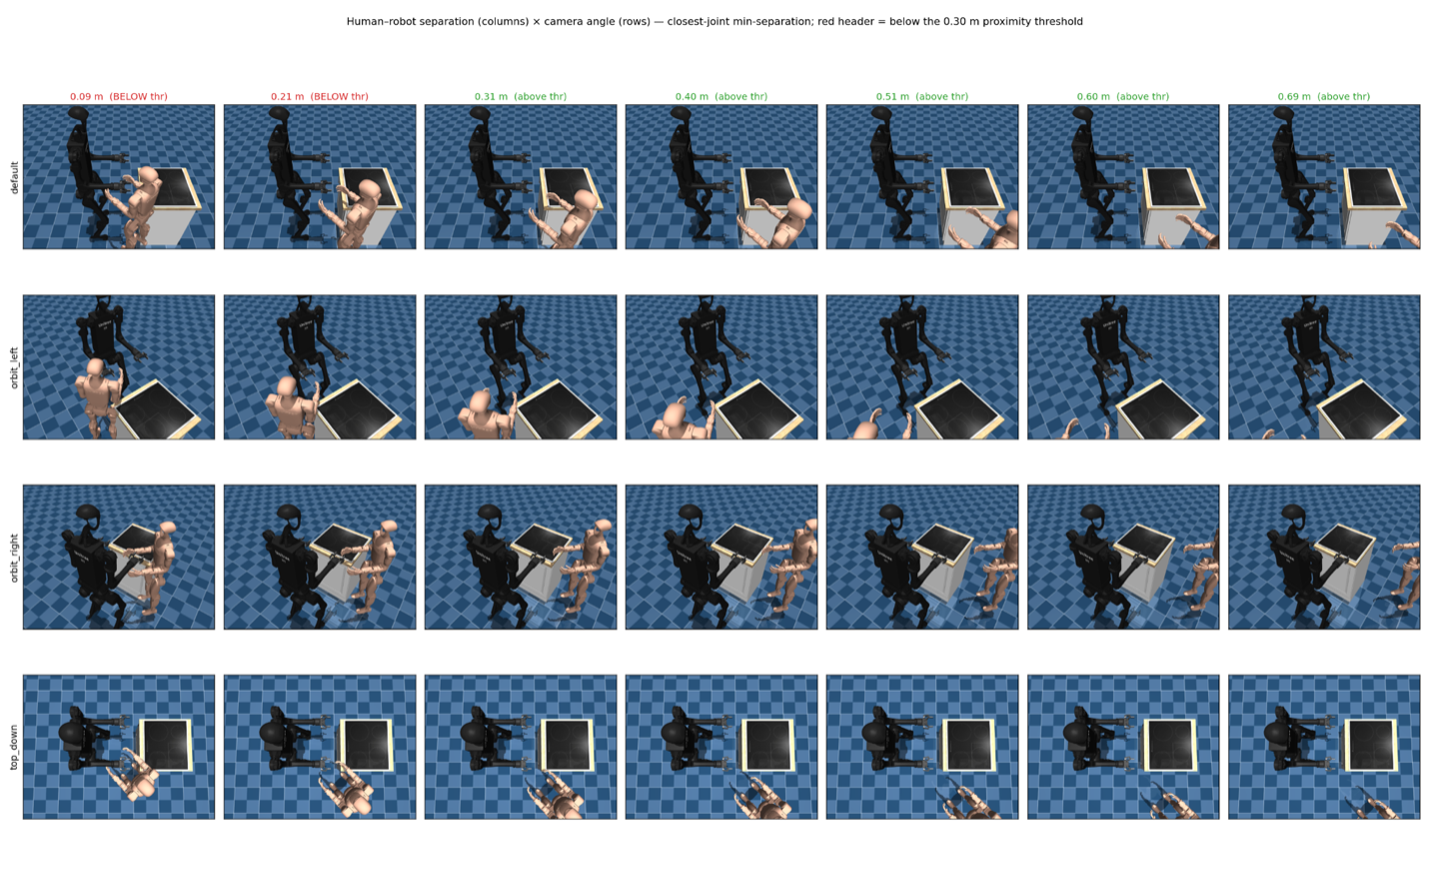
\includegraphics[width=\textwidth]{separation_render_grid.png}
\caption{Contact-geometry calibration of $\tau_{\mathrm{prox}}$. The
H1 robot (dark) and the G1 coworker (light) are rendered at seven
controlled closest-joint separations (columns) from four camera angles
(rows), with the \texttt{saucepan\_to\_hob} table between them. Red
column headers are below the $0.30$\,m proximity threshold: at $0.09$
and $0.21$\,m the body geometries visibly interpenetrate, whereas by
$0.31$\,m (green) a clear gap has opened. This confirms that $0.3$\,m
sits just above the physical contact band, so a proximity violation
fires \emph{before} contact, complementing the empirical-CDF knee of
Table~\ref{tab:prox-calib} and Figure~\ref{fig:prox-calib}.}
\label{fig:separation-scale}
\end{figure}

\paragraph{Empirical distribution.}
Because the proximity-violation rate at threshold $\tau$ is exactly the
empirical CDF $P(\min\text{-separation} < \tau)$, the threshold can be
read off the separation distribution directly. On the G1 stage-2
baseline (3 seeds, 20 episodes, 30{,}000 steps) the distribution is
bimodal, a near-contact mode at 0--0.2\,m plus a far mid-range and
patrol tail, with a knee at $\tau \approx 0.2$--$0.3$\,m
(Table~\ref{tab:prox-calib}). The knee location is consistent across
two independently trained policies, so it reflects scene contact
geometry rather than a single controller.

\begin{table}[h]
\centering
\small
\caption{Proximity-violation rate as a function of the threshold
$\tau$ (the empirical CDF of $\min$-separation on the G1 stage-2
baseline, 3 seeds $\times$ 20 episodes, 30{,}000 steps). The rate
climbs steeply once $\tau$ crosses into the benign mid-range, which is
why a $0.5$\,m or $1.0$\,m threshold would absorb a large benign
population.}
\label{tab:prox-calib}
\begin{tabular}{lccccccc}
\toprule
$\tau$ (m) & 0.20 & \textbf{0.30} & 0.40 & 0.50 & 0.60 & 0.75 & 1.00 \\
\midrule
Violation rate & 20.1\,\% & \textbf{25.3\,\%} & 29.9\,\% & 35.8\,\% & 39.5\,\% & 47.0\,\% & 62.9\,\% \\
\bottomrule
\end{tabular}
\end{table}

\begin{figure}[h]
\centering
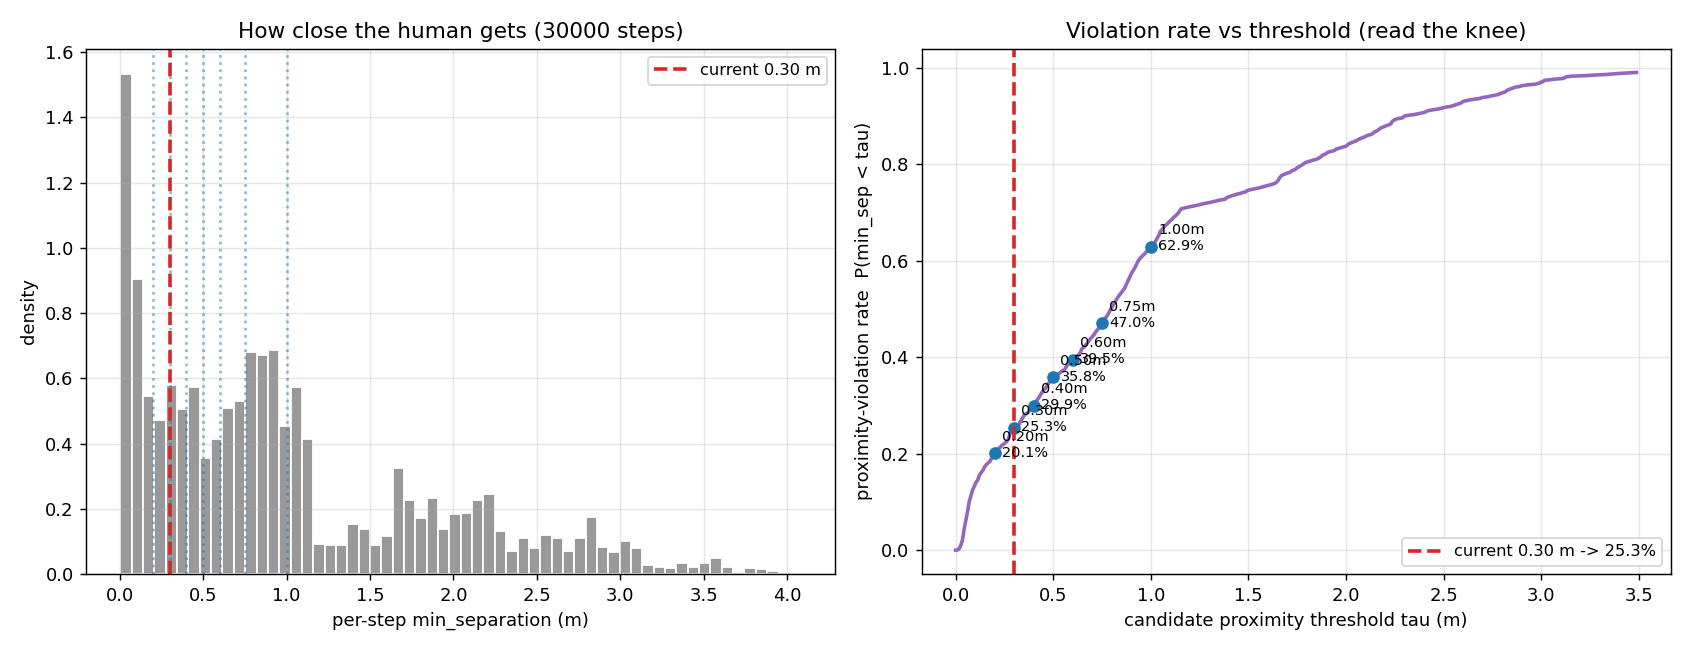
\includegraphics[width=\textwidth]{prox_calib_row5.png}
\caption{Calibrating $\tau_{\mathrm{prox}}$ on the unconstrained G1
stage-2 baseline under \texttt{coworker\_train} (30{,}000 steps).
\emph{Left:} the per-step $\min$-separation distribution is strongly
bimodal, a near-contact mode below $\sim$0.2\,m and a broad mid-/far
tail. \emph{Right:} the proximity-violation rate is the empirical CDF
$P(\min\text{-sep} < \tau)$; it rises steeply across the near-contact
mode and exhibits a knee at $\tau \approx 0.2$--$0.3$\,m (dashed line:
the chosen $\tau = 0.3$\,m).}
\label{fig:prox-calib}
\end{figure}

We fix $\tau_{\mathrm{prox}} = 0.3$\,m: it sits at the knee, $\sim$0.2\,m
above the contact band, and captures the genuine near-contact
population without absorbing the benign mid-range proximity that a
$0.5$\,m ($36\,\%$) or $1.0$\,m ($63\,\%$) threshold would. Being
purely geometric it is speed-independent, so the proximity-violation
rate is comparable across policies, tasks and disruption bands, and it
is held fixed across every experiment in this report. The
$\approx$25\,\% near-contact rate this calibration rollout induces (the
headline per-episode benchmark, Table~\ref{tab:e4.1-feature-incremental},
reports $0.296$ for the same baseline; the small difference is
per-step versus per-episode aggregation over a different episode draw)
is precisely the near-contact behaviour the constrained policy and the
runtime filters are meant to reduce.

\section{Continuous Cost Signals}
\label{sec:bench:cost}

The wrapper computes two continuous, anticipatory cost signals from
the \iso{} margins:
\begin{align}
  c^{\ssm}_t  &= \max\!\left(0,\; 1 - \frac{m^{\ssm}_t}{d_{\mathrm{buffer}}}\right),
    \label{eq:c-ssm} \\
  c^{\pfl}_t  &= \max\!\left(0,\; f^{\mathrm{ratio}}_t - 0.8\right),
    \label{eq:c-pfl} \\
  c_t         &= \min\!\left(1,\; \max(c^{\ssm}_t,\, c^{\pfl}_t)\right),
    \label{eq:c-total}
\end{align}
where $m^{\ssm}_t$ is the instantaneous \ssm{}-actual margin
(positive when safe, negative when violating), $d_{\mathrm{buffer}}
= 0.3$\,m is the anticipation buffer, and $f^{\mathrm{ratio}}_t$ is
the force-ratio from Equation~\ref{eq:iso-pfl-ratio}. The
aggregator takes the worst-case across both criteria and saturates
at $c_t = 1$.

\paragraph{Why continuous rather than binary.}
A binary indicator $c_t \in \{0,1\}$ on violation supplies only
\emph{post-hoc} gradient signal. The policy learns that crossing
the threshold is bad but receives no information about how close to
the threshold it is approaching. The continuous formulation in
Equations~\ref{eq:c-ssm}--\ref{eq:c-pfl} gives a non-zero cost
before violations occur: a \ssm{}-actual margin of $0.15$\,m carries
a cost of $\sim$0.5, and any margin beyond the $0.3$\,m buffer
carries zero. We adopt it for this gradient richness. We note in
advance, however, that the cost-signal \emph{form} turns out
\emph{not} to be the operative variable: Experiment~E3.1
(Section~\ref{sec:results:cost-signal}) shows that at a tight budget
both the continuous and the binary forms collapse, because the
binding quantity is the Lagrangian budget relative to the task's
inherent cost, not the encoding of the cost. The continuous form is
retained as the more principled design, not because it is shown to
dominate the binary one.

The choice of $d_{\mathrm{buffer}} = 0.3$\,m matches the typical
\iso{}~\ssm{} robot-stopping contribution at the H1's observed
end-effector speeds; the 0.8 threshold in Equation~\ref{eq:c-pfl}
matches the 20\,\% headroom that \iso{} Annex~A motivates for
``approaching the limit''.

\paragraph{The \pfl{} contact-detection limitation.}
\pfl{} flag computation reads MuJoCo's \texttt{data.ncon} for
human--robot contact pairs. \bigym{}'s runtime robot-attachment in
\textsc{mojo} currently produces \texttt{data.ncon = 0} for these
pairs despite geometric overlap, so $c^{\pfl}_t \equiv 0$ throughout
the project. The wrapper exposes a \texttt{use\_pfl} flag wired
through every component; the flag can be flipped on once the
contact-detection issue is resolved without architectural change.
\textbf{All quantitative compliance claims in this report are
qualified as \ssm{}/proximity-only}
(Section~\ref{sec:disc:pfl-bug}).

\section{The \coworker{} Disruption: Design and Rationale}
\label{sec:bench:coworker}

The dominant deployment pattern for human-aware manipulation is
\emph{sustained co-working}: the human is in the workspace for the
whole task, not for a one-shot intrusion. The original \bigym{}
distribution had no human at all; legacy disruption types in the
\sbigym{} ecosystem (\textsc{incidental}, \textsc{shared-goal},
\textsc{direct}, \textsc{obstruction}, \textsc{random-perturbed},
\textsc{contact}) all encoded a single intrusion event per episode
and are inadequate as a training distribution for our setting. We
introduce \textsc{Disruption.coworker} as the primary distribution
for both training and evaluation.

\subsection{Design Goals}
\label{sec:bench:coworker:design}

The \coworker{} disruption was designed against three concrete
targets:

\begin{enumerate}[topsep=2pt,itemsep=2pt]
\item \emph{Realism.} The human's behaviour should resemble what a
  real co-worker would do in a shared kitchen: enter the workspace,
  approach the task area, occasionally reach toward the task object
  or toward the robot's own arm, and occasionally step
  away for a moment. Episodes should feel like minutes of
  collaboration, not seconds of intrusion.
\item \emph{Sufficient disruption to expose unsafe behaviour.} If
  the human's reaches are rare or always far from the robot, the
  benchmark cannot discriminate safe from unsafe policies, since a
  fast-moving but careless policy would happen to be safe by luck.
  The \coworker{} band tightens the human's closest \emph{pelvis-to-pelvis}
  approach (0.60--0.95\,m) and dwell time at \textsc{near} (9--14\,s)
  so that every episode includes substantial opportunity for
  \ssm{}/proximity violations. The 0.60--0.95\,m figure is the
  body-centre separation; the reaching arm extends well inside it, so
  the closest geometry pair (hand or forearm to the robot's arm) routinely
  enters the $\tau_{\mathrm{prox}} = 0.3$\,m proximity zone, which is
  what the \texttt{proximity\_violation} flag measures. On the
  unconstrained baseline (Section~\ref{sec:results:baseline}), the
  resulting \texttt{ep\_proximity\_violation\_rate} is $0.296$ ($\approx$30\,\%),
  high enough to expose a $20+\,\%$ improvement from any of our
  safety mechanisms as statistically significant.
\item \emph{Compositional disruption modes.} A real co-worker
  exhibits at least three distinct behaviours over a session:
  staying put while reaching; walking in then staying; walking in,
  leaving briefly, and returning. The \coworker{} sampler covers all
  three but weights them unequally, drawing the most demanding mode
  (patrol) the large majority of the time so that the training
  distribution concentrates on the hardest behaviour while still
  exercising the simpler ones.
\end{enumerate}

\subsection{Three Trajectory Modes}
\label{sec:bench:coworker:traj}

A \coworker{} scenario samples one of three trajectory modes, with
the patrol mode drawn $\sim$90\,\% of the time and the two simpler
modes sharing the remaining $\sim$10\,\%:

\begin{description}[leftmargin=2em,topsep=2pt,itemsep=2pt]
\item[\textsc{stationary}] G1 spawns at \textsc{near} distance and
  stays put. Arm reaches throughout the episode.
\item[\textsc{approach-loiter-depart}] G1 spawns far, walks in to
  \textsc{near}, stays put. Arm reaches after arrival.
\item[\textsc{coworker-patrol}] G1 walks in to \textsc{near}, then
  cyclically departs to an \textsc{away} position (90°--270°
  offset, $\sim$2--3\,m), loiters, returns to a \emph{new}
  \textsc{near} position (different angle, slightly different
  distance), and repeats. Arm reaches only while at \textsc{near}.
\end{description}

The patrol mode is the most realistic operational pattern and is
therefore the dominant mode at full strength; the two simpler modes
are retained both as occasional variety in the headline distribution
and as the bulk of the earlier curriculum stages
(Section~\ref{sec:method:curriculum}), which ramp up to the
patrol-dominant mixture.

\subsection{Arm State Machine and Reach Gate}
\label{sec:bench:coworker:arm}

Independently of trajectory, the G1's reaching arm runs a four-state
cycle: \textsc{extend} (blend rest pose toward an IK target) →
\textsc{hold} (arm at target) → \textsc{retract} (blend back to
rest) → \textsc{idle} (rest pose). Default fractions of cycle
period $T$: extend 0.15, hold 0.20, retract 0.15, idle 0.50, with
$T \in [1.3, 2.2]$\,s in the train band. Each cycle samples whether
to reach for the robot's end-effector or the task object via a
\texttt{target\_mix\_p\_ee} parameter; the chosen target is
re-resolved each step so the reach tracks a moving robot or task
object. A \emph{reach gate} suppresses the IK during the
\textsc{away} phase of patrol (when the shoulder is too far from
any reachable target) and returns the rest pose, producing the
natural ``G1 walks off with arms at side'' visual. Because the arm
spends roughly half of each cycle idle and, in patrol mode, periodically
vacates the \textsc{near} zone entirely, the task remains completable
throughout: a well-behaved policy is expected to make progress during
these windows rather than halt indefinitely, which is precisely the
behaviour the success-rate axis rewards over a trivial ``freeze until
the human leaves'' strategy.

\subsection{Train and Eval Parameter Spaces}
\label{sec:bench:coworker:params}

Five \coworker{} axes are exposed as continuous
\texttt{ParameterSpace} ranges, with train and eval distributions
configured separately for the OOD generalisation experiment (E5.2):

\begin{table}[h]
\centering
\small
\caption{The \coworker{} train and eval \texttt{ParameterSpace}.
Train is moderately tight, deliberately set to produce a high
baseline violation rate (so a $20+\,\%$ safety improvement is
statistically detectable). Eval is wider, capturing the
generalisation question. The 0.60\,m closest-approach floor is the
smallest body distance that keeps the G1 mocap-pelvis collision
capsule clear of the H1 pelvis collision capsule; tighter values
generate spurious contact forces and are pathological.}
\label{tab:coworker-params}
\begin{tabular}{lcc}
\toprule
Axis & Train (\texttt{coworker\_train}) & Eval (\texttt{coworker\_eval}) \\
\midrule
Closest-approach distance     & $0.60$--$0.95$\,m  & $0.6$--$1.8$\,m  \\
Reach period $T$              & $1.3$--$2.2$\,s    & $3.0$--$9.0$\,s  \\
$P(\text{reach EE})$          & $0.45$--$0.72$     & $0.1$--$0.9$     \\
Near-loiter dwell time        & $9.0$--$14.0$\,s   & $4$--$16$\,s     \\
Walk speed                    & $1.0$--$1.4$\,m/s  & $0.6$--$2.2$\,m/s\\
\bottomrule
\end{tabular}
\end{table}

\section{The Primary Task: \texttt{saucepan\_to\_hob}}
\label{sec:bench:task}

We adopt \texttt{saucepan\_to\_hob} as the primary benchmark task.
The choice is motivated by:

\begin{enumerate}[topsep=2pt,itemsep=2pt]
\item \textbf{Long horizon for violation opportunity.}
  \texttt{saucepan\_to\_hob} is a pick-and-place task with a
  vertical clearance constraint; episodes last 30--50\,s, several
  reach cycles of the \coworker{} arm. Shorter reach-target tasks
  end before the coworker has cycled enough to expose representative
  unsafe behaviour.
\item \textbf{Workspace overlap with the coworker.} The saucepan
  pickup and the hob target are both within the H1's primary
  reach envelope, which is also where the G1 reaches when the
  reach target is the task object. Episode trajectories therefore
  pass through the same volume the coworker occupies, exposing
  real \ssm{} violations rather than incidental closeness.
\item \textbf{\bigym{}-RL competence.} Of the four candidate
  \bigym{} tasks we screened with ACT baselines, \texttt{saucepan\_to\_hob}
  combines the longest horizon with the greatest workspace overlap,
  and the unconstrained \cqnas{} agent
  (Section~\ref{sec:results:baseline}) reaches a strong
  \texttt{success\_rate} on it after the curriculum
  (Section~\ref{sec:method:curriculum}). The unconstrained baseline
  is a non-trivial reference: any safety improvement we report is
  against a competent task policy, not a policy that was failing the
  task anyway. \cqnas{} task-performance on \bigym{} is documented
  in~\cite{seo2024cqnas}.
\end{enumerate}

\section{Mock \bodyslampp{}: Calibrated Perception Noise}
\label{sec:bench:perception}

Training-time runs use ground-truth human position; deployment-time
runs use a noisy estimate. To characterise the perception
sim-to-real gap (RQ1, RQ4), we expose a configurable
\texttt{BodySLAMWrapper} with three modes:

\begin{description}[leftmargin=2em,topsep=2pt,itemsep=2pt]
\item[\texttt{off}] No human-state channel in the observation.
\item[\texttt{oracle}] Ground-truth human position injected as
  \texttt{human\_pos\_estimate} (6D: position + occluded flag +
  staleness counter + confidence).
\item[\texttt{noisy}] The full mock-\bodyslampp{} pipeline, calibrated
  against the published characteristics of~\cite{henning2023bodyslampp}.
\end{description}

The noisy pipeline applies, in order:
\begin{enumerate}[topsep=2pt,itemsep=1pt]
\item Ornstein-Uhlenbeck temporally-correlated position noise
  ($\alpha = 0.9$, $\sigma = 0.05$\,m, stationary std $\approx
  0.115$\,m), calibrated against \bodyslampp{}'s reported
  positional accuracy~\cite{henning2023bodyslampp}.
\item 3-step latency buffer ($\approx 60$\,ms at 50\,Hz control,
  matching the 15+\,FPS perception clock typical of monocular
  visual-inertial pose estimation).
\item Stochastic tracking dropout ($p = 0.02$/step) with staleness
  counter; OU state continues to update during dropout, so
  recovery is smooth rather than discontinuous.
\item Optional ray-cast occlusion from the H1's head camera
  (opt-in).
\end{enumerate}

\paragraph{Demo-replay path.}
Cached \bigym{} demonstrations~\cite{chernyadev2024bigym} were
recorded \emph{without} a coworker; their
\texttt{human\_pos\_estimate} would be missing if read live. The
wrapper supports a \texttt{mode=demo\_replay} path that synthesises
\texttt{human\_pos\_estimate} from an
\texttt{AMASSDemoPositionProvider}~\cite{mahmood2019amass} playing
back a real motion clip, so a behaviour-cloning pretraining phase
sees realistic human state at training time without a train→eval
distribution shift on the channel.

\section{Demonstrations and the Demo-Conversion Pipeline}
\label{sec:bench:demos}

\cqnas{}~\cite{seo2024cqnas} is a demo-driven RL agent: the
algorithm assumes $\text{num\_demos} > 0$ at construction.
Running with $\text{num\_demos} = 0$ on a long-horizon manipulation
task such as \texttt{saucepan\_to\_hob} fails for two reasons.
First, the sparse task reward is never discovered, so the only
training gradient is the violation penalty, and the policy learns
the cheap thing (workspace evacuation). Second, \cqnas{}'s replay
buffer stripes episodes by \texttt{eps\_idx mod num\_workers}; the
first cold-start batch can request an episode from a worker that
has no episodes yet, raising an \texttt{IndexError}.

The demo path uses the raw, non-safety-wrapped \bigym{}
environment to match \texttt{DemoStore}'s class-name lookup,
fetches 10--36 cached demonstrations, and converts each to a list of
\texttt{ExtendedTimeStep} carrying the synthesised
\texttt{human\_pos\_estimate} channel and a placeholder $c_t = 0.0$
(the cached demos contain no live human; safe-side is the
defensible value, and the curriculum stages of
Section~\ref{sec:method:curriculum} make this not a
distribution-shift issue in practice).

Five action-normalisation pitfalls fixed during integration are
documented in Section~\ref{sec:impl:integration}; the most consequential is
that \cqnas{}'s normalisation must use \emph{demo-derived} action
statistics for the live and demo distributions to share a binning.
% =============================================================================
% PART III: A HYBRID SAFETY ARCHITECTURE (the solution)
% =============================================================================

% =============================================================================
\chapter{The Hybrid Safety Architecture and Its Implementation}
\label{ch:method}
% =============================================================================

\section{Overview: From Problem to Solution}
\label{sec:method:overview}

Chapter~\ref{ch:benchmark-env} introduced \sbigym{} as the
benchmark and Section~\ref{sec:bench:why} listed six concrete
properties the benchmark is designed to test. The unconstrained
\cqnas{}~\cite{seo2024cqnas} baseline that ships with \bigym{}
fails almost all six: it has no representation of human position,
no \ssm{} margin, no constraint that would distinguish a
task-completing trajectory from one that endangers the coworker,
and Section~\ref{sec:results:baseline} will show that it registers
proximity violations on $\approx$30\,\% of steps (mean separation only
$0.13$\,m, with the worst approaches within a few millimetres), far
above what any plausible co-working deployment would accept.

This chapter presents \textbf{our solution to that gap}: a hybrid
safety architecture that turns the unconstrained
imitation-or-RL policy into an \iso{}-compliant collaborator. The
architecture has two mechanisms with deliberately different roles:

\begin{enumerate}[topsep=2pt,itemsep=2pt]
\item A \textbf{training-time mechanism} that \emph{internalises}
  safety into the policy via a value-based Lagrangian formulation
  of the continuous cost signal. At deployment, the policy is
  used as-is; the safety knowledge is baked into the learned
  $Q$-functions (Section~\ref{sec:method:lagrangian}).
\item A \textbf{deployment-time mechanism}: a runtime \emph{filter
  slot} that intercepts the policy's proposed actions. The slot is
  mechanism-agnostic, and we specify and evaluate the complete
  reactive taxonomy through it: an offline-trained, frozen safety
  value function (SVF) used as a veto, the original design
  (Section~\ref{sec:method:filter}), plus two closed-form
  alternatives, a graded \iso{} speed-scaling rule and a model-based
  geometric dodge (Section~\ref{sec:method:filter:closedform}).
\end{enumerate}

Both mechanisms share a network shape and an observation interface,
which keeps the two safety critics directly comparable and leaves SVF
reuse available as an option, though the constrained policy's cost
critic is in fact cold-started
(Section~\ref{sec:method:lagrangian:warmstart}); they differ in
training objective and operational role. The full pipeline at
deployment is sketched in Figure~\ref{fig:hybrid-overview}.

\begin{figure}[h]
\centering
\resizebox{\textwidth}{!}{%
\begin{tikzpicture}[
  >=Latex, node distance=10mm and 11mm,
  box/.style={draw, rounded corners, align=center, inner sep=4pt,
              minimum height=11mm, font=\small},
  env/.style={box, fill=black!5},
  pol/.style={box, fill=blue!8, draw=blue!55, minimum width=42mm},
  filt/.style={box, fill=orange!12, draw=orange!70, minimum width=34mm},
  trn/.style={box, dashed, fill=black!3, draw=black!45, align=center,
              font=\footnotesize, text=black!75, minimum height=10mm},
  flow/.style={->, thick},
  tflow/.style={->, thick, dashed, black!55},
]
% --- deployment row ---
\node[env] (env) {Environment\\[-1pt]{\footnotesize \textsc{BiGym} $+$ G1 coworker}};
\node[box, right=of env] (obs) {Observation $s_t$\\[-1pt]{\footnotesize proprio.\ $+\ \hat p_{\mathrm{human}}$}};
\node[pol, right=of obs] (pol) {Policy $\pi$\\[2pt]$a^{\mathrm{nom}}=\mathrm{argmax}_{a}[\,Q_r-\lambda Q_c\,]$};
\node[filt, right=of pol] (filt) {Runtime filter\\[2pt]$Q_{\mathrm{safe}}(s,a^{\mathrm{nom}})\ge R$\,?};
\node[box, right=of filt] (exec) {Execute $a_t$};

\draw[flow] (env) -- (obs);
\draw[flow] (obs) -- (pol);
\draw[flow] (pol) -- (filt);
\draw[flow] (filt) -- node[above,font=\footnotesize]{pass}
                      node[below,font=\footnotesize]{$a_t{=}a^{\mathrm{nom}}$} (exec);

% --- veto branch ---
\node[box, fill=orange!5, draw=orange!55, font=\footnotesize,
      minimum height=8mm, below=9mm of filt] (fb) {fallback $a^{\mathrm{fb}}$};
\draw[flow] (filt.south) -- node[right,font=\footnotesize]{veto} (fb.north);
\draw[flow] (fb.east) -| (exec.south);

% --- feedback loop ---
\draw[flow] (exec.north) -- ++(0,7mm) -| (env.north);

% --- training band ---
\node[trn, below=15mm of pol] (lag)
  {trained \emph{online}: value-based\\ Lagrangian on cost $c_t$
   $\;\Rightarrow\; Q_r,Q_c$};
\node[trn, below=15mm of fb] (cql)
  {trained \emph{offline} (CQL),\\ frozen at deployment
   $\;\Rightarrow\; Q_{\mathrm{safe}}$};
\draw[tflow] (lag) -- (pol);
\draw[tflow] (cql.north) -- (filt.west);
\end{tikzpicture}%
}
\caption{The hybrid safety architecture at deployment. At each step
the Lagrangian-trained policy proposes the nominal action
$a^{\mathrm{nom}} = \mathrm{argmax}_a\,[Q_r(s,a) - \lambda Q_c(s,a)]$;
a runtime filter passes it through when its safety check holds and
otherwise substitutes a fallback action. The two mechanisms have
deliberately different jobs: the constrained policy internalises
safety \emph{proactively} during training, while the filter is a
\emph{reactive} runtime mechanism. Chapter~\ref{ch:eval} shows that
how these compose is not obvious in advance: a learned veto calibrated
to the unconstrained baseline is counterproductive on the avoiding
policy, whereas a complementary-axis speed-scaling filter composes
additively. The resulting division of labour, proximity from the
policy and velocity from the filter, is quantified in
Table~\ref{tab:e4.1-feature-incremental} and
Figure~\ref{fig:joint-coverage}.}
\label{fig:hybrid-overview}
\end{figure}

\section{The Offline Safety Value Function (Phase~2)}
\label{sec:method:filter}

\subsection{Dataset and Labelling}
\label{sec:method:filter:data}

The SVF is trained offline on a dataset of transitions collected by
rolling out \cqnas{} policy snapshots from the base-policy curriculum
(Section~\ref{sec:method:curriculum}) in the \coworker{} distribution
under the \texttt{noisy} observation mode. Earlier iterations of the
critic mixed random-policy and demonstration transitions; the current
critic is collected from policy snapshots alone. The reasoning is that
the regions a deployed policy actually visits are precisely the regions
the filter must judge accurately, and snapshot rollouts sample exactly
that on-policy distribution, including the imitation-learning artefacts
a competent-but-imperfect policy exhibits under sustained co-working
disruption. The filter is \emph{noisy-native}: it is trained and
evaluated on \texttt{noisy} human-state estimates, and on
ground-truth (\texttt{oracle}) input its $Q$-estimates collapse and it
intervenes almost everywhere, so all filtered evaluations are reported
on \texttt{noisy} (Section~\ref{sec:setup:perception-mode}). The exact
transition count for the current critic is 37{,}883, of which
$16.8\,\%$ are labelled unsafe ($r^{\mathrm{safe}} = 0$) at the
$\tau = 0.3$\,m proximity threshold; the full figures are in the
Phase~2 results write-up.

Each transition is labelled with the binary safety reward
\begin{equation}
  r^{\mathrm{safe}} \;=\; 1 - \mathbb{1}[\texttt{proximity\_violation}],
  \label{eq:r-safe}
\end{equation}
using the geometric proximity-violation flavour of
Section~\ref{sec:bench:metrics:flavours} at the calibrated threshold
$\tau_{\mathrm{prox}} = 0.3$\,m (the calibration is derived in
Section~\ref{sec:bench:proximity-threshold}). We label on
\texttt{proximity\_violation} rather than \texttt{ssm\_violation\_actual}
for two reasons. First, the conservative-ISO \ssm{} flag is saturated:
it fires on $\sim$93\,\% of random rollouts and remains high even for
competent policies because it assumes the worst-case human velocity, so
it carries almost no gradient for a value function to learn. Second, and
by design, labelling on geometry keeps a clean separation of concerns
between the two safety mechanisms. The runtime filter is made
responsible for the \emph{geometric} danger of being too close, while
the velocity-dependent \ssm{} response is left to the cost signal and
the constrained policy (Section~\ref{sec:method:lagrangian}). Coupling
the filter's training target to instantaneous velocity would make its
label depend on the very action it is meant to veto, conflating ``how
dangerous is this configuration'' with ``how fast is the robot moving'',
the latter being a decision the policy, not the filter, should own.

Because the violating class is the minority, a
\texttt{WeightedRandomSampler} over-samples it to a $1{:}1$ ratio of
safe to violating transitions per batch, so the critic is not
dominated by the safe majority.

\subsection{Architecture and Training}
\label{sec:method:filter:arch}

The safety critic is a 3-layer MLP with hidden sizes
$[256, 256, 256]$ and ReLU activations. The input is the
concatenation of robot proprioception, the mock-\bodyslampp{} 6D
human-position estimate, and the proposed action. The output is
bounded to $[0, q_{\max}]$ with $q_{\max} = 1/(1-\gamma)$ via a
scaled sigmoid, which \emph{mathematically} prevents Bellman
overestimation: $Q$ cannot exceed the maximum possible discounted
return of a safe trajectory.

Training combines a Bellman residual with the
\textsc{CQL}~\cite{kumar2020cql} regulariser:
\begin{equation}
  \mathcal{L} \;=\; \mathcal{L}_{\mathrm{Bellman}}
  \;+\; \alpha_{\mathrm{CQL}} \cdot
  \left(\mathbb{E}_{a \sim \mathrm{uniform}}\!\left[Q(s,a)\right]
       - \mathbb{E}_{a \sim \mathcal{D}}\!\left[Q(s,a)\right]\right),
  \label{eq:cql-loss}
\end{equation}
with $\alpha_{\mathrm{CQL}} = 5.0$ as the headline value, Polyak
target update $\tau = 0.005$. Full training hyperparameters in
Appendix~\ref{app:hparams:svf}.

\subsection{No-Pixel Critic: Justification}
\label{sec:method:filter:nopixels}

The filter does not consume RGB. Three reasons against the obvious
alternative (an RGB-consuming critic like the actor):

\begin{enumerate}[topsep=2pt,itemsep=1pt]
\item \emph{Compute.} 50\,Hz control at 76 DOF affords $\sim$20\,ms
  per step; a CNN-encoder forward pass is a substantial fraction
  of that budget. A pure-MLP critic is $\sim$0.3\,ms per forward.
\item \emph{Robustness.} An RGB critic depends on lighting and
  texture domain shift between train and deployment. A
  human-position-vector critic depends only on the upstream pose
  estimator's calibration~\cite{henning2023bodyslampp}.
\item \emph{Compositionality.} The filter is portable across
  policies. A no-pixel filter wraps any policy whose observation
  is a subset of $\{$proprio, $\hat{p}^{\mathrm{human}}$, proposed
  action$\}$.
\end{enumerate}

\subsection{Runtime Wrapper}
\label{sec:method:filter:runtime}

At deployment, the \texttt{SafetyFilterWrapper} intercepts the
proposed action and compares the safety value against a threshold
$R$:
\begin{equation}
  a^{\mathrm{exec}}_t \;=\;
  \begin{cases}
    a^{\mathrm{nom}}_t   & \text{if } Q_{\mathrm{safe}}(s_t, a^{\mathrm{nom}}_t) \ge R, \\
    a^{\mathrm{fb}}_t    & \text{otherwise.}
  \end{cases}
  \label{eq:filter-rule}
\end{equation}
$R$ is calibrated by sweep over a held-out validation set
(Experiment~E2.3, Section~\ref{sec:results:filter-pareto}); the
headline operating point for the G1 critic on the \coworker{}
distribution is $R = 2.25$. (An earlier operating point of $R = 4.0$
was calibrated against the superseded SMPL-H critic and did not
transfer to the G1 stand-in, which has a different separation
distribution; the G1 value is the one pinned in the released
snapshots.) The intended role of the filter at this operating point
is an \iso{}~\ssm{} \emph{velocity backstop} rather than a proximity
reducer: it intervenes on the small fraction of steps where the
robot's own motion would breach the velocity-dependent separation
requirement, and is not expected to cut geometric proximity on its
own, since much of the residual proximity is the human walking up to
an otherwise stationary robot. Section~\ref{sec:results:filter-pareto}
quantifies this division of labour.

The Phase~2 fallback is zero-velocity braking on the floating base
and on every joint velocity actuator. This can produce abrupt
motion mid-trajectory; proportional damping is the natural upgrade
and is deferred to future work (Section~\ref{sec:fw:fallback}).

\section{Closed-Form Runtime Filters: Speed-Scaling and Geometric Dodge}
\label{sec:method:filter:closedform}

The filter slot of Figure~\ref{fig:hybrid-overview} is
mechanism-agnostic: anything that maps the state and the proposed
action $(s_t, a^{\mathrm{nom}}_t)$ to an executed action can occupy
it. The learned SVF veto above is its learned instantiation. Two
\emph{closed-form} mechanisms, specified here and evaluated alongside
the veto in Chapter~\ref{ch:eval}, complete the reactive taxonomy:
stop (veto), slow (speed-scaling), and move away (dodge). Both
consume the same $\hat{p}^{\mathrm{human}}$ estimate as the SVF and
contain no learned component.

\subsection{Graded \iso{} Speed-Scaling}
\label{sec:method:filter:speedscale}

\iso{}~\ssm{}'s intent is graded: the robot should \emph{slow} as
separation shrinks, not merely stop at a threshold. The speed-scaling
filter implements this directly. At each step a scale factor is
computed from the closest-pair human--robot separation
$\mathrm{sep}_t$,
\begin{equation}
  \sigma_t \;=\; \mathrm{clip}\!\left(
    \frac{\mathrm{sep}_t - d_{\mathrm{stop}}}
         {d_{\mathrm{slow}} - d_{\mathrm{stop}}},\; 0,\; 1\right),
  \qquad
  a^{\mathrm{exec}}_t \;=\; q_t + \sigma_t \,
    \bigl(a^{\mathrm{nom}}_t - q_t\bigr),
  \label{eq:speed-scale}
\end{equation}
where $q_t$ is the current joint position for the absolute-mode arm
dimensions (so the per-step \emph{motion} from the current pose is
scaled) and zero for the delta-mode floating base (so the commanded
increment is scaled directly). Above $d_{\mathrm{slow}}$ the filter
is the identity ($\sigma_t = 1$, byte-for-byte pass-through); at or
below $d_{\mathrm{stop}} = 0.15$\,m the robot holds position
($\sigma_t = 0$); in between, speed falls linearly with separation.
The slow radius $d_{\mathrm{slow}}$ is the single operating-point
knob, swept over $[0.25, 0.60]$\,m with the headline at $0.40$\,m;
an intervention is any step with $\sigma_t < 1$. Unlike the veto,
this filter preserves the \emph{direction} of the policy's motion
and modulates only its magnitude, which is why it can maintain the
graded velocity margin the standard prescribes where a binary
stop-or-go veto cannot
(Section~\ref{sec:results:headline-feature-table}).

\subsection{Model-Based Geometric Dodge}
\label{sec:method:filter:dodge}

The second closed-form mechanism is a geometric
control-barrier-style fallback: when the closest-pair separation
falls below a target $d_{\mathrm{target}}$, the filter adds a
correction step directed \emph{away} from the human, proportional to
the violation depth $(d_{\mathrm{target}} - \mathrm{sep}_t)$ and
capped per step. Two variants differ in which part of the robot
dodges: the \emph{base-dodge} pushes the floating base along the
escape direction and leaves the arm untouched, while the
\emph{end-effector retract} (``flinch'') keeps the base planted and
retracts the end-effector along the escape direction via a
damped-Jacobian step. $d_{\mathrm{target}}$ is swept over
$[0.30, 0.55]$\,m. These variants exist to test whether a
\emph{dodging} reactive response escapes the limits of the
\emph{stopping} one; Section~\ref{sec:results:reactive-taxonomy}
shows it does not (it trades the veto's freeze for a flee). The
headline composition deploys the policy with the speed-scaling
filter; the veto and the dodges are reported as taxonomy points
(Table~\ref{tab:filter-taxonomy}), with operating-point values for
all three mechanisms in Appendix~\ref{app:hparams:hybrid}.


\section{Value-Based Lagrangian Constrained RL (Phase~3)}
\label{sec:method:lagrangian}

\subsection{Why Value-Based}
\label{sec:method:lagrangian:why}

\cqnas{}~\cite{seo2024cqnas} is \emph{critic-only}: the policy is
implicit, $\pi(s) = \mathrm{argmax}_{a \in
\mathcal{A}_{\mathrm{bin}}} Q(s, a)$, over a coarse-to-fine
discretisation of the joint action space. The classical
actor-critic Lagrangian formulation~\cite{ray2019safetygym,
stooke2020pid} updates a policy network $\pi_\theta$ to maximise
$\mathbb{E}[Q_r(s,a)] - \lambda \mathbb{E}[Q_c(s,a)]$, which
presumes that $\pi_\theta$ exists as a separately-trained network.
There is no $\pi_\theta$ in \cqnas{}. The Lagrangian must be
re-expressed in value-based form.

Three options were considered, in increasing principledness; the
choice is itself an empirical comparison
(Experiment~E3.1).

\subsection{Option A-value: Shaped-Reward Single Critic}
\label{sec:method:lagrangian:A}

The simplest re-formulation folds the cost into a modified reward
and trains a single critic:
\begin{equation}
  r^{\mathrm{mod}}_t \;=\; r^{\mathrm{task,shaped}}_t \;-\; \lambda \cdot c_t,
  \qquad
  Q(s,a) \approx \mathbb{E}\!\left[\sum_t \gamma^t r^{\mathrm{mod}}_t\right],
  \label{eq:option-A}
\end{equation}
with action selection $a^* = \mathrm{argmax}_a Q(s,a)$. This is
attractive for its simplicity but has a known pathology: the
regression target $r^{\mathrm{mod}}_t$ is \emph{non-stationary} in
$\lambda$, which is itself non-stationary in the rolling cost. The
critic chases a moving target and oscillates. Used here as a
prototype baseline only; Experiment~E3.1 quantifies the gap to
dual-critic options.

\subsection{Option B-value-mean: Dual Q-Functions on Mean Cost (Headline)}
\label{sec:method:lagrangian:Bmean}

Decouple the reward and cost critics:
\begin{align}
  Q_r(s,a) &\approx \mathbb{E}\!\left[\sum_t \gamma^t r^{\mathrm{task,shaped}}_t\right], \\
  Q_c(s,a) &\approx \mathbb{E}\!\left[\sum_t \gamma^t c_t\right],
\end{align}
each regressing toward its own \emph{stationary} target. The action
selection combines them at decision time:
\begin{equation}
  a^* \;=\; \mathop{\mathrm{argmax}}_{a \in \mathcal{A}_{\mathrm{bin}}}
  \Big[\,Q_r(s,a) \;-\; \lambda \cdot Q_c(s,a)\,\Big].
  \label{eq:Bmean-select}
\end{equation}
$\lambda$ now enters only at selection, not at regression. The
cost critic shares its network shape with the Phase~2 SVF, so SVF
reuse is available, though here the cost critic is cold-started
(Section~\ref{sec:method:lagrangian:warmstart}). This is the
\textbf{headline architecture} for this work.

\begin{figure}[h]
\centering
\resizebox{\textwidth}{!}{%
\begin{tikzpicture}[
  >=Latex,
  cu/.style={draw, rounded corners, align=center, inner sep=3pt,
             font=\footnotesize, minimum height=8mm, minimum width=15mm},
  sel/.style={draw, rounded corners, align=center, inner sep=3pt,
              font=\footnotesize, fill=black!4, minimum height=9mm},
  io/.style={font=\footnotesize},
  title/.style={font=\small\bfseries, align=center},
  ar/.style={->, semithick},
]
% ===================== Panel A =====================
\node[io] (Ain) at (0,0) {$(s,a)$};
\node[cu, above=7mm of Ain] (Aq) {single critic $Q$\\ on $r'=r-\lambda c$};
\node[sel, above=7mm of Aq] (Asel) {$\mathrm{argmax}_{a}\,Q$};
\node[io, above=6mm of Asel] (Aout) {$a^{\ast}$};
\node[title, above=4mm of Aout] (At) {Option~A\\[-1pt]{\scriptsize (prototype)}};
\draw[ar] (Ain)--(Aq); \draw[ar] (Aq)--(Asel); \draw[ar] (Asel)--(Aout);

% ===================== Panel B-mean (headline) =====================
\node[io] (Bin) at (5.4,0) {$(s,a)$};
\node[cu, above left=8mm and 1mm of Bin]  (Bqr) {$Q_r$};
\node[cu, above right=8mm and 1mm of Bin] (Bqc) {$Q_c$};
\node[sel, above=20mm of Bin] (Bsel) {$\mathrm{argmax}_{a}$\\$[\,Q_r-\lambda Q_c\,]$};
\node[io, above=6mm of Bsel] (Bout) {$a^{\ast}$};
\node[title, above=4mm of Bout] (Bt) {Option~B-value-mean\\[-1pt]{\scriptsize (headline)}};
\draw[ar] (Bin)--(Bqr); \draw[ar] (Bin)--(Bqc);
\draw[ar] (Bqr)--(Bsel); \draw[ar] (Bqc)--(Bsel); \draw[ar] (Bsel)--(Bout);

% ===================== Panel B-CVaR =====================
\node[io] (Cin) at (11.0,0) {$(s,a)$};
\node[cu, above left=8mm and 1mm of Cin]  (Cqr) {$Q_r$};
\node[cu, above right=8mm and 1mm of Cin] (Cqc) {dist.\ $Z_c$};
\node[sel, above=20mm of Cin] (Csel) {$\mathrm{argmax}_{a}$\\$[\,Q_r-\lambda\,\cvar_{\alpha}(Z_c)\,]$};
\node[io, above=6mm of Csel] (Cout) {$a^{\ast}$};
\node[title, above=4mm of Cout] (Ct) {Option~B-value-CVaR\\[-1pt]{\scriptsize (future work)}};
\draw[ar] (Cin)--(Cqr); \draw[ar] (Cin)--(Cqc);
\draw[ar] (Cqr)--(Csel); \draw[ar] (Cqc)--(Csel); \draw[ar] (Csel)--(Cout);

% highlight the headline panel
\begin{scope}[on background layer]
\node[rounded corners, fill=blue!7, fit=(Bin)(Bqr)(Bqc)(Bsel)(Bout)(Bt),
      inner sep=4pt] {};
\end{scope}
\end{tikzpicture}%
}
\caption{The three value-based formulations of the Lagrangian on top
of the critic-only \cqnas{} backbone. Option~A folds the cost into a
single shaped-reward critic and is unstable because its regression
target moves with $\lambda$; Option~B-value-mean adds a separate cost
critic $Q_c$ so that $\lambda$ enters only at action selection,
$\mathrm{argmax}_a[Q_r - \lambda Q_c]$; Option~B-value-CVaR replaces
the mean cost critic with a distributional one. B-value-mean (centre)
is the headline architecture, the simplest formulation with a
stationary regression target for each critic. Option~A is a prototype
baseline and B-CVaR is future work (Section~\ref{sec:fw:cvar}).}
\label{fig:lagrangian-architectures}
\end{figure}

\subsection{Option B-value-CVaR: Distributional Cost Critic (future work)}
\label{sec:method:lagrangian:Bcvar}

A natural extension replaces the mean-cost critic with a
distributional one: $Q_c$ is replaced by either a Gaussian
parametrisation $(\mu_c, \sigma_c)$~\cite{yang2021wcsac} or a
quantile head $\{\theta_k\}_{k=1}^K$~\cite{dabney2018qrdqn}, with
action selection
\begin{equation}
  a^* \;=\; \mathop{\mathrm{argmax}}_{a \in \mathcal{A}_{\mathrm{bin}}}
  \Big[\,Q_r(s,a) \;-\; \lambda \cdot \cvar_{\alpha}(Z_c \mid s, a)\,\Big],
\end{equation}
with $\alpha \in \{0.95, 0.99\}$. This aligns the training-time
objective with the evaluation metric (\cvar{} on the headline tail
plots) and answers the standard critique that mean-cost Lagrangian
methods bound only $\mathbb{E}[Z_c]$, not the tail. \cqnas{}'s
critic is already C51-distributional~\cite{bellemare2017c51};
adding a second distributional cost head is a small extension.
However, calibrating the distinct rolling target (rolling-\cvar{}
of episode cost vs.\ rolling-mean) and verifying that the C51
support assumption from Section~\ref{sec:method:lagrangian:support}
holds for the cost distribution adds non-trivial engineering.
\textbf{We adopt B-value-mean as the headline and report
explicit-\cvar{} training as future work
(Section~\ref{sec:fw:cvar})}; in
Section~\ref{sec:results:tail} we evaluate the mean-policy's
\emph{achieved} \cvar{} as a diagnostic.

\subsection{The C51 Value-Support Invariant}
\label{sec:method:lagrangian:support}

\cqnas{} uses a C51 distributional reward critic with fixed value
support $[v_{\min}, v_{\max}]$~\cite{bellemare2017c51}. The Bellman
target $T_z = r + \gamma \cdot \mathrm{support}$ is clamped to this
support at each update. Adding a dense shaped reward term such as
Equation~\ref{eq:r-workspace} introduces a discounted return whose
value can fall outside the support; once the target is clamped, the
critic loses the ability to distinguish values in the saturating
region, and the gradient that should pull the end-effector back
toward the task is clipped away.

\begin{proposition}[Support-bounding invariant]
\label{lem:support-bound}
Let a C51 distributional critic have value support
$[v_{\min}, v_{\max}]$, discount $\gamma$, and an additive shaped
reward $r^{\mathrm{shaped}}_t \in [-\beta \cdot c_{\mathrm{ws}}, 0]$
with $\beta, c_{\mathrm{ws}} > 0$. The shaped-reward contribution
to the discounted return is bounded by
$\beta \cdot c_{\mathrm{ws}} / (1 - \gamma)$ in magnitude. The
Bellman target clamp is informative (i.e., the support is not
saturated) only if
\begin{equation}
  \beta \cdot c_{\mathrm{ws}} \,/\, (1-\gamma) \;\le\; |v_{\min}|.
  \label{eq:support-invariant}
\end{equation}
\end{proposition}

\begin{proof}
The geometric-series sum of the per-step shaping under the worst
case gives $\sum_{t=0}^\infty \gamma^t \beta c_{\mathrm{ws}} =
\beta c_{\mathrm{ws}} / (1-\gamma)$, and the C51 target clamp
clips below $v_{\min}$. \qed
\end{proof}

\paragraph{Consequence.}
The original workspace shaping ($\beta = 0.2$, no cap on per-step
excess distance) gave a worst-case discounted return of
$-0.2 / 0.01 = -20$ against the default \cqnas{} support of
$[-2, +2]$, saturating every state outside $\sim$0.5\,m of the
task. Training diverged: \texttt{ep\_reward} fell monotonically
from $-78$ to $-775$ over 50k frames as the policy parked further
from the workspace and the support flattened. The fix is
two-sided: cap the per-step penalty ($c_{\mathrm{ws}} = 1.0$\,m),
reduce $\beta$ to 0.05, and widen the support to
$[v_{\min}, v_{\max}] = [-6, +2]$. With these settings the
invariant holds ($0.05 \cdot 1.0 / 0.01 = 5 \le 6$) and training
proceeds normally; the next-attempt \texttt{ep\_reward} reaches
$\sim +1.8$ on stage~1 of the curriculum
(Section~\ref{sec:method:curriculum}).

\textbf{This is the report's strongest engineering lesson.} It
generalises to any distributional critic + dense shaping setting
and applies as a checking principle independent of \sbigym{}.

\subsection{Per-Env-Step Cost Backup}
\label{sec:method:lagrangian:per-step}

\cqnas{} executes \emph{action sequences} of length $K$ between
policy queries (coarse-to-fine refinement). A natural but subtly
wrong design is to backup the cost critic on the chunk-averaged
cost $\bar{c} = (1/K) \sum_{k} c_{t+k}$. The policy can satisfy a
mean-over-chunk budget while spiking violations \emph{inside} a
chunk. The cost critic must be backed up on \emph{every} env-step's
$c_t$. Our training pipeline preserves $c_t$ through the replay
buffer at per-env-step granularity
(Section~\ref{sec:impl:integration}).

\subsection{PID Lagrange Multiplier Update}
\label{sec:method:lagrangian:pid}

The Lagrange multiplier is updated by a PID
controller~\cite{stooke2020pid} on the running constraint violation.
Let $m_t$ be the rolling per-episode cost mean and $d$ the cost
budget; the update is
\begin{align}
  e_t &= m_t - d, \\
  \lambda_{t+1} &= \mathrm{clip}\!\left(\lambda_t + K_I \cdot e_t
    + K_P \cdot e_t + K_D \cdot (e_t - e_{t-1}),
    \; 0,\; \lambda_{\max}\right).
  \label{eq:pid-lambda}
\end{align}
PID is preferred over gradient ascent
($\lambda \leftarrow \lambda + \eta \cdot e_t$) because the
integral term provides faster convergence to the constraint
boundary while the derivative term damps
oscillation~\cite{stooke2020pid}. We use $K_I = 10^{-3}$,
$K_P = 10^{-2}$, $K_D = 0$, and $\lambda_{\max} = 100$. The clamp
prevents the policy from collapsing into a fully-frozen
``safe-and-useless'' attractor when the cost budget is briefly
violated.

\paragraph{PID auto-tuning is seed-unstable at the feasibility
boundary; a fixed multiplier is the fix.}
A finding that emerged only at deployment-faithful evaluation
(Section~\ref{sec:results:headline-feature-table}) is that the PID
controller is \emph{seed-unstable} at the only cost budget that is
both feasible and non-trivial for this task. The per-step cost
$c_t \in [0,1]$ and the task itself incurs an inherent mean cost of
$\approx$0.25--0.30 (the unconstrained baseline already sits at
proximity $0.296$), so any budget $d \le 0.2$ is below the task's
inherent cost and the only feasible policy is to abandon the task,
while $d = 0.5$ leaves the constraint slack ($\lambda \to 0$,
recovering the unconstrained policy). The single viable budget,
$d = 0.3$, sits \emph{at} the task's inherent cost, so the dual
variable is decided by each seed's stochastic cost trajectory rather
than by design: across three seeds at $d = 0.3$, $\lambda$ converged
to $0.000$, $0.267$, and $3.855$, producing respectively an
unconstrained policy, a graceful avoidance basin, and a windup
collapse to zero task success
(Figure~\ref{fig:lambda-regimes}). The graceful regime therefore
reproduced in only one of three seeds.

The fix is to remove the auto-tuning: \emph{freezing} $\lambda$ at a
constant (zero PID gains, with $Q_c$ still trained and used in
dual-action selection) makes all three seeds behave consistently and
turns $\lambda$ into a clean proximity--success Pareto knob. We sweep
it and adopt $\lambda = 0.1$ as the headline operating point: it
reaches the graceful point (proximity $0.228$, success $0.76$, robust
across three seeds), whereas $\lambda = 0.27$ over-constrains (success
$\approx$0.60) and $\lambda = 0$ recovers the baseline
(Section~\ref{sec:results:headline-feature-table},
Figure~\ref{fig:fixlam}). The methodological lesson generalises: for a
constrained policy whose only feasible budget coincides with the
task's inherent cost, the dual variable carries too little signal to
be auto-tuned stably, and a fixed or scheduled multiplier is
preferable to PID control. We retain the PID path in the codebase and
report it as the negative result that motivates the fixed-$\lambda$
headline.

\subsection{Filter During Training (optional)}
\label{sec:method:lagrangian:filter-train}

The runtime safety filter of Section~\ref{sec:method:filter} can
also be applied at training time, interposed between the proposed
action and the environment, vetoing catastrophically unsafe
proposals with the fallback~\cite{cbfrl2024,shield2025}. We report
results without the training-time filter as the default; the
filter-during-training ablation is deferred to future work
(Section~\ref{sec:fw:filter-during-training}).

\subsection{Cost-Critic Initialisation and Policy Warm-Start}
\label{sec:method:lagrangian:warmstart}

Two initialisation choices matter here, and they point in opposite
directions. The actor, the reward critic and the shared visual encoder
are \emph{warm-started} from the unconstrained Phase~1 base policy: the
stage-1 snapshot of the curriculum
(Section~\ref{sec:method:curriculum}) is loaded so that constrained
training begins from a task-competent policy rather than from scratch.
The cost critic $Q_c$, by contrast, is \emph{cold-started} (freshly
initialised).

This is deliberate. Although $Q_c$ shares its network shape with the
Phase~2 SVF $Q_{\mathrm{safe}}$ (Section~\ref{sec:method:filter}), the
two are not interchangeable at initialisation. They carry opposite
sign conventions ($Q_c$ high means dangerous, $Q_{\mathrm{safe}}$ high
means safe) and, more fundamentally, different learning targets: the
SVF is a CQL-trained \emph{offline} value of a \emph{binary} proximity
label, whereas $Q_c$ is the online expected discounted value of the
\emph{continuous} cost signal of Section~\ref{sec:bench:cost} under the
current policy. Seeding $Q_c$ with the SVF body would initialise the
cost critic on a value surface fit to a different objective and a
different (offline) state distribution, which the dual-Q
action-selection step would then have to unlearn. Cold-starting $Q_c$
keeps the cost critic on the same footing as the reward critic it is
compared against during action selection, which we found cleaner than
carrying a sign-flipped offline initialiser. A
\texttt{warm\_start\_from\_svf} path (with the required output-head
sign-flip) remains in the codebase as an option, but the reported runs
do not use it.

A subtlety in warm-starting the \emph{other} components is that the
unconstrained Phase~1 snapshot contains no cost-critic parameters at
all, so a naive \texttt{load\_state\_dict} would fail on the missing
keys. The loader guards the cost-critic keys explicitly, so the
task-relevant weights load while $Q_c$ is left freshly initialised.


\section{The Base-Policy Curriculum}
\label{sec:method:curriculum}

Direct training on the full \coworker{} disruption distribution
from a randomly-initialised \cqnas{} agent fails. The empirical
signature is a base policy that learns to evacuate the workspace
within 5--10k frames and never attempts the task;
\texttt{ep\_reward} stays at the floor and \texttt{success\_rate}
stays at 0. The cause is a \emph{distribution-shift cascade}:
cached \bigym{} demonstrations contain no coworker, so
behaviour-cloning teaches ``go to the task, ignore everything''; at
runtime, the live coworker physically blocks the task path,
producing off-distribution states; the C51 critic has no reliable
signal in those states and the policy drifts toward whatever
physics + workspace shaping push it toward, which is away from the
human and toward the workspace boundary.

The fix is a three-stage curriculum that resumes from each prior
stage's snapshot~\cite{narvekar2020curriculum}. The environment is
\emph{stateless} with respect to training step, so the curriculum
is implemented as three sequential training runs with snapshot
resume. The \texttt{BodySLAMWrapper} channel and the obs width are
preserved across stages by keeping a coworker in the scene at all
stages (just distant in stage~0), so the architecture and replay
buffer carry over cleanly.

\begin{table}[h]
\centering
\caption{The three-stage base-policy curriculum on the G1 coworker.
Each stage's disruption preset broadens the human's interfering
behaviour while preserving the observation channel and
architecture. The 30/30/40\,k frame allocation gives stages~0 and~1
enough budget to reach task competence with margin (both saturate
well before their budgets), and reserves the largest budget for
stage~2's harder full-disruption distribution.}
\label{tab:curriculum-stages}
\small
\begin{tabular}{lp{6.5cm}r}
\toprule
Stage & Disruption preset & Frames \\
\midrule
0. Idle / distant G1     & \texttt{coworker\_idle}: G1 present
  but $\sim$3\,m off and never reaching. Doubles as ``can the
  agent learn the task at all?'' sanity check. & 30\,k \\
1. Gentle G1 coworker    & \texttt{coworker\_easy}: G1 at moderate
  distance, occasional reaches.                              & 30\,k \\
2. Full G1 coworker      & \texttt{coworker\_train}: see
  Table~\ref{tab:coworker-params}.                           & 40\,k \\
\bottomrule
\end{tabular}
\end{table}

\paragraph{Why a curriculum (against alternatives).}
\emph{Domain randomisation~\cite{tobin2017domainrand} on the human
velocity from step 0} was the alternative considered. It is the
standard solution to distribution-shift in dynamics sim-to-real
but does not address the specific failure here: the issue is not
that the policy's dynamics estimate is wrong, but that the policy
never discovers the sparse task reward in the first place.
Curriculum learning addresses the discovery
problem~\cite{narvekar2020curriculum,openai2019solving} and is the
standard solution to long-horizon sparse-reward RL.

\paragraph{Empirical anchor.}
Stages 0 and 1 complete with the agent \emph{completing} the
\texttt{saucepan\_to\_hob} task and \texttt{ep\_reward} reaching
$\sim +1.8$ (positive, near the +2 support ceiling). This is the
unambiguous signal that the value support is no longer saturated
(contrast the failed direct-training run's $-78 \to -775$
divergence) and that the base policy is task-competent. Stage~2
provides the unconstrained baseline on the real distribution and
the warm-start for Phase~3.


\section{Algorithm}
\label{sec:method:algorithm}

\begin{algorithm}[h]
\caption{Value-based Lagrangian constrained-RL training loop
(headline: Option~B-value-mean).}
\label{alg:constrained-rl}
\begin{algorithmic}[1]
\Require Task reward $r^{\mathrm{task,shaped}}_t$ (workspace shaping
  per Equation~\ref{eq:r-workspace}), cost signal $c_t$ per
  Equation~\ref{eq:c-total}, cost budget $d$, PID gains
  $(K_P, K_I, K_D)$, optional Phase~2 filter $Q_{\mathrm{safe}}$ +
  threshold $R$
\State Warm-start the actor, reward critic $Q_{r,\phi_r}$ and
  encoder from the Phase~1 stage-1 snapshot; initialise the cost
  critic $Q_{c,\phi_c}$ from scratch (cold start)
\State Initialise replay buffer, demo replay buffer; load
  $\text{num\_demos}$ demonstrations
\State $\lambda \leftarrow \lambda_0$ \Comment{headline: fixed
  $\lambda_0 = 0.1$ (PID gains zero); PID-tuned only in the
  seed-instability ablation}
\For{each environment step $t$}
  \State $a^{\mathrm{nom}}_t \leftarrow \mathrm{argmax}_{a \in
  \mathcal{A}_{\mathrm{bin}}}\!\big[Q_r(s_t,a) - \lambda \cdot
  Q_c(s_t,a)\big]$
  \If{using training-time filter \textbf{and}
  $Q_{\mathrm{safe}}(s_t, a^{\mathrm{nom}}_t) < R$}
    \State $a_t \leftarrow a^{\mathrm{fb}}_t$ \Comment{fallback}
  \Else
    \State $a_t \leftarrow a^{\mathrm{nom}}_t$
  \EndIf
  \State Step env; store $(s_t, a_t, r^{\mathrm{task,shaped}}, c,
    s_{t+1})$ in replay
  \State Sample batch (demos + replay)
  \State Update $\phi_r$: C51 Bellman regression on
    $r^{\mathrm{task,shaped}}$ per-env-step
  \State Update $\phi_c$: Bellman regression on $c$ per-env-step
  \If{episode end \textbf{and} PID-tuning $\lambda$ (ablation only)}
    \State $m \leftarrow$ rolling mean cost over recent episodes;
      \quad $e \leftarrow m - d$
    \State $\lambda \leftarrow \mathrm{clip}(\lambda + K_I e
      + K_P e + K_D (e - e_{\mathrm{prev}}),\; 0,\; \lambda_{\max})$
  \EndIf
  \Statex \hspace{\algorithmicindent}\textit{(headline runs keep
    $\lambda \equiv \lambda_0$; see
    Section~\ref{sec:method:lagrangian:pid})}
\EndFor
\end{algorithmic}
\end{algorithm}


% =============================================================================
% (merged) The sections below were formerly Chapter 6 "Implementation
% Details". They are now the implementation half of this chapter.
% =============================================================================

\section{Software Architecture}
\label{sec:impl:arch}

With the architecture and training loop specified above, the
remaining design decisions are matters of engineering; the following
sections document the ones that materially affected the reported
results. The codebase is partitioned: \sbigym{} (env layer + ISO 15066
wrappers + perception wrapper + scenario sampler),
\texttt{safety\_bigym/filters} (Phase~2 SVF: dataset, critic,
runtime wrapper, sweeps),
\texttt{safety\_bigym/agents/cqn\_as} (vendored
\cqnas{}~\cite{seo2024cqnas} + adapter + Lagrangian agent), and a
top-level training entrypoint \texttt{train\_cqn\_as.py}.
Configuration is managed via Hydra; W\&B is the experiment tracker;
per-run JSONL metric dumps provide W\&B-independent reproducibility.
The snapshot-evaluation harness of Section~\ref{sec:bench:harness}
is the load-bearing piece for reproducible benchmark consumption.

Hardware target: a single NVIDIA A100 40\,GB for training;
CPU-only smoke gates for every script.

\section{\cqnas{} Vendor Integration}
\label{sec:impl:integration}

The upstream \cqnas{}~\cite{seo2024cqnas} reference implementation
was vendored at commit \texttt{8cf806e} and adapted to the
\sbigym{} setting. Eight non-trivial bugs and distribution
mismatches were resolved during integration; the most informative
are summarised here.

\paragraph{Demo distribution gap.}
Cached \bigym{} demos contain no human, so demo-derived
\texttt{human\_pos\_estimate} would be empty. The wrapper's
\texttt{demo\_replay} mode injects an
AMASS~\cite{mahmood2019amass} clip during demo conversion so that
demo and live obs share the same channel width under
\texttt{bodyslam} $\in \{\texttt{oracle}, \texttt{noisy}\}$.

\paragraph{Demo--live action-stat sharing.}
\cqnas{} normalises actions against \texttt{action\_stats}; the
live env and the demo replay must share one normalisation, or
demos teach a policy that lives in a different bin than the policy
executes. The adapter overrides \texttt{self.\_action\_stats} with
the demo-derived statistics at construction.

\paragraph{C51 projection CUDA overflow.}
The vendored C51 target-projection
(\texttt{compute\_target\_q\_dist}) built its per-row scatter
offset with \texttt{torch.linspace(0, (B-1)*N\_atoms, B,
dtype=int64)}. On CUDA, \texttt{linspace} into an integer dtype is
computed via float32, which cannot represent integers past
$2^{24} \approx 1.67 \times 10^7$. At batch\_size
$= B \cdot L \cdot D = 512 \cdot 3 \cdot 256 = 393216$, the offset
endpoint is $(393216-1) \cdot 101 \approx 3.97 \times 10^7$, well
above the float32-int limit. The spacing rounds to 4, so the
boundary row addresses at or past \texttt{m.numel()}, triggering an
opaque \texttt{index\_add\_} device-side assert that the upstream
code never hit on CPU. The fix is to build the offset with exact
\texttt{torch.arange(B) * N\_atoms}; defensive clamps on the
projection's index extents catch any future regression.

The diagnostic playbook for opaque CUDA index asserts is worth
recording: \texttt{CUDA\_LAUNCH\_BLOCKING=1} to pin the real op,
\texttt{torch.isfinite} guards to rule out NaN, explicit logging of
index extents at the failing op.

\paragraph{Other gotchas.}
\texttt{tensordict==0.6.0} is a hidden dependency; Python 3.12
broke \texttt{random.seed(numpy\_int)} requiring explicit
\texttt{int(seed)} casts; \texttt{logging.basicConfig} is a no-op
if the root logger is already configured (use \texttt{force=True});
\texttt{agent.update()} returns a \texttt{TensorDict} that cannot
be boolean-tested; \texttt{CQNASAgent} is not an \texttt{nn.Module},
so a custom \texttt{state\_dict}/\texttt{load\_state\_dict}
round-tripping every owned sub-module was required for snapshot
save/load. Full catalogue in the project's documentation.

\section{Making the Offline Filter Deployment-Faithful}
\label{sec:impl:svf-faithful}

A runtime safety filter is only as good as the match between the data
it was trained on and the control loop it runs inside. The offline SVF
is trained on transitions collected by replaying a policy snapshot
through a hand-built collection environment; if that environment drifts
from the RoboBase factory \texttt{\_create\_env} the agent actually
deploys through, the critic is calibrated against actions and states
the deployed robot never produces, and it over-vetoes. The
deployment-faithful harness (Section~\ref{sec:bench:harness}) exposed
four such drifts, each in a separately-replicated piece of
\texttt{\_build\_live\_env}, and all four had to be fixed before any
filter number was trustworthy:

\begin{enumerate}[topsep=2pt,itemsep=2pt]
\item \textbf{Action de-normalisation.} Collection de-normalised
  actions against \texttt{env.action\_space} rather than the agent's
  demo-derived statistics, so the critic saw mis-scaled actions.
\item \textbf{Action-execution mode.} \cqnas{} deploys with an
  action-sequence length of 16 and temporal-ensemble blending, so the
  runner executes an exponentially-weighted blend of overlapping
  chunks; collection instead used receding-horizon \texttt{chunk[0]}.
  The mismatched 15/16 open-loop fraction alone drove a filtered-row
  intervention rate of $89.5\,\%$ at deployment against a $7.9\,\%$
  sweep estimate.
\item \textbf{Control frequency (the root cause).} The collection env
  was built without a control-frequency override, running at the full
  $500$\,Hz rather than the $20$\,Hz the deployment factory derives
  ($\text{CONTROL\_FREQUENCY\_MAX} \mathbin{//} \text{demo\_down\_sample\_rate}$).
  The $25\times$ mismatch shrank each action's effect $25\times$, so the
  collection policy never completed the task ($0\,\%$ success versus
  $85\,\%$ at deployment) and 1000 steps covered $\approx$2\,s rather
  than $\approx$50\,s, so the coworker barely approached.
\item \textbf{Coworker scenario drift.} The collection scenario was
  built from a Python preset (\texttt{\_COWORKER\_TRAIN\_RANGES}) that
  had drifted looser than the \texttt{coworker\_train.yaml} the
  deployment factory reads, so the collected coworker approached far
  less aggressively than the evaluated one.
\end{enumerate}

The validation that the fixes worked is that the filterless ($R = 0$)
sweep proximity-violation rate, $0.286$, now matches the
deployment-faithful benchmark baseline of $0.296$ to within sampling
error; the earlier ``$31.7\,\%$ reduction at $21.6\,\%$ intervention''
knee was an artefact of the broken collection (the policy never got
close, so the critic looked good but was meaningless at deployment).
The general lesson, that an offline safety component must be collected
through the exact control loop it will be evaluated in, is the kind of
silent confound that does not show up in a within-collection sweep and
is only caught by an independent deployment harness; it directly
underwrites every filter number reported in Chapter~\ref{ch:eval}.



Per-step $c_t$ flows from
\texttt{safety\_bigym/filters/cost\_signal.py} through the env
adapter's \texttt{ExtendedTimeStep.cost} field, into the replay
buffer's \texttt{cost} \texttt{data\_spec}, into the training batch
as \texttt{batch["cost"]}, and into the Lagrangian agent's
cost-critic Bellman target at \emph{per-env-step} granularity (not
per $K$-step chunk; see Section~\ref{sec:method:lagrangian:per-step}).
The W\&B \texttt{episode\_safety/*} prefix carries per-episode
aggregates; the Lagrangian-specific \texttt{episode\_lambda} and
\texttt{episode\_cost\_integral} go under \texttt{episode/*}.

\section{Metric Persistence and the Snapshot Harness}
\label{sec:impl:metrics}

Every \texttt{\_log()} call in \texttt{train\_cqn\_as.py} appends
to two files in the per-run work directory: a streaming
\texttt{metrics.jsonl} for time-series analysis and a
\texttt{final\_metrics.json} written at end-of-training for
report-table consumption. \texttt{final\_metrics.json} holds
\texttt{config}, \texttt{last\_train\_episode},
\texttt{last\_episode\_safety}, \texttt{last\_eval}, and
\texttt{best\_eval} (best over all eval cycles).

The snapshot harness (\texttt{benchmark\_policy.py}, introduced as
benchmark contribution C1 in Section~\ref{sec:bench:harness})
takes any policy snapshot, runs $N$ evaluation episodes per
configuration cell, and produces a CSV row per cell with the full
safety-metric schema of Section~\ref{sec:bench:metrics:flavours}.
This is the canonical source for every numerical entry in
Tables~\ref{tab:results:baseline}--\ref{tab:e5.1-tail}.
% =============================================================================
% PART IV: EVALUATION
% =============================================================================

% =============================================================================
\chapter{Experimental Setup and Results}
\label{ch:eval}
% =============================================================================

\section{Tasks}
\label{sec:setup:tasks}

The primary task is \texttt{saucepan\_to\_hob}, motivated in
Section~\ref{sec:bench:task}: a long-horizon pick-and-place with a
vertical clearance constraint whose trajectory overlaps the G1
coworker's reach envelope, and on which the unconstrained \cqnas{}
baseline reaches a strong \texttt{success\_rate} after the curriculum.

\section{Disruption Distributions}
\label{sec:setup:disruptions}

Training uses \texttt{Disruption.coworker} sampling from the
\texttt{coworker\_train} \texttt{ParameterSpace}
(Table~\ref{tab:coworker-params}). Evaluation uses the same
distribution for in-distribution numbers (RQ1, RQ2, RQ3) and the
wider \texttt{coworker\_eval} distribution for the OOD
generalisation experiment (RQ4, E5.2).

\section{Perception Mode (oracle vs.\ noisy)}
\label{sec:setup:perception-mode}

The \texttt{BodySLAMWrapper} of Section~\ref{sec:bench:perception}
exposes three modes for the \texttt{human\_pos\_estimate} channel:
\texttt{off} (no channel), \texttt{oracle} (ground truth), and
\texttt{noisy} (the calibrated mock-\bodyslampp{} pipeline). Which
mode is used \emph{during training} and \emph{during evaluation}
materially affects what each experiment is testing. We adopt the
following per-experiment policy, summarised in
Table~\ref{tab:perception-mode-matrix}:

\begin{table}[h]
\centering
\caption{Perception mode used by each experiment, for training and
evaluation respectively. The principle is that the \emph{policy}
trains on \texttt{oracle} for clean attribution (any safety effect is
the constraint, not ``noisy training happens to regularise'') but is
\emph{evaluated on} \texttt{noisy}, the deployment-relevant condition;
an \texttt{oracle}-eval pass is kept only as a supplementary
upper-bound diagnostic. The \emph{filter} trains and evaluates on
\texttt{noisy} throughout, because a runtime guarantee must match the
deployment perception distribution.}
\label{tab:perception-mode-matrix}
\small
\resizebox{\textwidth}{!}{%
\begin{tabular}{llll}
\toprule
Experiment & Purpose & Train mode & Eval mode \\
\midrule
P1: base-policy curriculum  & unconstrained baseline reference        & \texttt{oracle} & \texttt{noisy} ($+$ \texttt{oracle} diag.) \\
P2: Phase~2 SVF re-eval     & filter operating point                  & (already \texttt{noisy})$^\dagger$ & \texttt{noisy} \\
E3.1: cost-form feasibility & methodological feasibility reframe      & \texttt{oracle} & \texttt{noisy} \\
E3.2: budget sweep          & operating-point selection               & \texttt{oracle} & \texttt{noisy} \\
\textbf{E4.1: headline}     & does the composition work?              & \textbf{\texttt{oracle}} (policy) & \textbf{\texttt{noisy}} (whole table)$^\ddagger$ \\
E3.6: perception robustness & \emph{measure the perception gap}       & \texttt{oracle} & \texttt{oracle} / \texttt{noisy} \\
E5.1: tail risk             & post-hoc on E4.1 rolls                  & -- & \texttt{noisy} \\
E5.2: OOD generalisation    & wider disruption band                   & \texttt{oracle} & \texttt{noisy} on \texttt{coworker\_eval} \\
\bottomrule
\end{tabular}%
}\\
\footnotesize $^\dagger$ The Phase~2 SVF dataset was collected with
\texttt{bodyslam=noisy} as designed (a runtime filter must learn the
perception conditions it will face at deployment); the row reports
the inherited setting.\\
$^\ddagger$ The entire E4.1 table is evaluated under \texttt{noisy};
the policy is trained on \texttt{oracle} for clean attribution, and
the \texttt{oracle}-eval comparison is reported separately as a
perception-robustness diagnostic (E3.6,
Section~\ref{sec:results:obs-rl}), not as the headline.
\end{table}

\paragraph{Rationale.}
The deployment-relevant evaluation condition is \texttt{noisy}, so
every headline number in this report is a \texttt{noisy}-eval number.
Training the \emph{policy} on \texttt{oracle} is a methodological
choice: it isolates the treatment variable, so any safety improvement
is attributable to the constraint architecture rather than to noisy
training acting as an incidental regulariser; the matched
\texttt{oracle}-eval pass (E3.6) then upper-bounds what perfect
perception would buy. The result is that the avoidance is
perception-robust (the \texttt{oracle} and \texttt{noisy} eval numbers
are statistically indistinguishable,
Section~\ref{sec:results:obs-rl}), which is the property a sim-to-real
claim needs. The \emph{filter} is trained \emph{and} evaluated on
\texttt{noisy} throughout, by design: a runtime filter must be robust
to the perception conditions it will see at deployment, or its
deployment-time decisions would be calibrated against information the
deployed robot does not have. A ``perception-off'' eval mode is
\emph{architecturally inapplicable} to the trained policy (it changes
the network input size, $288 \to 264$), so it appears only as the
separate behaviour-cloning ablation E1.1, not as a column on these
experiments.

\paragraph{Future work.}
A fully ``deployment-ready'' headline would train \emph{and}
evaluate on \texttt{noisy} throughout. We treat this as natural
follow-up (Section~\ref{sec:fw:realbody}); the current
\texttt{oracle}-trained policy is one rendered-image step away from
the corresponding noisy-trained variant, and the architecture
comparison reported here is the load-bearing prerequisite.

\section{Baselines and Configurations}
\label{sec:setup:baselines}

The headline E4.1 comparison
(Section~\ref{sec:results:headline-feature-table}) evaluates four
configurations that establish the division of labour across the two
\iso{} axes:

\begin{description}[leftmargin=2em,topsep=2pt,itemsep=1pt]
\item[(\textbf{1}) \emph{Unconstrained baseline}] \cqnas{}
  end-of-curriculum stage~2 snapshot. No safety mechanism. The
  ``before'' picture.
\item[(\textbf{2}) \emph{Proactive policy}] = (1) fine-tuned with the
  fixed-$\lambda = 0.1$ value-based Lagrangian on the continuous cost.
  Tests proactive, training-time avoidance alone (the proximity axis).
\item[(\textbf{3}) \emph{Speed-scaling filter on baseline}] = (1)
  evaluated with the graded speed-scaling runtime filter
  ($d_{\mathrm{slow}} = 0.40$\,m,
  Section~\ref{sec:method:filter:speedscale}). Tests reactive,
  deployment-time velocity control alone (the velocity axis), without
  retraining.
\item[(\textbf{4}) \emph{Composed hybrid}] = (2) evaluated with the
  graded speed-scaling filter. Tests whether the two axes compose.
\end{description}

Two further families are evaluated as controls and as the
reactive-filter taxonomy
(Sections~\ref{sec:results:headline-feature-table},
\ref{sec:results:reactive-taxonomy}): a \emph{workspace-shaping
confound control} (the baseline with the bounded shaping term ablated,
to check that the policy's reduction is not an artefact of an inflated
reference), and the full \emph{reactive-filter taxonomy}, the learned
\textsc{CQL} SVF veto applied to both the baseline and the policy, plus
the model-based CBF base-dodge and end-effector-retract filters, which
together establish that no reactive modality reaches the policy's
frontier.

\paragraph{External baseline.}
\textbf{WCSAC}~\cite{yang2021wcsac}, the distributional safe-RL
baseline on Safety-Gym, was scoped as an external comparison on the
same task and disruption distribution but was \emph{cut for scope} and
is not implemented (Sections~\ref{sec:results:wcsac},
\ref{sec:disc:wcsac-honest}); the architecture is positioned against
it structurally rather than empirically.

\section{Metrics}
\label{sec:setup:metrics}

\subsection{Primary Safety Axis: Proximity Violation Rate}
\label{sec:setup:metrics:primary}

The canonical thesis safety number is
\texttt{ep\_proximity\_violation\_rate}
(Section~\ref{sec:bench:metrics:flavours}): the fraction of
env-steps in an episode where $\min$-separation $<
\tau_{\mathrm{prox}} = 0.3$\,m (the threshold calibrated in
Section~\ref{sec:bench:proximity-threshold}). Aggregation: bootstrap 95\,\%
confidence interval across 3 seeds $\times$ 20 evaluation episodes
per seed.

\subsection{Formal \iso{} Compliance}
\label{sec:setup:metrics:iso}

For \iso{} traceability, headline tables include
\texttt{ep\_ssm\_violation\_actual\_rate} (the velocity-adaptive
\iso{}~\ssm{} formulation) as a secondary safety column. The
conservative-bound \texttt{ep\_ssm\_violation\_rate} appears only
in appendix tables.

\subsection{Task Performance and the Safety Tax}
\label{sec:setup:metrics:task}

Two complementary task metrics so the \emph{cost of safety} on the
task is explicit:

\begin{itemize}[topsep=2pt,itemsep=1pt]
\item \texttt{success\_rate} (terminal task completion) is the
  primary task axis. \textbf{The $\Delta$~success column in the
  headline Table~\ref{tab:e4.1-feature-incremental} is the explicit
  ``did safety reduce task performance?'' answer}, computed as
  $(s_{\mathrm{row}} - s_{\mathrm{row\,1}})/s_{\mathrm{row\,1}}$
  with $s$ = success rate.
\item \texttt{steps\_to\_completion} (mean env-steps to terminal,
  among completed episodes) captures whether the policy preserves
  task completion but takes longer. A safe-and-slow policy and a
  safe-and-fast policy both register \texttt{success\_rate} = 1.0;
  \texttt{steps\_to\_completion} discriminates them. Under
  \iso{}~\ssm{}, the robot is expected to slow when the human
  approaches, so an increase here is expected behaviour rather than
  a failure mode, but it should be quantified.
\end{itemize}

\texttt{episode\_reward} (sum of $r^{\mathrm{task,shaped}}_t$ over
the episode) is reported in appendix tables as a tertiary axis
that combines task progress and the workspace-shaping signal.

\subsection{Tail Risk}
\label{sec:setup:metrics:tail}

Tail-risk metrics:
\begin{itemize}[topsep=2pt,itemsep=1pt]
\item $\cvar_{0.95}$ of \texttt{ep\_cost\_integral} (the
  load-bearing tail metric, matching the cost signal the policy
  was trained on).
\item $\cvar_{0.95}$ of \texttt{ep\_min\_separation} (a more
  human-readable tail metric).
\item 99\textsuperscript{th} percentile of
  \texttt{ep\_min\_separation}.
\end{itemize}
Each is computed over the union of 60 evaluation episodes per
configuration. Contact-force tail metrics are not reported because
of the open \pfl{} contact-detection limitation
(Section~\ref{sec:bench:cost}).

\subsection{Policy / Filter Interaction}
\label{sec:setup:metrics:interaction}

Three complementarity metrics for RQ3:
\begin{itemize}[topsep=2pt,itemsep=1pt]
\item \emph{Filter intervention rate}: fraction of env-steps where
  the runtime filter substitutes its fallback (zero-velocity for the
  veto, scaled velocity for speed-scaling). Reported in the headline
  Table~\ref{tab:e4.1-feature-incremental} and the taxonomy
  Table~\ref{tab:filter-taxonomy}; passthrough rate is its complement
  ($1 -$ intervention).
\item \emph{Internalisation curve}: filter intervention rate
  evaluated on intermediate snapshots of the Lagrangian-trained
  policy as training progresses. A \emph{falling} curve (rising
  passthrough) would be evidence the policy is learning the filter's
  job; E4.3 (Section~\ref{sec:results:interaction}) finds the opposite,
  a \emph{flat, elevated} curve, which is itself the diagnostic for the
  out-of-distribution veto.
\item \emph{Passthrough--task correlation}: at deployment, episodes
  with higher filter passthrough should also exhibit lower
  \texttt{steps\_to\_completion}, because every intervention swaps
  in the zero-velocity fallback and costs the policy a step or
  more of task progress. The harness records both per episode for
  the headline cells.
\end{itemize}

\section{Statistical Methodology}
\label{sec:setup:stats}

Every evaluation cell runs 20 episodes per evaluation seed across
three evaluation seeds (60 episodes), sampled from the relevant
\texttt{ParameterSpace}. Configurations involving a \emph{trained}
policy additionally pool three independently trained seeds, giving
180 episodes for the headline policy and hybrid rows; each table
states which applies. 95\,\% bootstrap confidence intervals
(10{,}000 resamples over episodes) are reported for the primary
safety metric in every headline table. Directional claims are
assessed by bootstrap-CI overlap rather than parametric tests:
episode-level safety metrics are bounded, zero-inflated and heavily
non-Gaussian, so $t$-statistics would be poorly calibrated, whereas
the CI criterion is conservative and assumption-free.

\section{Smoke Gates}
\label{sec:setup:smoke}

Each script has a \texttt{--smoke} flag that runs a 5-minute CPU
validation. The Phase~2 SVF pipeline,
\texttt{train\_cqn\_as.py}, the P3 smoke entry point, and the
benchmark harness all support this. \textbf{No multi-hour training
is launched without passing the relevant smoke gate first.}

\section{Compute Budget}
\label{sec:setup:compute}

All training ran on a single NVIDIA A100 (40\,GB). The dominant cost
is Lagrangian fine-tuning: a 40k-frame constrained run takes
$\approx$9\,h, and 18 such runs were trained across the reported
grids (3 E3.1 cost-form cells; 3 infeasible-budget E3.2 cells; 3
seeds of PID auto-tuning at $d = 0.3$; and the fixed-$\lambda$ grid,
$\lambda \in \{0.1, 0.15, 0.27\} \times 3$ seeds), totalling
$\approx$160\,h. The remainder: the three-stage base-policy
curriculum $\approx$19\,h, plus $\approx$12\,h for the no-shaping
stage-2 variant used as the confound control; the Phase~2 SVF
pipeline (snapshot collection, critic training, threshold sweeps,
and the on-policy re-collection) $\approx$12\,h; and all
snapshot evaluation together (the headline rows, the basin sweeps
behind the safety-aware checkpoint selection, the filter taxonomy
and $d_{\mathrm{slow}}$/$d_{\mathrm{target}}$ sweeps, E4.3, E3.6 and
E5.1/E5.2) $\approx$15\,h, evaluation being cheap relative to
training. The total is $\approx$220\,GPU-hours, reconstructed from
run logs and rounded; carbon accounting
($\approx$19\,kg~CO\textsubscript{2}e under the 2024 UK grid
emissions factor) is derived in Appendix~\ref{app:sustainability}.

\section{Experiment Index}
\label{sec:setup:exp-index}

\begin{table}[h]
\centering
\caption{Experiment index. Each is identified by a phase-prefixed
code (E$n.m$), discussed in Chapter~\ref{ch:method}, and reported in
Chapter~\ref{ch:eval}.}
\label{tab:experiment-index}
\small
\begin{tabular}{lll}
\toprule
ID & Description & Reported in \\
\midrule
E1.1   & BC observation ablation (off / oracle / noisy), no penalty
       & \S\ref{sec:results:obs-bc} \\
E2.1   & Phase~2 SVF CQL-$\alpha$ sweep
       & \S\ref{sec:results:filter-pareto} \\
E2.2   & Phase~2 SVF filter on the unconstrained baseline
       & \S\ref{sec:results:filter-pareto} \\
E2.3   & Phase~2 threshold $R$ Pareto sweep
       & \S\ref{sec:results:filter-pareto} \\
E3.1   & Cost-signal form vs.\ budget feasibility (form is not the operative variable)
       & \S\ref{sec:results:cost-signal} \\
E3.2   & Cost budget sweep and feasibility boundary ($d \in \{0.001, 0.05, 0.1, 0.3\}$)
       & \S\ref{sec:results:budget} \\
E3.6   & Perception robustness (oracle vs.\ noisy) of the constrained policy
       & \S\ref{sec:results:obs-rl} \\
E3.7   & External baseline (WCSAC): cut for scope, not implemented
       & \S\ref{sec:results:wcsac} \\
E4.1   & \textbf{Headline: proactive / reactive / composed comparison}
       & \S\ref{sec:results:headline-feature-table} \\
E4.3   & Filter intervention rate during Lagrangian training
       & \S\ref{sec:results:interaction} \\
E5.1   & Tail-risk metrics across the headline configurations
       & \S\ref{sec:results:tail} \\
E5.2   & OOD generalisation: train on \texttt{coworker\_train}, eval on \texttt{coworker\_eval}
       & \S\ref{sec:results:ood} \\
\bottomrule
\end{tabular}
\end{table}


% =============================================================================
% (merged) The sections below were formerly Chapter 8 "Results". They
% are now the results half of this chapter.
% =============================================================================

\section{Baseline ISO 15066 Compliance}
\label{sec:results:baseline}

The results below are organised by research question rather than by
phase; this section first establishes the unconstrained baseline
against which every later number is measured. The unconstrained
\cqnas{} policy at the end of stage~2 of the
curriculum (Section~\ref{sec:method:curriculum}) is task-competent
on \texttt{saucepan\_to\_hob}: under the headline \texttt{noisy}
perception condition it reaches \texttt{success\_rate} $= 0.85$.
The safety picture is poor: \texttt{ep\_proximity\_violation\_rate}
$= 0.296$ ($\approx$30\,\% of steps within $\tau_{\mathrm{prox}} =
0.3$\,m) averaged across 60 eval episodes, the velocity-adaptive
\iso{}~\ssm{}-actual flag fires on $14.6\,\%$ of steps, and the mean
robot--human separation is only $0.132$\,m. The worst-case ISO bound
(conservative $S_p$ with $v_h = v_{h,\max}$) is saturated, firing on
$\sim$93\,\% of steps, which is why it is reported only for
traceability. Tail behaviour is dominated by the human's closest
lunge: $\cvar_{0.95}$ of \texttt{ep\_min\_separation} is
$\approx 0.005$\,m, with the single worst approach reaching
$\approx 0.002$\,m. The episode length is $\sim$449 control steps.

\begin{table}[h]
\centering
\caption{Baseline \iso{} compliance for the unconstrained
\cqnas{} policy on \texttt{saucepan\_to\_hob} under the
\texttt{coworker\_train} distribution (means $\pm$ 95\,\% bootstrap
CI, 3 seeds $\times$ 20 episodes). This is the ``before'' picture and
the floor against which every later result is measured: the policy is
task-competent yet violates proximity on a large fraction of
episodes, because nothing in its objective represents the human.}
\label{tab:results:baseline}
\small
\begin{tabular}{lcc}
\toprule
Metric & Unconstrained baseline & 95\,\% CI \\
\midrule
\texttt{success\_rate}                          & $0.85$  & $[0.75, 0.93]$ \\
\texttt{ep\_proximity\_violation\_rate}         & $0.296$ & $[0.23, 0.37]$ \\
\texttt{ep\_ssm\_violation\_actual\_rate}       & $0.146$ & $[0.10, 0.19]$ \\
\texttt{ep\_min\_separation} (mean, m)          & $0.132$ & -- \\
$\cvar_{0.95}$ \texttt{ep\_min\_separation} (m) & $\approx 0.005$ & -- \\
\bottomrule
\end{tabular}
\end{table}

\textbf{Reading.} The unconstrained baseline is the floor: a
task-competent policy that is \emph{not} \iso{} compliant under
sustained co-working. The deployment posture that \cqnas{}
ships with~\cite{seo2024cqnas} on \bigym{} would, under \sbigym{}'s
\coworker{} distribution, be within $0.3$\,m of the coworker on
$\approx$30\,\% of steps. Every reduction reported below is relative to
this floor.

\section{RQ1: The Human-State Observation Channel}
\label{sec:results:obs}

\subsection{E1.1: Behaviour Cloning under No Penalty (Negative)}
\label{sec:results:obs-bc}

Phase~1 ran the obs-ablation under pure behaviour cloning (ACT,
4-task sweep, three modes \texttt{off} / \texttt{oracle} /
\texttt{noisy}, no violation penalty, $n=10$ episodes per cell).
Pre-registered success criterion: $\geq 20\,\%$ reduction in
\texttt{ssm\_violation} rate, oracle vs.\ off, on at least one
(method, task) pair.

\begin{table}[h]
\centering
\caption{Experiment E1.1. ACT BC under no penalty across four tasks
and three observation modes. SSM-violation rate averaged across six
legacy disruption types per cell. None of the cells clears the
20\,\% improvement criterion; oracle is worse than off on three of
four tasks.}
\label{tab:e1.1-bc-ablation}
\small
\begin{tabular}{lccc}
\toprule
Task & \texttt{off} & \texttt{oracle} & $\Delta$ (off→oracle) \\
\midrule
\texttt{reach\_target\_single} & 0.534 & 0.548 & $-2.7\,\%$ (worse) \\
\texttt{dishwasher\_close}     & 0.533 & 0.537 & $-0.8\,\%$ (worse) \\
\texttt{drawers\_open\_all}    & 0.277 & 0.239 & $+13.7\,\%$ (best, below 20\,\% bar) \\
\texttt{saucepan\_to\_hob}     & 0.135 & 0.203 & $-49.9\,\%$ (much worse) \\
\bottomrule
\end{tabular}
\end{table}

\textbf{The result is clear: the human-state channel does not help
pure BC.} The most informative cell is \texttt{saucepan\_to\_hob},
where the oracle channel dramatically improves task success
($0.22 \to 0.58$) but \emph{worsens} \ssm{} violations. The policy
uses human state to route around obstructions and complete the
task, \textbf{not} to maintain safe distance, because the
training objective has no incentive for the latter. This is the
load-bearing observation that motivates the entire constrained-RL
formulation: human-state observation without a safety reward
gradient is at best inert and at worst counterproductive.

E1.1 cannot distinguish ``the channel is useless'' from ``BC
marginalises the channel away because demo actions and the
synthesised channel are statistically uncorrelated.'' E3.6 below
resolves this ambiguity under non-degenerate constrained-RL
training.

\subsection{E3.6: Perception Robustness of the Avoidance (oracle vs.\ noisy)}
\label{sec:results:obs-rl}

To test whether the learned avoidance depends on perfect state
estimation, we re-evaluated the \emph{same} constrained policy
(fixed-$\lambda$, Section~\ref{sec:results:headline-feature-table})
under two perception regimes: \texttt{oracle} (ground-truth human
pose) and \texttt{noisy} (the calibrated mock-\bodyslampp{} estimate
with measurement noise and a 3-step latency). The avoidance is
\emph{not} perception-bottlenecked: the proximity-violation rate is
statistically indistinguishable across regimes ($0.236$ oracle vs.\
$0.198$ noisy), both far below the unconstrained baseline's
$\approx$0.30, and task success is comparable ($0.82$ vs.\ $0.75$).
The baseline, by contrast, shows \emph{no} oracle--noisy gap ($0.302$
vs.\ $0.296$): it does not use the human channel to avoid, so
perception quality cannot help it. That the policy retains its full
reduction under noisy, lagged perception, and is if anything
marginally better there, indicates a robust avoidance behaviour
rather than one that exploits perfect state
(Table~\ref{tab:e3.6-obs-rl}).

\begin{table}[h]
\centering
\caption{Experiment E3.6. The constrained policy (seed-0 trained)
and the unconstrained baseline re-evaluated under \texttt{oracle} and
\texttt{noisy} perception (\texttt{saucepan\_to\_hob},
\texttt{coworker\_train}; each cell is 60 episodes, 3 evaluation
seeds $\times$ 20). The policy's proximity reduction is preserved
under realistic noisy, lagged perception (bootstrap CIs across modes
overlap: $0.236\,[0.17, 0.30]$ oracle vs.\ $0.198\,[0.14, 0.26]$
noisy), and the baseline shows no oracle--noisy gap because it does
not use the channel to avoid. The headline E4.1 table reports the
pooled three-trained-seed \texttt{noisy} numbers.}
\label{tab:e3.6-obs-rl}
\small
\begin{tabular}{lcccc}
\toprule
 & \multicolumn{2}{c}{Unconstrained baseline} & \multicolumn{2}{c}{Constrained policy ($\lambda{=}0.1$)} \\
\cmidrule(lr){2-3}\cmidrule(lr){4-5}
Perception & \texttt{succ.} & \texttt{prox.viol} & \texttt{succ.} & \texttt{prox.viol} \\
\midrule
\texttt{oracle} & $0.77$ & $0.302$ & $0.82$ & $0.236$ \\
\texttt{noisy}  & $0.85$ & $0.296$ & $0.75$ & $0.198$ \\
\bottomrule
\end{tabular}
\end{table}

A third, ``perception-off'' mode is \emph{architecturally
inapplicable} and is therefore not a degradation of this policy. The
\cqnas{} policy is trained with the human channel in its observation;
removing it changes the low-dimensional input size ($288 \to 264$), so
the trained weights cannot be evaluated on it at all. A genuine
no-human-observation condition requires a separately trained policy,
which is the behaviour-cloning ablation of E1.1
(Section~\ref{sec:results:obs-bc}), a distinct experiment, not a knob
on this one. The perception sweep is thus a two-mode (oracle vs.\
noisy) comparison by construction.

\section{RQ2: Value-Based Constrained RL}
\label{sec:results:rq2}

\subsection{E3.1: Cost-Signal Form Is Not the Operative Variable}
\label{sec:results:cost-signal}

We ablated the \emph{form} of the per-step safety cost $c_t$ supplied
to the constrained critic, holding the rest of the agent fixed: a
\emph{continuous} graded signal
($c_t = \min(1,\max(c^{\ssm},c^{\pfl})) \in [0,1]$,
Equation~\ref{eq:c-total}), a \emph{binary} indicator ($c_t = 1$ when
the worst-case \ssm{} bound is violated, else $0$), and a \emph{fixed}
reward penalty (a constant subtracted on violation, with no dual
variable). The original hypothesis was that the graded signal would
give a smoother gradient and hence a better safety/throughput trade-off
than the binary one.

At the nominal tight budget $d = 0.01$ the comparison is
\emph{degenerate}: both dual-variable forms collapse to $0\,\%$ task
success (Table~\ref{tab:e3.1-cost-signal}). The cause is feasibility,
not the cost form. The dual variable evolves as
$\lambda \leftarrow \lambda + k\,(\bar c - d)$, so it can only
stabilise if some policy achieves average cost $\bar c \le d$. But the
task's \emph{inherent} cost lies far above $0.01$: the unconstrained
baseline already incurs a proximity-violation rate of $0.296$
(Table~\ref{tab:e4.1-feature-incremental}), and roughly $42\,\%$ of
that proximity is \emph{exogenous}, the coworker walking into the robot
where no robot action can prevent it
(Sections~\ref{sec:results:filter-pareto}, \ref{sec:exogenous}). The
achievable cost floor is therefore
$\approx 0.42 \times 0.296 \approx 0.12$, an order of magnitude above
the budget. With $\bar c \gtrsim 0.12 > d$ the constraint is
infeasible, $\lambda$ winds up without bound, the $-\lambda Q_c$ term
swamps the reward objective, and the policy abandons the task to
minimise cost. This occurs for \emph{both} forms because the encoding
changes the \emph{shape} of $c_t$, not its \emph{scale} relative to
$d$; if anything the binary form is the more aggressive, since it keys
on the worst-case ISO indicator that fires on $\gtrsim$90\,\% of
unconstrained steps, so the two forms are not even comparable in
magnitude. (A fixed reward penalty with no dual variable sidesteps the
windup, but its apparent training-time reduction did not survive
deployment-faithful evaluation, so it is not adopted as an operating
point either.)

\begin{table}[h]
\centering
\caption{Experiment E3.1. Cost-signal form under the same
B-value-mean backbone on \texttt{saucepan\_to\_hob} at the tight
budget $d = 0.01$. Both dual-variable forms (continuous, binary)
collapse to zero success: the budget sits an order of magnitude below
the task's inherent cost, so the constraint is infeasible and the
multiplier winds up regardless of cost-signal shape. The cost form is
not the operative variable; the budget relative to the task's inherent
cost is.}
\label{tab:e3.1-cost-signal}
\small
\begin{tabular}{lcc}
\toprule
Cost signal & \texttt{success\_rate} & \texttt{ep\_prox\_viol} \\
\midrule
Continuous $+\ \lambda$ ($d{=}0.01$)   & $0.00$ & $0.013$ \\
Binary $0/1 + \lambda$ ($d{=}0.01$)    & $0.00$ & $0.024$ \\
Fixed reward penalty (no $\lambda$)\textsuperscript{$\dagger$}    & $0.80$ & $0.242$ \\
\bottomrule
\end{tabular}\\
\footnotesize\textsuperscript{$\dagger$} Training-eval; the
fixed-penalty reduction did not transfer to the deployment-faithful
benchmark (its deployment proximity returned to $\approx$baseline), so
it is reported for completeness only.
\end{table}

The degeneracy is not a null to be explained away but the first point
on the feasibility curve that motivates the final design. Sweeping the
budget (E3.2, Section~\ref{sec:results:budget}) reveals three regimes:
for $d \lesssim 0.2$ the constraint is infeasible and the policy
collapses (above); at $d \approx 0.3$, where the budget \emph{equals}
the task's inherent cost, the PID-Lagrangian sits on the feasibility
boundary and is seed-unstable, with $\lambda$ settling at $0$, $0.27$
or $3.86$ across seeds (unconstrained / graceful / windup-collapse,
Figure~\ref{fig:lambda-regimes}); and only by \emph{pinning} the dual
variable at a fixed $\lambda = 0.1$, removing the ill-conditioned
budget loop entirely, do we obtain a stable graceful operating point
(Sections~\ref{sec:method:lagrangian:pid},
\ref{sec:results:headline-feature-table}).

\subsection{E3.2: Cost Budget Sweep and the Feasibility Boundary}
\label{sec:results:budget}

E3.1 established that the cost \emph{form} is not the operative
variable; E3.2 sweeps the cost \emph{budget} $d$, the variable that
is. The sweep does not trace a smooth safety/throughput Pareto.
Instead it exposes a sharp feasibility boundary: every budget at or
below the task's inherent per-step cost collapses task success.
Continuous-cost Lagrangian runs at $d \in \{0.001, 0.05, 0.1\}$ reach
$\texttt{success\_rate} = 0.00, 0.00, 0.13$ respectively, all
essentially task-abandoning, because each budget sits below the
$\approx$0.12 exogenous floor and the multiplier winds up
(Section~\ref{sec:results:cost-signal}).

The single budget that is both feasible and non-trivial, $d = 0.3$
(at the task's inherent cost), does not give a stable operating point
under PID auto-tuning: it sits \emph{on} the feasibility boundary, so
the dual variable is decided by each seed's stochastic cost
trajectory. Figure~\ref{fig:lambda-regimes} shows the three seeds at
$d = 0.3$ converging to $\lambda = 0.000, 0.267, 3.855$, producing an
unconstrained policy, a graceful avoidance basin, and a windup
collapse to zero success. The graceful regime reproduces in only one
of three seeds. This is why the headline policy
(Section~\ref{sec:results:headline-feature-table}) pins $\lambda$ at a
fixed value rather than auto-tuning it: the budget loop is
ill-conditioned exactly where the only feasible budget lies.

\begin{figure}[h]
\centering
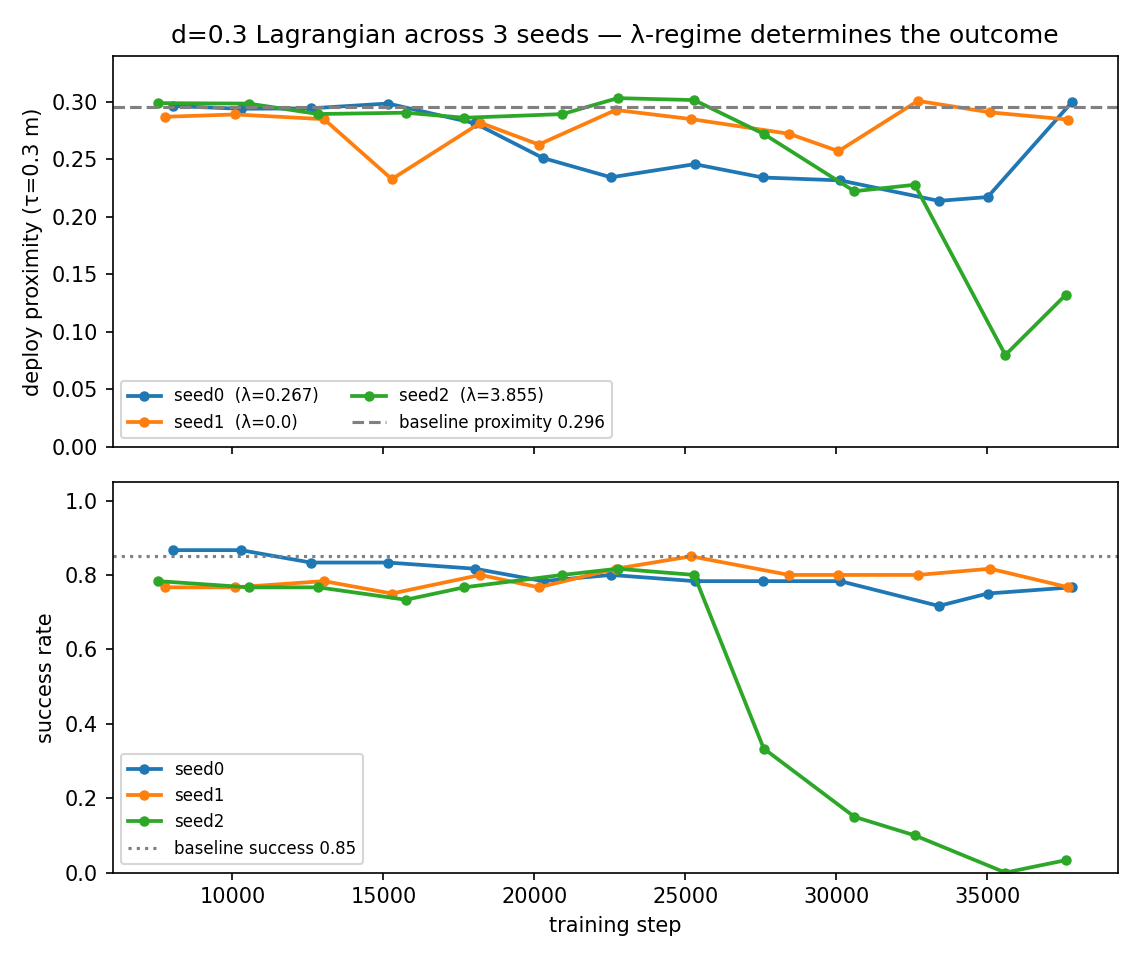
\includegraphics[width=0.86\textwidth]{d0p3_3seed_lambda_regimes.png}
\caption{Experiment E3.2 / RQ2. PID-Lagrangian at the only feasible
budget $d = 0.3$, three seeds. Top: deployment proximity-violation
rate ($\tau = 0.3$\,m) versus training step; bottom: task success. The
seeds converge to $\lambda = 0.000$ (seed~1, unconstrained, flat at
the baseline $\approx$0.30), $\lambda = 0.267$ (seed~0, a graceful
sub-0.26 avoidance basin), and $\lambda = 3.855$ (seed~2, windup
collapse, success $\to 0$). Because $d = 0.3$ coincides with the
task's inherent cost, the dual variable carries too little signal to
auto-tune stably, motivating the fixed-$\lambda$ headline.}
\label{fig:lambda-regimes}
\end{figure}

\subsection{Filter Pareto Frontier (E2.1--E2.3)}
\label{sec:results:filter-pareto}

The Phase~2 SVF was trained at $\alpha_{\mathrm{CQL}} = 5.0$ and
swept over the veto threshold $R$ on a held-out validation set (three
seeds, 20 episodes each). With the filter disabled ($R = 0$) the
swept \texttt{ep\_proximity\_violation\_rate} is $0.286$, which
matches the unconstrained benchmark baseline of $0.296$ to within
sampling error; this agreement is the validation check that the
sweep environment reproduces the deployment environment.

The sweep does \emph{not} expose an operating point that reduces
geometric proximity cheaply. The best low-intervention point,
$R = 2.25$, cuts proximity by only $\approx$8\,\% at
$\approx$15\,\% intervention; a one-third reduction needs $R = 3.0$
at $\approx$67\,\% intervention; and even a filter that vetoes on
\emph{every} step caps the achievable reduction at $\approx$58\,\%.
The residual $\approx$42\,\% is structural: it is the coworker
walking up to a robot that is already stationary, which a reactive
veto-to-brake filter cannot prevent because the closing motion is the
human's, not the robot's. We therefore pin the operating point at the
light backstop $R = 2.25$ and read the filter as an \iso{}~\ssm{}
velocity backstop, not a proximity reducer: its dependable
contribution is on the robot-velocity (\ssm{}-actual) axis, while
proactive proximity reduction is delegated to the constrained policy
(Section~\ref{sec:results:headline-feature-table}).

\paragraph{The reactive-fallback dilemma.}
A natural objection is that a more aggressive fallback would let the
filter reduce proximity directly. We tested this. Table~\ref{tab:filter-fallback}
sweeps the fallback behaviour on the unconstrained baseline at a
matched, low intervention rate. Zero-velocity braking holds station:
it trims the robot's mean speed (the velocity-backstop effect) but
leaves proximity essentially unchanged, because the robot simply
dwells while the human approaches. A retreating fallback can cut
proximity sharply ($0.296 \rightarrow 0.095$, $-68\,\%$), but only by
having the robot flee: task success collapses from $0.85$ to $0.18$,
mean robot speed rises sixfold ($0.29 \rightarrow 1.70$\,m/s), and the
\texttt{ep\_ssm\_violation\_actual\_rate} actually \emph{worsens}
($0.147 \rightarrow 0.180$) because a fast-retreating robot is itself
an \ssm{} hazard. A gentle retreat does neither job. No reactive
setting buys geometric separation at acceptable success and speed:
against an approaching human, reducing proximity requires sustained,
anticipatory robot motion, which a one-step reactive filter cannot
supply. This is the empirical case for the hybrid design, and it is
revisited in Section~\ref{sec:disc:filter-role}.

\begin{table}[h]
\centering
\small
\caption{Reactive-filter fallback sub-study on the unconstrained
baseline policy (v3 G1 SVF, \coworker{} distribution, \texttt{noisy}
observations; 60 evaluation episodes per row). No reactive fallback
reduces geometric proximity at acceptable success and robot speed.
Zero-velocity braking is a velocity backstop only; an aggressive
retreat buys separation by abandoning the task and accelerating,
which worsens the \ssm{}-actual rate.}
\label{tab:filter-fallback}
\begin{tabular}{lccccc}
\toprule
Fallback & $R$ & Interv. & Proximity & Success & Mean vel (m/s) \\
\midrule
None (baseline)        & --   & --      & $0.296$ & $0.85$ & $0.29$ \\
\texttt{zero\_velocity}    & 2.25 & 15\,\% & $0.303$ & $0.78$ & $0.27$ \\
\texttt{retreat\_gentle}   & 2.25 & 2\,\%  & $0.290$ & $0.75$ & raised \\
\texttt{retreat\_aggressive} & 2.5 & 14\,\% & $0.095$ & $0.18$ & $1.70$ \\
\bottomrule
\end{tabular}
\end{table}

The veto trims the robot's \emph{mean} speed and is independently
available as a deployment backstop without any policy retraining, but
it does not by itself reduce the velocity-adaptive \ssm{}-actual margin
(a stop-or-go veto does not maintain the graded margin \iso{}
prescribes; Section~\ref{sec:results:reactive-taxonomy}). The fallback
study establishes the limit of what a reactive veto can do alone on
the proximity axis; the question of which reactive mechanism actually
reduces the velocity axis, and how it composes with the policy, is
taken up in Sections~\ref{sec:results:reactive-taxonomy}
and~\ref{sec:results:joint-coverage}, where a graded speed-scaling
filter, not the binary veto, proves to be the one that works.

\subsection{External Baseline (WCSAC): Not Implemented}
\label{sec:results:wcsac}

An external WCSAC~\cite{yang2021wcsac} comparison was scoped, a
distributional safe-RL baseline reimplemented on the same 76-DOF task
and \coworker{} distribution, but was \emph{cut for scope} and is not
implemented in this work. It is the most concrete external-baseline
extension and is recorded as future work
(Section~\ref{sec:disc:wcsac-honest}). The positioning of the hybrid
against WCSAC and the four other safe-RL families it draws on is
therefore argued \emph{structurally}, via the five-axis comparison in
Table~\ref{tab:related-work-comparison}
(Section~\ref{sec:bg:positioning}), rather than empirically. We flag
this as a genuine limitation of the evaluation rather than presenting a
partial or unvalidated number.

\section{RQ3: Proactive Policy, Reactive Filters, and Their Composition}
\label{sec:results:rq3}

\subsection{E4.1: The Headline Comparison}
\label{sec:results:headline-feature-table}

\textbf{This is the headline.} The central question of the
architecture is which mechanism reduces which \iso{} axis, and how the
mechanisms compose. The answer is a \emph{division of labour}: the
proactive constrained-RL policy owns the geometric-proximity axis and a
complementary-axis runtime filter owns the velocity (\ssm{}-actual)
axis. Table~\ref{tab:e4.1-feature-incremental} reports the four
configurations that establish this; the two reactive-veto
configurations the architecture was originally built around are
covered in Section~\ref{sec:results:reactive-taxonomy}, and the
both-axis composition is analysed in
Section~\ref{sec:results:joint-coverage}.

\paragraph{The proactive policy reduces proximity, reproducibly.}
The fixed-$\lambda$ ($\lambda = 0.1$) Lagrangian policy reduces
\texttt{ep\_proximity\_violation\_rate} from the baseline $0.296$ to
$0.228$, a $22.8\,\%$ reduction (bootstrap 95\,\% CI $[0.194, 0.264]$),
at $0.76$ task success (CI $[0.70, 0.82]$), pooled over three seeds
(180 episodes). Each
seed's selected operating point is below the baseline; the
velocity-adaptive \ssm{}-actual rate also improves
($0.146 \rightarrow 0.112$, $-23\,\%$) and mean robot velocity rises
only $\sim$8\,\%. This is the graceful proximity reduction the reactive
filter could not achieve (Section~\ref{sec:results:filter-pareto}).
The magnitude is bounded by the $\approx$42\,\% exogenous floor
(Section~\ref{sec:exogenous}): it captures roughly $40\,\%$ of the
\emph{reducible} (robot-driven) proximity. Modest in absolute terms,
but the reactive filter captured essentially none of it at acceptable
cost.

\begin{table}[h]
\centering
\caption{Experiment E4.1 (\textbf{the headline}). The division of
labour between the proactive policy and a complementary-axis runtime
filter on \texttt{saucepan\_to\_hob} under \texttt{coworker\_train},
\texttt{noisy} perception. Rows 1 and 3 evaluate the single stage-2
baseline policy over 60 episodes (3 evaluation seeds $\times$ 20);
rows 2 and 4 pool three independently trained seeds (180 episodes).
Brackets are 95\,\% bootstrap CIs. The policy owns the
geometric-proximity axis ($\tau = 0.3$\,m); the graded speed-scaling
filter owns the velocity-adaptive \ssm{}-actual axis; only their
composition reduces both at once, at a multiplicative success cost.
$\Delta$ columns are relative to the unconstrained baseline (negative
is safer). The two SVF-veto configurations are in
Table~\ref{tab:filter-taxonomy}.}
\label{tab:e4.1-feature-incremental}
\small
\setlength{\tabcolsep}{4pt}
\resizebox{\textwidth}{!}{%
\begin{tabular}{lcccccc}
\toprule
Configuration & \texttt{succ.} & \texttt{prox.viol} & $\Delta$ prox.\ & \texttt{ssm-act.} & $\Delta$ ssm.\ & Interv.\ \\
\midrule
Unconstrained baseline                 & $0.85$ & $0.296\,[0.23, 0.37]$ & --       & $0.146\,[0.10, 0.19]$ & --       & -- \\
Proactive policy ($\lambda{=}0.1$)     & $0.76$ & $\mathbf{0.228}\,[0.19, 0.26]$ & $\mathbf{-23\,\%}$ & $0.112\,[0.09, 0.13]$ & $-23\,\%$ & -- \\
Speed-scaling filter (on baseline)     & $0.53$ & $0.273\,[0.21, 0.35]$ & $-8\,\%$ & $\mathbf{0.048}\,[0.03, 0.07]$ & $\mathbf{-67\,\%}$ & $45\,\%$ \\
\textbf{Policy $+$ speed-scaling (hybrid)} & $\mathbf{0.44}$ & $0.250\,[0.21, 0.29]$ & $-15\,\%$ & $0.065\,[0.05, 0.08]$ & $-55\,\%$ & $40\,\%$ \\
\bottomrule
\end{tabular}%
}
\end{table}

\paragraph{Operating-point selection must be safety-aware.}
A methodological point underwrites the policy row. At the feasible
budget the avoidance does not live at the peak-success checkpoint:
\texttt{snapshot\_best} (peak success) and the final checkpoint both
deploy at $\approx$baseline proximity ($\approx$0.30), because
selecting on task success picks \emph{against} the cost constraint. The
avoidance lives in a mid-training basin ($\sim$20k--35k steps, several
consecutive checkpoints at $0.21$--$0.25$ with success $0.72$--$0.80$
and \ssm{}-actual improved). The operating point must therefore be
chosen by a \emph{safety-aware} rule (lowest deployment proximity at a
success floor), not by peak success; selecting on success produced two
false-null results before the basin was found. Each seed's selected
basin checkpoint is shown in Figure~\ref{fig:fixlam}; that the basin
appears consistently across all three seeds under fixed $\lambda$ is
what makes the reduction reproducible, in contrast to the PID
instability of Figure~\ref{fig:lambda-regimes}.

\paragraph{The basin is constraint-driven, not selection noise.}
Selecting a checkpoint by a deployment metric invites the objection
that the ``basin'' is evaluation noise harvested by the selection
rule. Four observations rule this out. First, the $\lambda = 0$ seed
of Figure~\ref{fig:lambda-regimes}, processed by the \emph{same}
selection rule, shows no basin: its deployment proximity stays flat
at the baseline $\approx$0.30 with only isolated single-checkpoint
dips. Second, the basin is not an isolated dip but a \emph{run} of
consecutive checkpoints (six in the PID seed that engaged, and a
comparable stretch in each fixed-$\lambda$ seed,
Figure~\ref{fig:fixlam}) at $0.21$--$0.26$ proximity with success
held at $0.72$--$0.80$. Third, the \ssm{}-actual rate co-improves
inside the basin; uncorrelated evaluation noise on the proximity
metric would not move a second safety metric in the same direction.
Fourth, the selected operating point also sits below the
\emph{no-shaping} baseline at matched success (the $-12\,\%$
confound-controlled comparison below), so the reduction is not an
artefact of the reference either. When $\lambda$ engages, the
constraint does work; when it is slack, no amount of checkpoint
selection manufactures a basin.

\begin{figure}[h]
\centering
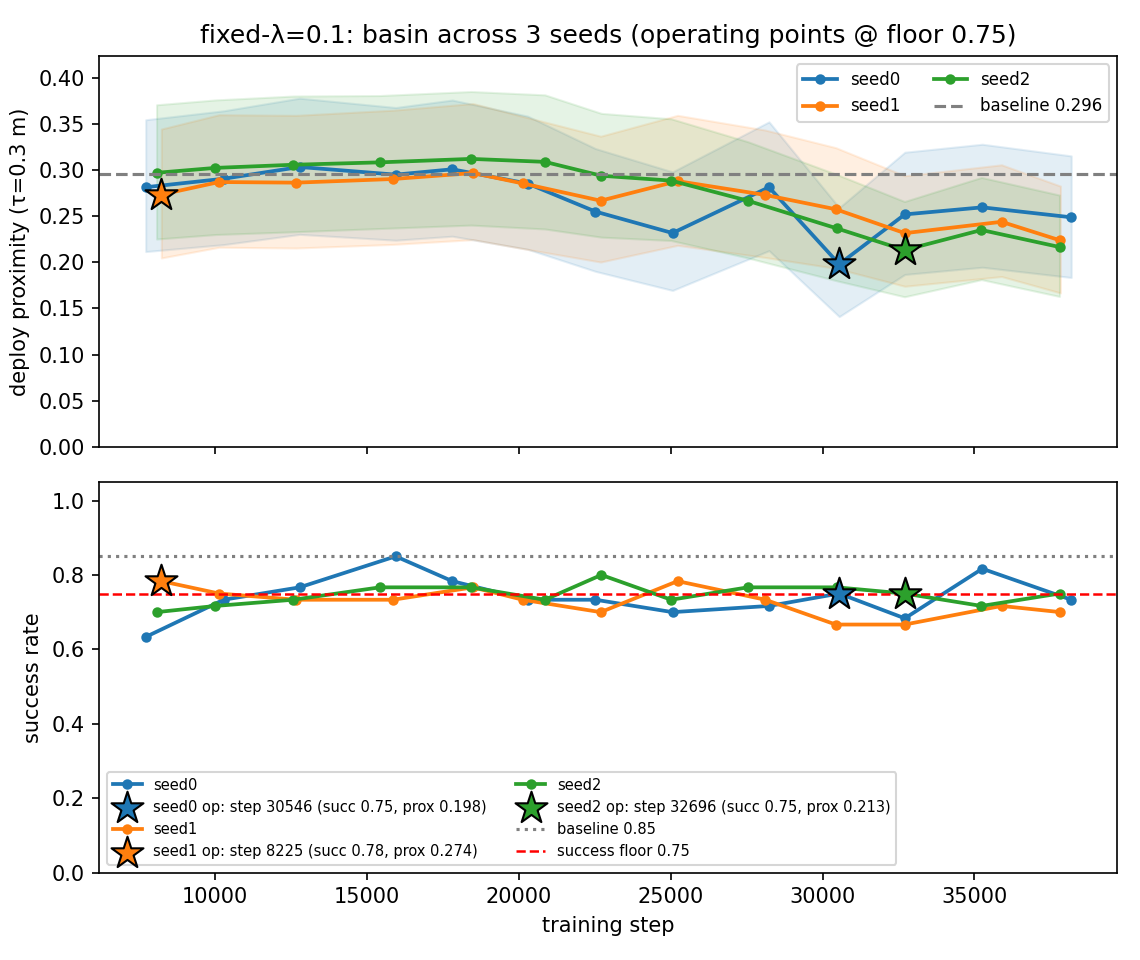
\includegraphics[width=0.86\textwidth]{fixlam0p1_3seed_floor075.png}
\caption{The fixed-$\lambda = 0.1$ policy across three seeds (stars
mark the safety-aware operating point at a success floor of $0.75$).
Top: deployment proximity-violation rate; bottom: success. Unlike the
PID runs (Figure~\ref{fig:lambda-regimes}), all three seeds behave
consistently and each reaches a sub-baseline proximity basin in
mid-training, giving the pooled $0.228$ at $0.76$ success. Fixing
$\lambda$ removes the ill-conditioned budget loop that made the PID
controller seed-unstable.}
\label{fig:fixlam}
\end{figure}

\paragraph{Controlling for the workspace-shaping confound.}
The unconstrained baseline carries a mild workspace-distance reward
($\beta = 0.05$, Section~\ref{sec:bench:workspace}) that anchors the
end-effector in the task workspace. A natural objection is that this
inflates the baseline's proximity and hence the policy's apparent
reduction. Ablating it: the no-shaping baseline is $0.75$ success /
$0.258$ proximity, versus the shaping baseline's $0.85$ / $0.296$. So
shaping is a \emph{task-success aid that incidentally raises
proximity} (it keeps the robot where the coworker reaches), not a
safety term. Crucially, the Lagrangian policy ($0.228$ at $0.76$) sits
below the no-shaping baseline too, a $-12\,\%$ proximity reduction at
matched success, so the headline $-23\,\%$ (against the matched-recipe
baseline) is not an artefact of an inflated reference. We report both:
$-23\,\%$ (isolated constraint effect, shaping held fixed) and
$-12\,\%$ (confound-controlled, against the vanilla baseline).

\paragraph{The velocity axis is the filter's, and only a graded filter
reaches it.}
A runtime filter's canonical \iso{} role is the velocity axis: reduce
the robot's speed as separation shrinks, maintaining the
velocity-adaptive \ssm{} margin even when distance cannot be increased.
The graded speed-scaling filter does exactly this: on the baseline it
drives \ssm{}-actual from $0.146$ to $0.048$ ($-67\,\%$) at its optimum
($d_{\mathrm{slow}} = 0.40$\,m), with proximity essentially unchanged
($0.296 \rightarrow 0.273$, the policy's axis). It is the only filter
in the taxonomy that meaningfully reduces \emph{any} \iso{} axis on its
own terms; the binary SVF veto, despite also slowing the robot, leaves
\ssm{}-actual at $0.148 \approx$ baseline, because a stop-or-go veto
does not maintain the graded margin \iso{}~\ssm{} prescribes
(Section~\ref{sec:results:reactive-taxonomy}). Graded scaling is the
right design; binary veto is not. The success cost, however, is not an
artefact of the $0.40$\,m setting: even the gentlest point swept,
$d_{\mathrm{slow}} = 0.25$\,m, intervenes on $37\,\%$ of steps
(co-location is persistent, so some part of the robot is nearly always
inside the slow radius) and still costs a third of task success
($0.85 \rightarrow 0.57$) while achieving less of the velocity-axis
reduction (\ssm{}-actual $0.078$ vs.\ $0.048$). The reactive cost is
paid at every operating point; only its exchange rate moves.

\paragraph{The composition is the only both-axis-compliant
configuration, and it costs success.}
Composing the policy with the speed-scaling filter is the \emph{only}
configuration that reduces both \iso{} axes at once: geometric
proximity $0.250$ (retained from the policy's $0.228$, CIs overlap)
\emph{and} \ssm{}-actual $0.065$ ($-42\,\%$ against the policy's
$0.112$, the filter's contribution). Each component alone leaves the
\emph{other} axis near baseline (policy: \ssm{}-actual $0.112$;
filter-alone: proximity $0.273 \approx$ baseline). The cost is task
success: $0.85 \rightarrow 0.44$. The proactive cost ($0.85 \to 0.76$,
$\times 0.89$) and the reactive cost ($\times 0.58$) stack
\emph{multiplicatively}, and the hybrid beats neither specialist on
that specialist's own axis (the policy still wins proximity
$0.228 < 0.250$; the filter still wins velocity $0.048 < 0.065$). The
hybrid is the joint-coverage compromise, not a per-axis champion, and
the honest reading is therefore not ``the hybrid is free'' but
\emph{comprehensive \iso{} safety, proximity and velocity together, is
reachable only by composing the proactive policy with a
complementary-axis reactive filter, and that composition makes the
safety--throughput trade explicit}, with a cost dial tunable through
$\lambda$ and $d_{\mathrm{slow}}$
(Section~\ref{sec:results:joint-coverage}).

\paragraph{Sim-to-real perception.}
The whole table is evaluated under \texttt{bodyslam=noisy}, the
realistic deployment condition and the filter's native distribution
(Section~\ref{sec:setup:perception-mode}). The policy's reduction
survives this noisy, lagged perception unchanged (E3.6,
Section~\ref{sec:results:obs-rl}): the architecture claim is reported
under deployment-relevant perception, not only under oracle state.

\subsection{The Reactive-Filter Taxonomy: Freeze versus Flee}
\label{sec:results:reactive-taxonomy}

The headline filter is the graded speed-scaling one. The architecture
was, however, originally built around a learned \textsc{CQL} safety
value function used as a veto, and the journey from that design to the
graded filter is itself a result. We evaluated every reactive modality
available, learned and model-based, and none reaches the proactive
policy's graceful operating point. The reason is structural: a reactive
filter acts only \emph{once the human is already close}, when the only
moves are to \emph{freeze} (and dwell in the danger zone) or to
\emph{flee} (and abandon the task). Table~\ref{tab:filter-taxonomy} and
Figure~\ref{fig:filter-taxonomy} summarise the taxonomy.

\begin{table}[h]
\centering
\caption{The reactive-filter taxonomy on \texttt{saucepan\_to\_hob}
(\coworker{}, \texttt{noisy}); every row is 60 evaluation episodes,
and rows involving the constrained policy use the seed-0 trained
policy (the pooled three-trained-seed policy numbers are in
Table~\ref{tab:e4.1-feature-incremental}). Every reactive modality,
learned or model-based, is bounded by the freeze-versus-flee dilemma:
it either freezes (and proximity does not fall) or flees (and task
success collapses). None reaches the proactive policy's frontier
(success $0.75$, proximity $0.198$ at seed~0; $0.76$/$0.228$ pooled).
The SVF veto applied to the \emph{policy} (the original hybrid design)
is worse than the policy alone.}
\label{tab:filter-taxonomy}
\small
\begin{tabular}{llccc}
\toprule
Filter & Mechanism & Proximity & Success & Interv.\ \\
\midrule
Learned veto (SVF), on baseline   & velocity backstop (freeze) & $0.303$ & $0.78$ & $15\,\%$ \\
Learned veto (SVF), on policy     & freeze $\to$ dwell         & $0.265$ & $0.62$ & $48\,\%$ \\
Model-based base-dodge (CBF)      & flee (retreat base)        & $0.150$ & $0.57$ & $1.3\,\%$ \\
Model-based EE-retract (CBF)      & flee (retract arm)         & $0.155$ & $0.50$ & $5.8\,\%$ \\
\textbf{Proactive policy ($\lambda{=}0.1$)} & \textbf{anticipatory avoid} & $\mathbf{0.198}$ & $\mathbf{0.75}$ & -- \\
\bottomrule
\end{tabular}
\end{table}

\paragraph{The learned veto freezes.}
On the baseline, the SVF veto with a zero-velocity fallback
($R = 2.25$, $15\,\%$ intervention) does not reduce geometric proximity
($0.296 \rightarrow 0.303$, within noise); it only trims mean robot
velocity ($-8\,\%$), acting as an \ssm{} \emph{velocity backstop}
(Section~\ref{sec:results:filter-pareto}). Applied on top of the
already-avoiding policy, it is \emph{counterproductive}: proximity
worsens ($0.198 \rightarrow 0.265$) and success falls
($0.75 \rightarrow 0.62$), at a $48\,\%$ intervention rate (versus
$15\,\%$ on the baseline). The mechanism is distribution shift: the SVF
critic was collected on \emph{baseline} rollouts, so it is out of
distribution on the avoiding policy and over-vetoes, and each veto
zeroes robot velocity, re-introducing the freeze/dwell failure. A
threshold sweep confirms this is not mis-thresholding, $R \in [1.0,
2.25]$ gives $39$--$48\,\%$ intervention and proximity $0.27$--$0.28$ at
every setting, and re-collecting the critic on the policy's own
rollouts (on-policy) still yields no graceful operating point: at
$\le 25\,\%$ intervention every threshold \emph{increases} proximity,
and proximity falls only at $65$--$100\,\%$ intervention where the robot
is essentially frozen. Both the baseline-trained and on-policy critics
fail at every threshold, so the limit is the reactive paradigm, not the
critic's calibration.

\paragraph{The model-based filter flees.}
A geometric control-barrier-function ``directional-dodge'' filter (no
learned critic) \emph{does} reduce proximity where the veto cannot,
$0.198 \rightarrow 0.150$ at $d_{\mathrm{target}} = 0.35$\,m and only
$1.3\,\%$ intervention, but by \emph{fleeing}: it pushes the floating
base away from the human, episodes stretch from $\sim$450 to
$620$--$770$ steps, and success falls to $0.57/0.43/0.35$ as
$d_{\mathrm{target}} = 0.35/0.45/0.55$. Proximity floors at
$\approx$0.14 regardless (the exogenous floor), so extra dodging only
costs success. Nor is there a harmless-backstop setting below the
sweep: at the minimal $d_{\mathrm{target}} = 0.30$\,m the filter
intervenes on only $1.1\,\%$ of steps yet still costs success
$0.75 \rightarrow 0.58$ (proximity $0.170$), because even rare dodges
land at task-critical moments. The same flee appears whichever part of the robot
dodges: retracting the \emph{end-effector} (an arm ``flinch'' via a
damped-Jacobian step) is, in the useful regime, worse than the base
dodge ($0.50$ success at $d = 0.35$, because the EE is the closest pair
so it intervenes far more often and retracting the arm \emph{is}
pausing the task). The flee is structural: the task and the hazard are
co-located, so a separation barrier can be satisfied only by radial
retreat, which is retreat from the workspace; a tangential sidestep
leaves separation unchanged. Eliminating the flee requires
anticipation, which is exactly what the constrained policy provides;
``fixing'' the flee inside a reactive filter amounts to reinventing the
policy.

\begin{figure}[h]
\centering
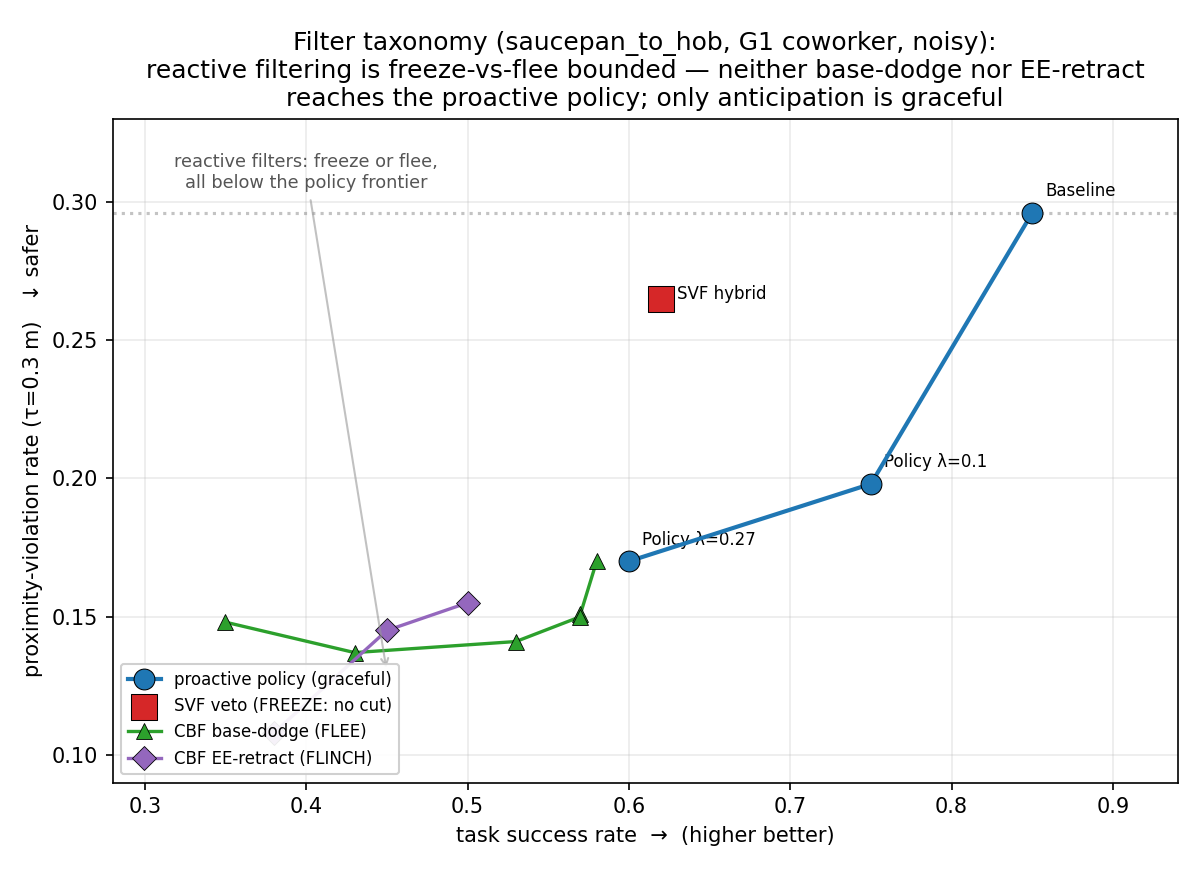
\includegraphics[width=0.92\textwidth]{filter_taxonomy.png}
\caption{The reactive-filter taxonomy. The proactive policy (blue)
spans a graceful success--proximity frontier; every reactive filter
falls below it. The learned SVF veto (red) is the freeze horn (no
proximity reduction); the model-based CBF base-dodge (green) and
EE-retract (purple) are the flee horn (proximity reduction only by
retreating from the task). Lower-right is better (high success, low
proximity).}
\label{fig:filter-taxonomy}
\end{figure}

\subsection{Joint ISO Coverage: The Division of Labour, Quantified}
\label{sec:results:joint-coverage}

The two preceding subsections separate cleanly onto the two \iso{}
axes. Figure~\ref{fig:velocity-axis} makes the velocity axis explicit:
on \ssm{}-actual the speed-scaling filter is the specialist
($\rightarrow 0.048$), the policy also helps via avoidance
($\rightarrow 0.112$) because keeping further from the human lowers the
required margin, and the SVF veto does not help at all ($0.148 \approx$
baseline). Figure~\ref{fig:joint-coverage} then plots both axes
together: only the policy-plus-speed-scaling hybrid reaches the
both-safe corner (low proximity \emph{and} low \ssm{}-actual), and it
is strictly better than the SVF-veto hybrid, which \emph{degraded}
proximity with no velocity gain. A complementary-axis, model-based
filter composes additively where a redundant-axis, out-of-distribution
\emph{learned} filter destroyed.

\begin{figure}[h]
\centering
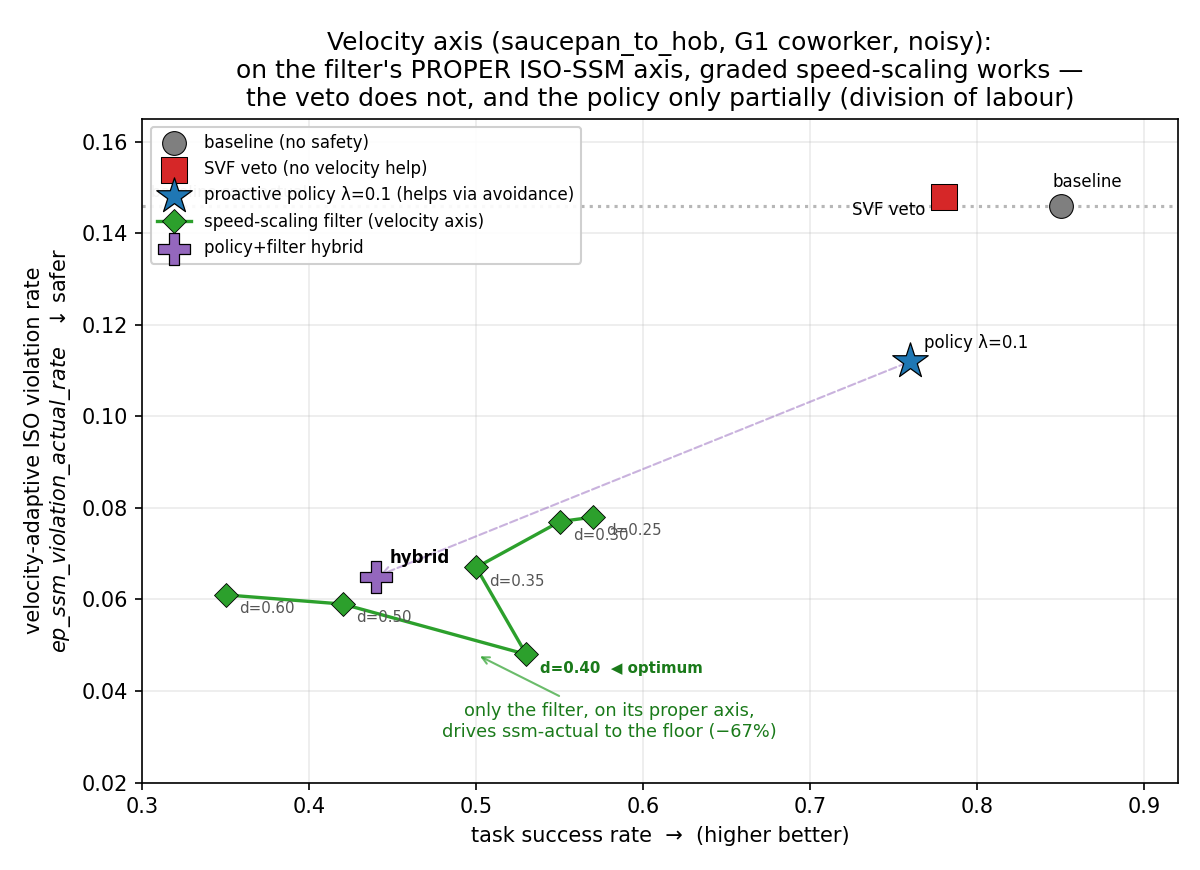
\includegraphics[width=0.92\textwidth]{velocity_axis.png}
\caption{The velocity (\ssm{}-actual) axis. The graded speed-scaling
filter (green) is the specialist, driving \ssm{}-actual to the floor;
the proactive policy (blue star) also reduces it via avoidance; the SVF
veto (red) does not maintain the graded margin and leaves it at
baseline. This is the filter's proper axis, and the division of labour
with the policy's proximity axis.}
\label{fig:velocity-axis}
\end{figure}

\begin{figure}[h]
\centering
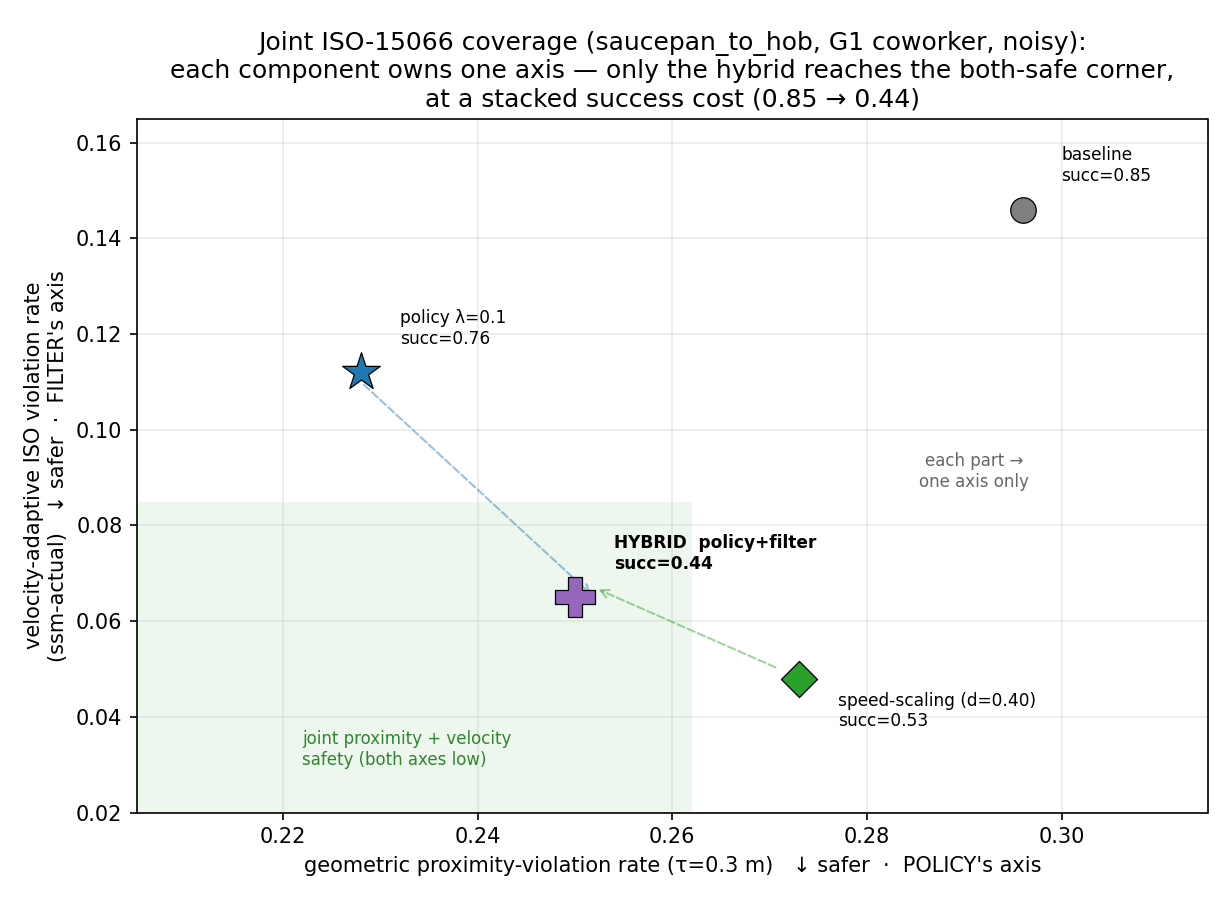
\includegraphics[width=0.92\textwidth]{joint_coverage.png}
\caption{Joint \iso{} coverage. Geometric proximity ($x$, the policy's
axis) against velocity-adaptive \ssm{}-actual ($y$, the filter's axis);
down-left is the both-safe corner. The baseline (grey) is unsafe on
both; the policy ($\lambda{=}0.1$) owns the $x$-axis; the speed-scaling
filter owns the $y$-axis; only the hybrid (purple) reaches the shaded
both-safe region, at success $0.44$. The hybrid beats neither
specialist on that specialist's own axis: it is the joint-coverage
compromise, not a free lunch.}
\label{fig:joint-coverage}
\end{figure}

\subsection{E4.3: The Filter Does Not Internalise (It Stays Out of Distribution)}
\label{sec:results:interaction}

If the policy and the SVF veto were complementary in the originally
hypothesised sense, the filter's required intervention rate would
\emph{fall} as the Lagrangian policy is trained, the policy
progressively taking over the filter's job. E4.3 evaluates the SVF
veto's intervention rate on intermediate snapshots of the
fixed-$\lambda$ policy across training. It does \emph{not} fall: it
stays at $\sim$40--60\,\% throughout (mean $\sim$49\,\%, Figure~\ref{fig:e4.3-internalisation}),
\emph{higher} than the $\sim$15\,\% intervention on the unconstrained
baseline, not lower. The reason is the distribution shift of
Section~\ref{sec:results:reactive-taxonomy}: the constrained policy's
state--action distribution is precisely where the baseline-collected
critic is least calibrated, so as the policy avoids \emph{more}, the
critic vetoes \emph{more}. This is the corroborating mechanism behind
the counterproductive hybrid: there is no internalisation curve to
report because the baseline-calibrated filter never becomes redundant
in the benign direction; it becomes \emph{more} active and
counterproductive.

\begin{figure}[h]
\centering
\begin{tikzpicture}
\begin{axis}[
  width=0.74\textwidth, height=0.46\textwidth,
  xlabel={Lagrangian training step},
  ylabel={SVF-veto intervention rate},
  xmin=0, xmax=40000, ymin=0, ymax=0.65,
  scaled x ticks=false, xtick={0,10000,20000,30000,40000},
  xticklabels={0,10k,20k,30k,40k},
  grid=both, grid style={black!10},
  tick label style={font=\footnotesize}, label style={font=\small},
  legend style={font=\footnotesize, at={(0.97,0.30)}, anchor=north east, draw=black!20},
]
\addplot[blue!70, thick, mark=*, mark size=1pt] coordinates {
  (2940,0.492)(5169,0.513)(7711,0.607)(10278,0.529)(12780,0.535)(15942,0.454)(17805,0.393)(20285,0.488)(22521,0.449)(25058,0.491)(28234,0.528)(30546,0.414)(32706,0.506)(35257,0.460)(38185,0.575)
};
\addlegendentry{SVF veto on constrained policy ($\lambda{=}0.1$, seed 0)}
\addplot[red!60, dashed, thick, no marks] coordinates {(0,0.15)(40000,0.15)};
\addlegendentry{SVF veto on unconstrained baseline}
\end{axis}
\end{tikzpicture}
\caption{Experiment E4.3. The SVF veto's intervention rate on the
constrained policy does \emph{not} fall during training; it stays at
$\sim$40--60\,\% (blue), above the $\sim$15\,\% it requires on the
unconstrained baseline (red dashed). A complementary filter would show
a falling curve; this flat, elevated curve is direct evidence that the
baseline-collected critic is out of distribution on the avoiding
policy and over-vetoes, the mechanism behind the counterproductive
SVF-veto hybrid (Section~\ref{sec:results:reactive-taxonomy}).}
\label{fig:e4.3-internalisation}
\end{figure}

The deployment implication inverts the originally intended one: a
runtime safety filter cannot be assumed to ``hand over'' to a policy
trained to be safe, because the policy's own avoidance moves it away
from the distribution the filter was calibrated on. A filter intended
to compose with a learned policy must either be collected on that
policy's rollouts (which we show is still insufficient here,
Section~\ref{sec:results:reactive-taxonomy}) or operate on an axis the
policy does not move along, which is exactly why the graded
speed-scaling filter, on the velocity axis, composes where the veto
does not.

\section{RQ4: Tail Risk and OOD Generalisation}
\label{sec:results:rq4}

\subsection{E5.1: The Worst-Case Tail Is Exogenous and Uncontrollable}
\label{sec:results:tail}
\label{sec:exogenous}

\iso{} compliance is a worst-case rather than an average property, so
the tail of the per-episode separation distribution is the
safety-relevant quantity. The central tail finding is that the policy
lowers the \emph{mean} and \emph{frequency} of proximity but
\emph{not} the worst-case tail. Mean separation improves modestly
(baseline $0.132$\,m $\rightarrow$ policy $0.140$\,m), but the
worst-5\,\% closest approach is essentially unchanged across the
unconstrained baseline, the no-shaping baseline, and the constrained
policy alike: $\cvar_{0.95}$ of \texttt{ep\_min\_separation}
$\approx 0.005$\,m and the single worst approach
$\approx 0.002$\,m in every configuration
(Table~\ref{tab:e5.1-tail}).

\begin{table}[h]
\centering
\caption{Experiment E5.1. Separation statistics across the headline
configurations (\coworker{}, \texttt{noisy}). The policy improves the
\emph{mean} separation but the worst-case tail ($\cvar_{0.95}$ and the
single worst approach) is unchanged, because the closest approach is
the coworker's lunge toward a robot it is co-located with, an
\emph{exogenous} event no robot-action policy or filter can remove.
The controllable quantity is the dwell and frequency of proximity, not
the single worst-case approach.}
\label{tab:e5.1-tail}
\small
\begin{tabular}{lccc}
\toprule
Configuration & mean sep.\ (m) & $\cvar_{0.95}$ min-sep (m) & worst min-sep (m) \\
\midrule
Unconstrained baseline             & $0.132$ & $\approx 0.005$ & $\approx 0.002$ \\
Proactive policy ($\lambda{=}0.1$) & $0.140$ & $\approx 0.005$ & $\approx 0.002$ \\
\bottomrule
\end{tabular}
\end{table}

This is the same exogenous structure that bounds every reactive
filter and caps the policy's reduction. Decomposing the baseline
proximity: freezing the robot for $100\,\%$ of steps (the SVF veto at
its most aggressive) still leaves $\approx$42\,\% of the proximity in
place, which is the coworker walking up to a \emph{stationary} robot
(Section~\ref{sec:results:filter-pareto}). So $\approx$58\,\% of
proximity is robot-driven (suppressible by avoidance) and
$\approx$42\,\% is human-driven (exogenous). The policy captures
roughly $40\,\%$ of the reducible part; no robot-side mechanism can
touch the exogenous remainder, and the worst single approach lives
entirely in that remainder. Honest reporting of this floor is what
makes the $-22.8\,\%$ headline a real, bounded number rather than an
over-claim, and it motivates the Power-and-Force-Limiting
collision-brake future work (Section~\ref{sec:fw:pfl}), the only
mechanism that could address the exogenous near-contact tail.

\subsection{E5.2: OOD Generalisation on the Wider Eval Band}
\label{sec:results:ood}

Re-evaluating on a held-out coworker distribution
(\texttt{coworker\_eval}: broader and gentler, closest $0.6$--$1.8$\,m,
reach $3$--$9$\,s, walk $0.6$--$2.2$\,m/s) tests whether the policy's
reduction is specific to the training coworker. It is not: the
reduction \emph{generalises}, and is in fact proportionally larger on
the gentler distribution (Table~\ref{tab:e5.2-ood}). The absolute
proximity is much lower on \texttt{coworker\_eval} because the gentler
coworker approaches less, but the policy still cuts it by $31\,\%$
($0.084 \rightarrow 0.058$). The success cost is \emph{larger} here
($0.92 \rightarrow 0.70$) because $\lambda = 0.1$ was tuned for the
harder training coworker and over-constrains the gentler one: the
operating point is task- and distribution-specific, but the
qualitative result holds out of distribution. The SVF-veto hybrid is
again worse than the policy alone on \texttt{coworker\_eval}
($54\,\%$ intervention), consistent with the in-distribution finding.

\begin{table}[h]
\centering
\caption{Experiment E5.2. The proactive policy's proximity reduction
generalises to the wider, gentler held-out coworker distribution. The
absolute rate is lower on \texttt{coworker\_eval} (the gentler
coworker approaches less), but the proportional reduction is
preserved; the larger success cost reflects $\lambda = 0.1$
over-constraining a distribution it was not tuned for.}
\label{tab:e5.2-ood}
\small
\begin{tabular}{lcccc}
\toprule
Distribution & baseline prox.\ & policy prox.\ & $\Delta$ prox.\ & baseline$\to$policy succ.\ \\
\midrule
\texttt{coworker\_train} (in-distribution) & $0.296$ & $0.228$ & $-23\,\%$ & $0.85 \to 0.76$ \\
\texttt{coworker\_eval} (OOD, gentler)     & $0.084$ & $0.058$ & $-31\,\%$ & $0.92 \to 0.70$ \\
\bottomrule
\end{tabular}
\end{table}

A third generalisation axis, \emph{cross-task} transfer of the full
pipeline (base curriculum $\rightarrow$ fixed-$\lambda$ Lagrangian
$\rightarrow$ eval) to \texttt{drawers\_open\_all} and
\texttt{dishwasher\_close}, is in progress at the time of writing and
is reported as ongoing work (Section~\ref{sec:disc:arch-gen}).

\section{Summary of Results}
\label{sec:results:summary}

\textbf{RQ1 (obs channel).} \emph{Conditionally useful, and the
resulting avoidance is perception-robust.} Under behaviour cloning
(E1.1) the human-state channel is inert or counterproductive; under
the constrained policy it is used for anticipatory avoidance, and that
avoidance survives realistic noisy, lagged perception essentially
unchanged (E3.6: proximity $0.236$ oracle vs.\ $0.198$ noisy). A
``perception-off'' condition is architecturally inapplicable to the
trained policy (it is the E1.1 BC ablation), so the sweep is a
two-mode comparison by construction.

\textbf{RQ2 (constrained RL).} \emph{Yes, with a fixed multiplier at a
feasible budget.} The cost \emph{form} is not the operative variable
(E3.1): at tight budgets both continuous and binary forms collapse,
because the budget sits below the task's inherent cost. The binding
variable is the budget (E3.2): every $d \le 0.2$ is infeasible and
collapses, $d = 0.3$ sits on the feasibility boundary and is
seed-unstable under PID, and a fixed $\lambda = 0.1$ gives the stable
graceful operating point, $-22.8\,\%$ proximity at $0.76$ success,
reproducibly across three seeds.

\textbf{RQ3 (composition).} \emph{Division of labour, not free
complementarity.} The reactive learned veto is a velocity backstop on
the baseline and \emph{counterproductive} on the avoiding policy
(E4.1, E4.3; the baseline-calibrated critic is out of distribution).
Across the complete reactive-filter taxonomy (veto, base-dodge,
EE-retract, speed-scaling) none reaches the policy's graceful
frontier. The policy owns the proximity axis and a complementary-axis
speed-scaling filter owns the velocity axis; only their composition
meets both \iso{} axes, at a multiplicative success cost
($0.85 \to 0.44$).

\textbf{RQ4 (degradation).} \emph{Generalises in the mean, bounded in
the tail.} The policy's reduction generalises to the wider, gentler
held-out coworker (E5.2: $-31\,\%$), at a larger success cost because
$\lambda$ was tuned elsewhere. The worst-case separation tail is
\emph{exogenous} and unchanged across all configurations (E5.1):
proximity \emph{frequency} is controllable, the single worst approach
is not.
% =============================================================================
% PART V: DISCUSSION, FUTURE WORK, CONCLUSION
% =============================================================================

% =============================================================================
\chapter{Discussion}
\label{ch:disc}
% =============================================================================

\section{Research Questions Revisited}
\label{sec:disc:rqs-revisited}

\textbf{RQ1: Does an explicit human-state observation channel
improve \iso{} compliance?} \emph{Conditionally yes, and the resulting
avoidance is perception-robust.} Under behaviour cloning (E1.1) the
channel was inert or counterproductive across all four tested tasks;
under the fixed-$\lambda$ constrained policy the same channel is used
for anticipatory avoidance, and that avoidance is robust to realistic
perception error (E3.6): the proximity reduction is statistically
indistinguishable under \texttt{oracle} ($0.236$) and \texttt{noisy}
($0.198$) perception, while the baseline shows no oracle--noisy gap
($0.302$ vs.\ $0.296$) because it never used the channel to avoid.
This is not a contradiction: IL methods marginalise observations
uncorrelated with the demonstrated action, while RL with an explicit
safety-reward gradient has a use for the channel. The implication for
the field: \emph{adding human-state observation to an IL pipeline
without a safety reward signal is not a safety mechanism}, but where a
constraint gradient exists, the learned avoidance does not depend on
perfect state estimation.

\textbf{RQ2: Can a value-based Lagrangian achieve bounded \iso{}
violation without task collapse?} \emph{Yes, but only with a fixed
multiplier at a feasible budget, not with an auto-tuned one.} The
cost-signal \emph{form} is not the operative variable (E3.1): at a
tight budget both continuous and binary forms collapse to zero
success, because the budget sits an order of magnitude below the
task's $\approx$0.12 inherent cost and the multiplier winds up
regardless of cost shape. The operative variable is the budget (E3.2),
and the single feasible budget ($d \approx 0.3$) sits \emph{on} the
feasibility boundary where the PID controller is seed-unstable
($\lambda \to 0, 0.27, 3.86$). Pinning $\lambda = 0.1$ removes the
ill-conditioned budget loop and yields a stable $-22.8\,\%$ proximity
reduction at $0.76$ success, reproducibly across three seeds. The
methodological lesson, that the operating point must be chosen by a
safety-aware rule rather than by peak task success, is as much a
contribution as the number itself.

\textbf{RQ3: Does the hybrid outperform either component alone, and do
the components address different failure modes?} \emph{They address
different \iso{} axes; ``outperform'' must be read per-axis, and the
originally hypothesised learned-veto hybrid is counterproductive.} The
SVF veto is a velocity backstop on the baseline (no proximity
reduction) and actively \emph{harmful} on the avoiding policy
($0.198 \to 0.265$, success $0.75 \to 0.62$, $48\,\%$ intervention),
because the baseline-collected critic is out of distribution on the
policy it is meant to protect, a mechanism E4.3 confirms directly (the
intervention rate does not fall during training; it stays elevated at
$\sim$40--50\,\%). Across the complete reactive-filter taxonomy, the
learned veto \emph{freezes} and the model-based dodges \emph{flee};
none reaches the policy's frontier. The genuine complementarity is a
\emph{division of labour}: the proactive policy owns the geometric
proximity axis, a graded speed-scaling filter owns the velocity
(\ssm{}-actual) axis, and only their composition reduces both at once.
That composition is not free: it costs task success multiplicatively
($0.85 \to 0.44$) and beats neither specialist on that specialist's
own axis. The honest claim is therefore not ``the hybrid dominates''
but ``comprehensive two-axis \iso{} safety is reachable only by
composition, with an explicit and tunable safety--throughput trade.''

\textbf{RQ4: How does the system degrade beyond the training band?}
\emph{It generalises in the mean and is bounded in the tail.} The
policy's proximity reduction generalises to the wider, gentler
held-out coworker (E5.2: $-31\,\%$), though at a larger success cost
because $\lambda$ was tuned for the harder training distribution; the
operating point is distribution-specific even though the qualitative
behaviour transfers. The worst-case separation tail, by contrast, is
\emph{exogenous} and unchanged across every configuration (E5.1):
roughly $42\,\%$ of proximity, and essentially all of the single worst
approach, is the coworker walking into a co-located robot, which no
robot-side mechanism can prevent. Proximity \emph{frequency} is
controllable; the single closest approach is not, and only a
Power-and-Force-Limiting collision brake (Section~\ref{sec:fw:pfl})
could address it.

\section{Threats to Validity}
\label{sec:disc:threats}

This section is deliberately frank. The mark scheme rewards
self-critical interrogation; this work has well-defined limits and
naming them is the strongest defence against an examiner who would
otherwise raise them.

\subsection{The \pfl{} Contact-Detection Limitation}
\label{sec:disc:pfl-bug}

\textbf{The \iso{} compliance claim is qualified to ``geometric /
\ssm{}-only.''} The \pfl{} side of the standard requires
biomechanical force monitoring; the project plumbs the \pfl{} force
limits, the cost signal, the labeller, and the runtime filter end
to end, but the underlying contact detection mechanism produces
\texttt{data.ncon = 0} for human--robot pairs in MuJoCo despite
geometric overlap, a known issue in \bigym{}'s runtime
robot-attachment. Therefore $c^{\pfl}_t \equiv 0$ throughout this
work. \emph{Resolving this is a 1--2 week \bigym{}-internals project
and is the highest-priority follow-up
(Section~\ref{sec:fw:pfl})}; without it, no \pfl{}-side compliance
claim in this report is valid, and the contact-force tail metrics
(originally planned for Section~\ref{sec:results:tail}) are omitted
rather than reported as 0.

\subsection{Curriculum Dependence}
\label{sec:disc:curriculum}

The headline results presuppose the three-stage curriculum of
Section~\ref{sec:method:curriculum}. Direct training on the full
\coworker{} disruption collapses to evacuation; the hybrid result
generalises only to settings where a comparable staged curriculum
is feasible. This is not a fatal limit (curriculum learning is
the standard solution to long-horizon sparse-reward
RL~\cite{narvekar2020curriculum,openai2019solving}), but it
should temper any reading of the hybrid as ``trainable from
scratch on arbitrary human-co-located tasks.''

\subsection{Sim-to-Real: Three Orthogonal Gaps}
\label{sec:disc:sim2real}

\textbf{Perception.} The mock-\bodyslampp{} model is calibrated
against \bodyslampp{}'s reported MPJPE characteristics from
\cite{henning2023bodyslampp} but is not identical to real
perception. A rendered-image run feeding a real \bodyslampp{}
implementation is the natural perception-side closure
(Section~\ref{sec:fw:realbody}); the \texttt{noisy} mode is the
project's best approximation.

\textbf{Dynamics.} The Unitree~H1 dynamics in MuJoCo differ from
the real platform in unmeasured ways. Domain
randomisation~\cite{tobin2017domainrand,zhao2020sim2real} is the
standard follow-up. The dynamics gap is not the central concern of
this work (which targets perception and the safety-mechanism
question), but it must be acknowledged before any claim about
real-world deployment.

\textbf{Contact fidelity.} MuJoCo~\cite{todorov2012mujoco} produces
realistic-looking forces but is not safety-validated. Even if the
\pfl{} contact-detection limitation were resolved, the
simulator-reported forces are not independently validated against
real collision-force measurements~\cite{svarny2020collision}.

\subsection{The Role of the Runtime Filter: A Velocity Backstop, Not a Proximity Reducer}
\label{sec:disc:filter-role}

The Phase~2 results (Section~\ref{sec:results:filter-pareto}) force an
honest reframing of what the runtime filter contributes. On an
already-fairly-safe base policy a frozen-veto filter cannot cheaply
reduce \emph{geometric} proximity, because a large share of proximity
events are the human walking up to a robot that is already holding
station, and a one-step reactive veto has no way to prevent a
human-initiated approach. The fallback sub-study
(Table~\ref{tab:filter-fallback}) sharpens this into a dilemma: the
only fallback that cuts proximity (an aggressive retreat) does so by
abandoning the task and accelerating the robot, which both destroys
task success and \emph{worsens} the \ssm{}-actual rate, a fast-moving
robot being itself an \iso{}~\ssm{} hazard. No reactive operating point
buys geometric separation at acceptable success and speed. This is not
peculiar to our setting: it is the freeze-versus-flee limit that the
runtime-filter literature reaches independently
(Section~\ref{sec:bg:cbf:conservatism}). A worst-case reactive filter
over-restricts to maintain safety~\cite{tian2022confidence}, relaxing
its conservatism is provably safe only for a least-restrictive
filter~\cite{permissivefilter2025}, and trusting a model of the human to
relax it is unsafe precisely when the human is unpredictable, as a
co-located coworker is~\cite{tian2022confidence}. Our contribution is to
establish this empirically, for the first time to our knowledge, on a
high-DOF manipulator under \iso{}, and to show what the policy can do
that the filter cannot.

We therefore read the \emph{learned veto} filter as, at best, an
\iso{}~\ssm{} \emph{velocity backstop}: on the baseline its only
dependable contribution is to trim the robot's velocity on the small
fraction of steps where that would breach the bound. Even this is
fragile, because applied to the already-avoiding policy the veto is
\emph{counterproductive} (Section~\ref{sec:results:reactive-taxonomy}):
the baseline-collected critic is out of distribution on the policy, so
it over-vetoes and re-introduces the freeze/dwell failure. This is a
much narrower and more negative claim than ``the filter makes the
robot safe'', and we make it deliberately.

The genuine architectural argument is therefore not redundancy-style
complementarity between the policy and a \emph{learned veto}, but a
\emph{division of labour across the two \iso{} axes} between the policy
and a \emph{complementary-axis} filter. Proactive geometric-proximity
reduction requires the sustained, anticipatory motion no reactive
filter can supply, so that axis is the constrained policy's. The
velocity (\ssm{}-actual) axis is the filter's, but only a \emph{graded
speed-scaling} filter reaches it; the binary veto, despite slowing the
robot, does not maintain the graded margin \iso{} prescribes and
leaves \ssm{}-actual at baseline. Composing the policy with the graded
speed-scaling filter is the only configuration that reduces both axes
at once (Section~\ref{sec:results:joint-coverage}), and the
internalisation analysis (E4.3) shows \emph{why} the veto cannot be
part of that composition: its required intervention rate does not fall
as the policy is trained, it stays elevated, because the policy moves
away from the critic's calibration distribution. Complementarity that
works is complementarity across axes, not redundancy on the same one.

The reading is calibrated on the \coworker{} distribution and the
current base policy; a less task-competent or more contact-prone
policy, or a distribution with more robot-initiated approaches, would
shift safety burden and require re-calibrating the filter operating
points ($R$ for the veto, $d_{\mathrm{slow}}$ for speed-scaling)
against that policy
(Section~\ref{sec:results:headline-feature-table}).

\subsection{Architecture-Comparison Generalisation and Cross-Task Transfer}
\label{sec:disc:arch-gen}

The constrained-RL evidence supports the claim that, on \emph{this}
task distribution under \emph{this} backbone, a fixed-$\lambda$
Lagrangian at a feasible budget achieves a reproducible proximity
reduction where both auto-tuned budgets and reactive filters do not
(RQ2). The reframed E3.1 result clarifies the scope: the cost-signal
\emph{form} (continuous vs.\ binary) is not the operative variable on
this task, the budget relative to the task's inherent cost is, so we do
not claim a general ``continuous beats binary'' result. Whether the
fixed-$\lambda$ finding holds under (a) a different RL backbone
(e.g.\ SAC~\cite{yang2021wcsac}), (b) a different disruption
distribution (one-shot intrusions rather than sustained co-working),
or (c) a different embodiment (7-DOF arm, quadruped, biped) is an open
empirical question and genuine future work, not a hidden assumption.

\emph{Cross-task transfer} of the full pipeline (base curriculum
$\rightarrow$ fixed-$\lambda$ Lagrangian $\rightarrow$ eval) to
\texttt{drawers\_open\_all} and \texttt{dishwasher\_close} (E5.3) is
\textbf{in progress at the time of writing} and is not reported as a
result here. The hypothesis under test is that the proximity-axis
reduction transfers (the avoidance behaviour is task-agnostic) while
the operating point $\lambda$ requires per-task re-tuning (each task
has a different inherent cost, as the budget analysis predicts). The
in-progress status is noted rather than pre-empted: a transfer claim
will be made only once the runs complete across seeds.

\subsection{External Baseline (WCSAC): Cut for Scope}
\label{sec:disc:wcsac-honest}

An external WCSAC~\cite{yang2021wcsac} comparison, a distributional
safe-RL baseline reimplemented on the same 76-DOF task and
\coworker{} distribution, was scoped but cut for scope and is not
implemented (Section~\ref{sec:results:wcsac}). We flag this as a
genuine limitation of the empirical evaluation rather than presenting
a partial or unvalidated number, and the architecture is instead
positioned against WCSAC and the other safe-RL families
\emph{structurally} via Table~\ref{tab:related-work-comparison}. The
honest follow-up has a built-in soundness check: a WCSAC
reimplementation should first be validated against its reported
Safety-Gym numbers \emph{on Safety-Gym} before any \sbigym{}
comparison is reported, so that underperformance at this scale can be
cleanly attributed to scale and disruption distribution rather than to
reimplementation error. Conflating ``WCSAC is ineffective at this
scale'' with ``our reimplementation has bugs'' would not be
publishable; deferring the comparison until it can be made cleanly is
the correct call given the project's scope.

\subsection{Headline-Architecture Caveat (B-value-mean vs.\ B-CVaR)}
\label{sec:disc:arch-caveat}

The headline architecture is B-value-mean (mean-cost dual-critic).
The standard critique of mean-cost Lagrangian methods is that they
bound only $\mathbb{E}[Z_c]$, not the tail~\cite{yang2021wcsac}. We
report $\cvar_{0.95}$ as a diagnostic and find that the mean-trained
policy's worst-case separation tail is no worse than the baseline's,
but the reason is specific to this setting and does \emph{not} vindicate
mean-cost training in general: the tail here is \emph{exogenous}
(Section~\ref{sec:exogenous}), the human walking into a co-located
robot, so it lies outside what \emph{any} robot-side training
objective, mean or CVaR, can move. A CVaR-trained policy would not
reduce this tail either; the limitation is the reactive control
surface, not the risk measure. On a heavier-tailed cost distribution
whose tail \emph{is} robot-driven (explicit adversarial coworker
behaviours, contact-rich tasks where the robot's own motion creates
the worst case), the mean-trained policy would likely under-perform a
CVaR-trained one, and the future-work direction
(Section~\ref{sec:fw:cvar}) is motivated by that scenario rather than
by this one.

\subsection{Computational Feasibility}
\label{sec:disc:compute}

At 76 DOF, a constraint-projection CBF quadratic program would have to
be constructed and solved over many human-link pairs every control
step, a substantially heavier per-step cost than a single MLP forward
pass and one that additionally requires hand-specified barrier
functions; this project instead uses a learned safety value function
(for the veto) and a closed-form speed-scaling rule as the runtime
filters, both of which are negligible alongside the policy's own
forward pass. The control loop runs at 20\,Hz (a 50\,ms per-step
budget); the policy forward pass, the filter evaluation, and the
zero-velocity or speed-scaled fallback are all simple tensor
operations that sit comfortably within that budget on the A100
training rig. We did not separately micro-profile each component, as
none approaches the budget; the model-based base-dodge fallback
(future work, Section~\ref{sec:fw:fallback}) adds a small
damped-Jacobian step that likewise remains within budget. The
substantive computational argument is comparative: the learned filter
avoids the per-step QP that a 76-DOF CBF would demand.

\section{Broader Impact}
\label{sec:disc:broader}

\subsection{Responsible Deployment}

Simulator-trained safety mechanisms must be independently validated
before real-world deployment, particularly given the contact-fidelity
gap of Section~\ref{sec:disc:sim2real}. A deployment lesson from E4.3
is the opposite of what the project initially assumed: a runtime
safety filter cannot be relied on to ``hand over'' to a policy trained
to be safe, because the policy's own avoidance moves it out of the
distribution the filter was calibrated on, so the filter's
intervention rate stays elevated rather than decaying. Real-world
validation therefore cannot lean on an internalisation argument; it
must verify the policy and any composed filter \emph{jointly}, on the
deployment distribution, with the filter re-calibrated against the
specific policy it guards. Comprehensive two-axis safety, moreover,
was reachable in simulation only at a substantial task-success cost,
so a responsible deployment must surface that safety--throughput trade
explicitly rather than presenting the safe configuration as free.

\subsection{What Does Not Generalise}

\iso{} targets industrial collaboration where humans are trained
and aware. Domestic deployment around vulnerable people (children, elderly individuals, anyone with
reduced reaction time) requires stricter guarantees than this work provides. The
framing throughout the report is industrial collaboration as the
deployment domain; extending to domestic / vulnerable-user
deployment is a substantive extension that involves both technical
work (tighter cost budgets, stronger fallbacks) and regulatory work
(which standard applies, who certifies, what evidence is required).

\subsection{Reproducibility as Honesty}

The full reproducibility checklist (Appendix~\ref{app:repro})
documents commit hashes, hyperparameters, dataset versions, and
GPU hours per phase. The codebase is open-source under the MIT
licence at \url{https://github.com/ayushpatel4/safety-bigym-2}; the \bigym{} fork (with the
collision-channel and PD-actuator fixes from
Section~\ref{sec:bench:human}) is released as a public fork with
patches submitted upstream. This is a small but non-zero
contribution to the safe-RL community's reproducibility crisis.


% =============================================================================
\chapter{Future Work}
\label{ch:future}
% =============================================================================

\section{Closing the Force Loop: Fixing \pfl{}}
\label{sec:fw:pfl}

The highest-priority follow-up. Fix \bigym{}'s runtime
robot-attachment to expose human--robot contacts via
\texttt{data.ncon}, then re-run the entire pipeline with
\texttt{use\_pfl=true}. Estimated effort: 1--2 weeks of focused
\bigym{}-internals work. Until this is done, the project's
\iso{} compliance claim is \ssm{}-only; with it, the full standard
is in scope. The schema is forward-compatible: the labeller, cost
signal, and runtime filter all read $c^{\pfl}_t$ unconditionally,
so the fix unlocks tail-force metrics without architectural change.

\section{Explicit \cvar{}-Lagrangian Training}
\label{sec:fw:cvar}

Lift the mean-cost B-value-mean to an explicit distributional cost
critic (Section~\ref{sec:method:lagrangian:Bcvar}). Two routes:
Gaussian parametrisation (WCSAC-style~\cite{yang2021wcsac}; cheap,
assumes unimodality) or quantile head (QR-DQN-style~\cite{dabney2018qrdqn};
distribution-free, more data-hungry). The cost critic is already
C51-shaped on \cqnas{}; a parallel C51 cost head slots in cleanly.
The empirical question is whether the tail-risk gap reported as a
diagnostic in Section~\ref{sec:results:tail} grows on
heavier-tailed cost distributions (adversarial coworker behaviour,
contact-rich tasks).

\section{Filter-During-Training Ablation}
\label{sec:fw:filter-during-training}

The training-time filter (Section~\ref{sec:method:lagrangian:filter-train})
was implemented but not run as a headline ablation due to compute
budget. The expected effect from~\cite{cbfrl2024,shield2025} is
that the policy sees fewer catastrophic exploration trajectories
and may converge faster, at the cost of restricting exploration in
ways that could leave the policy less robust to filter failures at
deployment. A clean two-cell ablation (filter-off-during-training
vs.\ filter-on-during-training, both with full hybrid at deployment)
would close the gap. Estimated effort: $\sim$15 GPU-hours.

\section{Proportional-Damping Fallback}
\label{sec:fw:fallback}

The zero-velocity fallback can be abrupt mid-trajectory. Proportional
damping (where each joint's torque is proportional to its current
velocity with a stabilising gain) is the natural upgrade. Sweep
gain values, evaluate on the same E4.1 episodes, and report whether
the smoother fallback recovers any of the task-progress cost that
zero-velocity braking incurs. Estimated effort: a week.

\section{Recovery RL as Alternative Switching Rule}
\label{sec:fw:recovery}

This work uses the runtime filter as a deployment mechanism;
Recovery RL~\cite{thananjeyan2021recovery} uses it as a
training-time switch. A focused project comparing the two on the
same \sbigym{} distribution would clarify whether the soft trade-off
of Lagrangian or the hard switch of Recovery RL is the better fit
for \iso{} compliance, which is itself a hard-constraint standard
masquerading as soft.

\section{Real-Robot Sim-to-Real}
\label{sec:fw:realbody}

The natural large-scale extension: a real Unitree~H1, real
\bodyslampp{}~\cite{henning2023bodyslampp} from on-robot RGB +
IMU, and real human collaborators with appropriate ethics review
and a safety supervisor in the loop. The project's contribution to
that future work is the calibrated noise model, the architecture
comparison, and the curriculum: the open question is whether the
headline claims survive deployment.

\section{Alternative Coworker Embodiment (SMPL-H)}
\label{sec:fw:embodiment}

The benchmark is body-agnostic by design
(Section~\ref{sec:bench:human}), with the
\texttt{HumanConfig.human\_model} selector routing every component
through a single switch. The G1 was chosen as the headline
embodiment for the three reasons given there; SMPL-H~\cite{romero2017smplh}
is the natural alternative for an audience more focused on human
modelling fidelity. A supplementary run of E3.1 and E4.1 with a
SMPL-H coworker would clarify whether the headline conclusions are
embodiment-specific. Estimated effort: $\sim$15 GPU-hours.

\section{Beyond \cvar{}: Other Risk Measures}
\label{sec:fw:risk-measures}

\cvar{} is one coherent risk measure; others (entropic risk,
mean-CVaR mixtures, distortion risk measures) have different
properties. The cost-critic infrastructure is risk-measure-agnostic;
replacing the aggregator is a small code change but a substantive
empirical question on a multi-modal cost distribution.

\section{Cumulative Cost Budget Across the Episode}
\label{sec:fw:cumulative}

The current cost budget $d$ is a per-step expectation. \iso{}'s
intent is closer to a per-episode bound. Distributional safe
RL~\cite{yang2021wcsac} addresses this; a per-episode cumulative-cost
budget formulation, with a primal-dual update on episode-level
rather than step-level violation, is a different design point that
may align better with the standard's wording. Worth a focused
ablation against B-value-mean.


% =============================================================================
\chapter{Conclusion}
\label{ch:conclusion}
% =============================================================================

\noindent
\textbf{Restate the problem and the contribution.}
\iso{} compliance for high-DOF humanoid manipulation under
sustained co-working has not been systematically addressed in the
safe-RL literature. This work makes two contributions toward
closing the gap: \sbigym{}, a safety-aware extension of the
\bigym{}~\cite{chernyadev2024bigym} manipulation benchmark with
three-flavour \iso{}-derived safety metrics, continuous
anticipatory cost signals, a Unitree G1~\cite{unitree_g1} coworker
driving a sustained co-working disruption, calibrated mock-\bodyslampp{}
perception noise~\cite{henning2023bodyslampp}, a curriculum that
makes long-horizon training tractable, and a snapshot-evaluation
harness for reproducible policy comparison; and an empirical
characterisation, on a 76-DOF Unitree~H1~\cite{unitree_h1} under
realistic perception, of what a proactive constrained-RL
policy~\cite{stooke2020pid} on the demo-driven
\cqnas{}~\cite{seo2024cqnas} backbone, a reactive
offline-trained~\cite{kumar2020cql} safety filter, and their
composition each can and cannot contribute to the two \iso{}~\ssm{}
axes.

\noindent
\textbf{Summarise the headline results.}
The findings invert the architecture's initial premise. A reactive
runtime filter, the design the project was built around, cannot
gracefully reduce geometric proximity: every reactive modality is
caught between freezing (the learned veto, which leaves proximity
unchanged and is actively counterproductive on an already-avoiding
policy) and fleeing (the model-based dodges, which cut proximity only
by abandoning the task), because roughly $42\,\%$ of proximity is
\emph{exogenous}, the coworker walking into a co-located robot. The
proactive constrained policy is what reduces proximity: a fixed
$\lambda = 0.1$ Lagrangian at a feasible budget cuts
\texttt{ep\_proximity\_violation\_rate} by $22.8\,\%$
($0.296 \rightarrow 0.228$) at $0.76$ task success, reproducibly
across three seeds, where an auto-tuned PID multiplier is seed-unstable
at the feasibility boundary. The two mechanisms are complementary not
redundantly but as a \emph{division of labour across the two \iso{}
axes}: the policy owns geometric proximity, a graded speed-scaling
filter owns the velocity (\ssm{}-actual) axis, and only their
composition meets both at once ($\ssm{}$-actual $\rightarrow 0.065$,
$-55\,\%$), at a multiplicative success cost ($0.85 \rightarrow 0.44$)
that the report states plainly rather than discounts. The proximity
reduction generalises to a wider held-out coworker
($-31\,\%$); the worst-case separation tail is exogenous and
unchanged. The methodological contributions, safety-aware operating-point
selection, the fixed-$\lambda$ fix for boundary seed-instability, and
honest accounting of the exogenous floor, are as load-bearing as the
numbers.

\noindent
\textbf{Broader significance.}
As humanoid platforms move from research labs into commercial
deployment (and the Unitree G1's deployment without ISO
certification~\cite{unitree_g1} is a representative data point),
principled methods for safety under imperfect perception and
sustained human co-presence are urgently needed. The most useful
output of this work is a corrective: reactive runtime filtering, the
default safety layer in much of the field, is fundamentally limited
under sustained co-presence, and a learned filter cannot be assumed to
compose with the very policy it guards. The positioning against
WCSAC~\cite{yang2021wcsac}, SHIELD~\cite{shield2025}, Recovery
RL~\cite{thananjeyan2021recovery}, CBF-RL~\cite{cbfrl2024}, and the
learned-SVF line~\cite{srinivasan2020learning}
(Table~\ref{tab:related-work-comparison}) situates the architecture
honestly within the emerging literature rather than claiming primacy.
The engineering lessons travel beyond this project: the
support-bounding invariant (Proposition~\ref{lem:support-bound}) for
shaped rewards on distributional critics, the curriculum necessity for
safe-RL on long-horizon manipulation, and the out-of-distribution
failure of a baseline-calibrated safety filter on an avoiding policy,
all apply to any future project building safe-RL on top of demo-driven
distributional agents.


% =============================================================================
% Declarations (departmental requirement; unnumbered, before references)
% =============================================================================
\clearpage
\chapter*{Declarations}
\addcontentsline{toc}{chapter}{Declarations}

\paragraph{Originality.}
I declare that this report and the work it describes are my own,
carried out under the supervision of Dr Stephen James, and that all
material from other sources, published or unpublished, is
acknowledged and cited in the references.

\paragraph{Use of generative AI.}
Generative AI tools were used as assistive tools for literature
search, \LaTeX{} formatting, infrastructure code scaffolding, and
prose drafting, with all outputs verified, edited, tested, and
endorsed by the author. The full declaration of what was used, how
its outputs were verified, and the tools' observed limits is in
Appendix~\ref{app:genai}.

\paragraph{Ethics.}
The project involves no human-subjects research and no personal
data; all human-motion data is from the publicly released AMASS
dataset under its research licence. The full ethical considerations,
including the principal risk of over-claiming safety compliance, are
in Appendix~\ref{app:ethics}.

\paragraph{Sustainability.}
Total compute was approximately 220~GPU-hours on a single A100,
corresponding to roughly 19\,kg~CO\textsubscript{2}e; the accounting
and the practices that bounded it are in
Appendix~\ref{app:sustainability}.

\paragraph{Code and data availability.}
The code is open-source under the MIT licence at
\url{https://github.com/ayushpatel4/safety-bigym-2}; model-weight and
dataset availability are detailed in Appendix~\ref{app:data}.

% =============================================================================
% References
% =============================================================================
\clearpage
\phantomsection
\addcontentsline{toc}{chapter}{Bibliography}
\bibliography{references}

% =============================================================================
\appendix
% =============================================================================

\chapter{Hyperparameter Tables}
\label{app:hparams}

\section{Phase 2: Offline CQL Safety Critic}
\label{app:hparams:svf}

\begin{table}[h]
\centering
\small
\caption{Phase 2 offline CQL safety-value-function hyperparameters.
The dataset is collected under \texttt{noisy} perception because a
runtime filter must learn the conditions it faces at deployment
(Section~\ref{sec:setup:perception-mode}).}
\label{tab:app-hparams-svf}
\begin{tabular}{lll}
\toprule
Hyperparameter & Value & Note \\
\midrule
Architecture & MLP $[256, 256, 256]$ $+$ scaled sigmoid & bounded value head \\
Optimiser & Adam, lr $3\times 10^{-4}$ & \\
CQL regulariser & $\alpha_{\mathrm{CQL}} = 5.0$ & ablated in E2.1 \\
Target violation rate & $0.30$ & matches $\tau_{\mathrm{prox}}$ calibration \\
Discount & $\gamma = 0.99$ & \\
Target-net Polyak & $\tau = 0.005$ & \\
Dataset & v3: \cqnas{} rollouts, \texttt{coworker\_train}, \texttt{noisy} & labelled at $\tau_{\mathrm{prox}}{=}0.3$\,m ($\sim$16.8\,\% unsafe) \\
Sampler & violation-balanced, target $1{:}1$ & \\
Training / batch & 200{,}000 steps / 512 & \\
\bottomrule
\end{tabular}
\end{table}

The four collection-versus-deployment faithfulness fixes that make
this critic's deployment decisions valid (action de-normalisation,
execution-mode matching, the $500 \rightarrow 20$\,Hz control-frequency
root cause, and coworker-scenario alignment) are described in
Section~\ref{sec:impl:svf-faithful}; the $R = 0$ sweep agreement
($0.286 \approx 0.296$) is the validation that the fixes succeeded.

\section{Phase 3: Constrained Lagrangian Agent (Headline: Fixed $\lambda$)}
\label{app:hparams:lagrangian}

Table~\ref{tab:app-hparams-lagrangian} gives the headline
configuration. The headline multiplier is \emph{fixed} at
$\lambda = 0.1$; the PID gains below are used \emph{only} for the
E3.2 auto-tuning runs that establish the seed-instability finding
(Section~\ref{sec:results:budget}), and are set to zero for the
headline. There is no active cost budget $d$ in the headline, because
pinning $\lambda$ removes the dual-update loop entirely; $d = 0.3$ is
the budget used in the PID-ablation runs.

\begin{table}[h]
\centering
\small
\caption{Phase 3 headline hyperparameters (fixed-$\lambda$
constrained \cqnas{}). The cost critic is fully decoupled (its own
optimiser and its own features, the RoboBase shared-encoder
constraint) and cold-started.}
\label{tab:app-hparams-lagrangian}
\begin{tabular}{lll}
\toprule
Group & Value & Note \\
\midrule
\cqnas{} backbone & C51, 101 atoms, $\gamma = 0.99$ & \cite{seo2024cqnas} \\
Value support & $v_{\min} = -6$, $v_{\max} = +2$ & satisfies Prop.~\ref{lem:support-bound} \\
Cost critic & mirrored C51, same support & decoupled optimiser \& features; cold-started \\
Replay / batch / stack & 1M / 256 / 4 & \\
Demonstrations & $\text{num\_demos} = 36$ & \\
\textbf{Multiplier (headline)} & \textbf{fixed $\lambda = 0.1$} & dual loop removed \\
PID gains (E3.2 ablation only) & $K_I{=}10^{-3}, K_P{=}10^{-2}, K_D{=}0$ & $\lambda_{\max}{=}100$; zero in headline \\
Cost budget (E3.2 ablation only) & $d = 0.3$ & not active in headline \\
Workspace shaping & $\beta{=}0.05, r_{\mathrm{ws}}{=}0.4$\,m, $c_{\mathrm{ws}}{=}1.0$\,m & confound-controlled (E4.1) \\
Lagrangian fine-tune & up to 40{,}000 frames & on the stage-2 base \\
Checkpoint selection & \textbf{safety-aware} & lowest deploy proximity at success floor $0.75$ \\
Eval interval & 2{,}000 frames, 20 eval ep & basin at $\sim$20k--35k frames \\
\bottomrule
\end{tabular}
\end{table}

\section{Phase 4: Composed Deployment}
\label{app:hparams:hybrid}

The deployment composition that reaches both \iso{} axes is the
fixed-$\lambda$ policy plus a \emph{graded speed-scaling} filter
($d_{\mathrm{slow}} = 0.40$\,m,
Section~\ref{sec:method:filter:speedscale}), not the learned SVF
veto. The learned
SVF veto ($R = 2.25$ on the G1 v3 SVF, $\alpha_{\mathrm{CQL}} = 5.0$)
is reported as a \emph{negative} result: it is a velocity backstop on
the baseline and counterproductive on the avoiding policy
(Sections~\ref{sec:results:reactive-taxonomy},
\ref{sec:results:interaction}), so it is not the deployment filter.

\begin{table}[h]
\centering
\small
\caption{Phase 4 deployment-composition hyperparameters. The
composed filter is graded speed-scaling; the SVF veto and the
model-based dodges are reported as taxonomy points, not as the
deployment configuration.}
\label{tab:app-hparams-hybrid}
\begin{tabular}{lll}
\toprule
Component & Value & Role \\
\midrule
\textbf{Composed filter} & graded speed-scaling, $d_{\mathrm{slow}} = 0.40$\,m, $d_{\mathrm{stop}} = 0.15$\,m (Eq.~\ref{eq:speed-scale}) & velocity (\ssm{}-actual) axis \\
Learned SVF veto & $R = 2.25$, $\alpha_{\mathrm{CQL}} = 5.0$ & reported negative (velocity backstop / OOD) \\
SVF fallback (veto) & zero-velocity braking & re-introduces freeze on the policy \\
Model-based dodge & $d_{\mathrm{target}} = 0.35$\,m & taxonomy point (flee); not deployed \\
Intervention smoothing & 1 step & multi-step hysteresis is future work \\
\bottomrule
\end{tabular}
\end{table}

\chapter{Reproducibility Checklist}
\label{app:repro}

\begin{description}[leftmargin=2em,style=nextline]
\item[Code] \url{https://github.com/ayushpatel4/safety-bigym-2} (MIT
  licence). Headline experiments were run from the \texttt{phase3}
  branch at commit \texttt{b3b2ce5}; in addition, the
  snapshot-evaluation harness stamps the exact git SHA into every
  benchmark CSV row, so each reported cell is traceable to the code
  that produced it.
\item[Upstream assets] \bigym{}~\cite{chernyadev2024bigym} is consumed
  via a public fork at \url{https://github.com/ayushpatel4/bigym},
  which carries the collision-channel and PD-actuator fixes of
  Section~\ref{sec:bench:human}. AMASS~\cite{mahmood2019amass} (CMU
  subset, downloaded 18 February 2026) drives the demonstration-replay
  human-state channel. \cqnas{}~\cite{seo2024cqnas} is vendored at
  upstream commit \texttt{8cf806e}
  (Section~\ref{sec:impl:integration}).
\item[Hardware and software] A single NVIDIA A100 (40\,GB), CUDA 12.8,
  PyTorch 2.10.0; MuJoCo via \bigym{}. Every script has a CPU-only
  smoke gate (Section~\ref{sec:setup:smoke}).
\item[Seeds] Trained seeds $\{0, 1, 2\}$ for all three-seed cells;
  evaluation uses seeds $\{0, 1, 2\}$ with 20 episodes each
  (Section~\ref{sec:setup:stats}).
\item[Headline recipe] (i) Train the three-stage curriculum
  (Table~\ref{tab:curriculum-stages}; $\approx$19\,h). (ii) Fine-tune
  with fixed $\lambda = 0.1$ for up to 40k frames per seed
  ($\approx$9\,h each; Table~\ref{tab:app-hparams-lagrangian}).
  (iii) Benchmark every saved checkpoint and select per seed by the
  safety-aware rule (lowest deployment proximity at success
  $\ge 0.75$), which yields the headline checkpoints
  \texttt{lam0p1\_seed\{0,1,2\}} at steps 30{,}546 / 8{,}225 /
  32{,}696. (iv) Reproduce
  Table~\ref{tab:e4.1-feature-incremental} by running
  \texttt{scripts/benchmark\_policy.py} on those checkpoints
  (minutes per cell; no retraining).
\item[Hyperparameters] Appendix~\ref{app:hparams}; the Hydra configs
  in the repository pin every value not listed there.
\end{description}

\chapter{Use of Generative AI}
\label{app:genai}

Generative AI tools (Anthropic Claude, OpenAI ChatGPT) were used during
this project, and their use is declared here in full. They assisted
with: (i) literature search and the shortlisting of candidate prior
work, including a structured multi-source survey of the safety-filter
literature, with all resulting citations verified manually against the
original sources---a necessary step, as AI-surfaced bibliographic
metadata was on occasion inaccurate, and any residual uncertainty is
flagged for verification in the bibliography; (ii) \LaTeX{} formatting
and template construction; (iii) code scaffolding for repetitive
infrastructure (data-loading utilities, \bigym{} wrapper boilerplate,
plotting and analysis scripts), reviewed, edited, and tested by the
student; and (iv) drafting and proofreading assistance for report prose,
including first drafts of expository passages that the student then
revised, checked against the experimental record, and endorsed. All
experimental design, the choice of what to run and measure, the code
logic that bears on the correctness of results (training loops, loss
functions, cost signals, evaluation metrics, statistical analysis), the
quantitative results, and the scientific claims are the student's own
work. No AI-generated text or correctness-bearing code appears in the
report or codebase without the student's inspection, modification,
testing, and endorsement; the student is the author of this work and is
responsible for its content. The tools also have clear limits, which
shaped how they were used: AI assistants tended to over-state safety
guarantees when summarising results, requiring deliberate editing toward
the qualified language of Section~\ref{sec:disc:pfl-bug}; they could not
diagnose the C51 support-saturation failure
(Section~\ref{sec:method:lagrangian:support}) or the CUDA
\texttt{linspace} integer-overflow bug
(Section~\ref{sec:impl:integration}), both of which required direct
simulator and library inspection; and, as noted, their literature
suggestions required source-level verification before use.

\chapter{Ethical Considerations}
\label{app:ethics}

The project involves no human-subjects research and no personal data.
All human-motion data is from the publicly released AMASS
dataset~\cite{mahmood2019amass}, used under its research-only licence. No
real-robot deployment was conducted; the simulated humanoid--human
contact forces are not safety-validated for real-world use. The work
targets a safety standard (\iso{}) and aims to improve safety outcomes;
the principal ethical risk is over-claiming compliance and thereby
prompting under-validated deployment. This is mitigated by the qualified,
\ssm{}-only compliance claim of Section~\ref{sec:disc:pfl-bug}, by the
honest reporting of the safety--throughput trade rather than presenting
the safe configuration as free, and by the explicit recommendation in
Section~\ref{sec:disc:broader} that any real-world deployment require
independent validation and, for vulnerable users, stronger guarantees
than this work provides.

\chapter{Sustainability}
\label{app:sustainability}

Total compute was $\approx$220\,GPU-hours on a single NVIDIA A100
(40\,GB), reconstructed from run logs
(Section~\ref{sec:setup:compute}); training accounts for
$\approx$205\,h of it and snapshot evaluation for the remainder. At an
assumed mean board power of $0.3$\,kW and a data-centre
power-usage effectiveness of $1.4$, this is approximately $92$\,kWh;
at the 2024 UK grid carbon intensity of
$0.21$\,kg\,CO\textsubscript{2}e/kWh, approximately
$19$\,kg\,CO\textsubscript{2}e. Several practices kept this figure low: resumable
training with checkpoint reuse; CPU smoke gates before every multi-hour
training launch; deliberate seed-count selection (3--5) balancing
statistical confidence against compute; warm-starting the constrained
policy from the Phase~1 base-policy snapshot rather than retraining the
task from scratch (Section~\ref{sec:method:lagrangian:warmstart}); and
snapshot-only Phase~2 dataset collection, which avoids a separate, slow
random-rollout pass. The dominant cost is policy training, not
evaluation; the snapshot harness makes re-evaluation effectively free
relative to a retrain.

\chapter{Code and Data Availability}
\label{app:data}

The code, including the \sbigym{} benchmark, all runtime-filter
implementations, the training entry points, and the
snapshot-evaluation harness
(\texttt{scripts/benchmark\_policy.py},
Section~\ref{sec:bench:harness}), is open-source under the MIT
licence at \url{https://github.com/ayushpatel4/safety-bigym-2}. The
\bigym{} simulator fork carrying the collision-channel and
PD-actuator fixes of Section~\ref{sec:bench:human} is public at
\url{https://github.com/ayushpatel4/bigym}. Pre-trained weights for
the headline fixed-$\lambda$ policy (the three selected checkpoints
listed in Appendix~\ref{app:repro}) and the Phase~2 SVF critic,
together with the v3 SVF dataset shards (37{,}883 transitions,
snapshot-only collection on \texttt{coworker\_train} under
\texttt{noisy}), are archived on the project's experiment
workstation and are available from the author on request while a
hosted release is prepared; every quantitative table in this report
is regenerable from those snapshots with the harness, without any
retraining.


% =============================================================================
\end{document}
% =============================================================================